\section{appconfig Class Reference}
\label{classappconfig}\index{appconfig@{appconfig}}
{\tt \#include $<$appconfig.h$>$}

\subsection*{Public Member Functions}
\begin{CompactItemize}
\item 
{\bf appconfig} (QObject $\ast$pobj=0)
\item 
{\bf $\sim$appconfig} ()
\item 
QString {\bf get\_\-tetradir} (void)
\item 
bool {\bf set\_\-tetradir} (QString dirname)
\item 
QString {\bf get\_\-trashdir} (void)
\item 
bool {\bf set\_\-trashdir} (QString dirname)
\item 
int {\bf get\_\-lastnotenum} (void)
\item 
QString {\bf get\_\-lastnotenum\_\-as\_\-line} (void)
\item 
void {\bf inc\_\-lastnotenum} (void)
\item 
int {\bf get\_\-lastidnum} (void)
\item 
void {\bf inc\_\-lastidnum} (void)
\item 
int {\bf get\_\-lastprefixnum} (void)
\item 
QString {\bf get\_\-lastprefixnum\_\-as\_\-line} (void)
\item 
void {\bf inc\_\-lastprefixnum} (void)
\item 
QString {\bf get\_\-addnewrecord\_\-expand\_\-info} (void)
\item 
void {\bf set\_\-addnewrecord\_\-expand\_\-info} (QString)
\item 
QRect {\bf get\_\-mainwingeometry} (void)
\item 
void {\bf set\_\-mainwingeometry} (int x, int y, int w, int h)
\item 
QList$<$ int $>$ {\bf get\_\-vspl\_\-size\_\-list} (void)
\item 
void {\bf set\_\-vspl\_\-size\_\-list} (QList$<$ int $>$ list)
\item 
QList$<$ int $>$ {\bf get\_\-hspl\_\-size\_\-list} (void)
\item 
void {\bf set\_\-hspl\_\-size\_\-list} (QList$<$ int $>$ list)
\item 
QList$<$ int $>$ {\bf get\_\-findsplitter\_\-size\_\-list} (void)
\item 
void {\bf set\_\-findsplitter\_\-size\_\-list} (QList$<$ int $>$ list)
\item 
QList$<$ int $>$ {\bf get\_\-splitter\_\-size\_\-list} (QString name)
\item 
void {\bf set\_\-splitter\_\-size\_\-list} (QString name, QList$<$ int $>$ list)
\item 
QString\-List {\bf get\_\-tree\_\-position} (void)
\item 
void {\bf set\_\-tree\_\-position} (QString\-List list)
\item 
int {\bf get\_\-recordtable\_\-position} (void)
\item 
void {\bf set\_\-recordtable\_\-position} (int pos)
\item 
int {\bf get\_\-findscreen\_\-wordregard} (void)
\item 
void {\bf set\_\-findscreen\_\-wordregard} (int pos)
\item 
int {\bf get\_\-findscreen\_\-howextract} (void)
\item 
void {\bf set\_\-findscreen\_\-howextract} (int pos)
\item 
bool {\bf get\_\-findscreen\_\-find\_\-in\_\-field} (QString fieldname)
\item 
void {\bf set\_\-findscreen\_\-find\_\-in\_\-field} (QString fieldname, bool ischecked)
\item 
bool {\bf get\_\-findscreen\_\-show} (void)
\item 
void {\bf set\_\-findscreen\_\-show} (bool isshow)
\end{CompactItemize}
\subsection*{Private Member Functions}
\begin{CompactItemize}
\item 
QString {\bf get\_\-parameter} (QString)
\end{CompactItemize}
\subsection*{Static Private Attributes}
\begin{CompactItemize}
\item 
static QSettings {\bf conf}
\end{CompactItemize}


\subsection{Detailed Description}




Definition at line 12 of file appconfig.h.

\subsection{Constructor \& Destructor Documentation}
\index{appconfig@{appconfig}!appconfig@{appconfig}}
\index{appconfig@{appconfig}!appconfig@{appconfig}}
\subsubsection{\setlength{\rightskip}{0pt plus 5cm}appconfig::appconfig (QObject $\ast$ {\em pobj} = {\tt 0})}\label{classappconfig_41b9c49818b354cef430735da328680e}




Definition at line 12 of file appconfig.cpp.

References conf, and critical\_\-error().

Here is the call graph for this function:\begin{figure}[H]
\begin{center}
\leavevmode
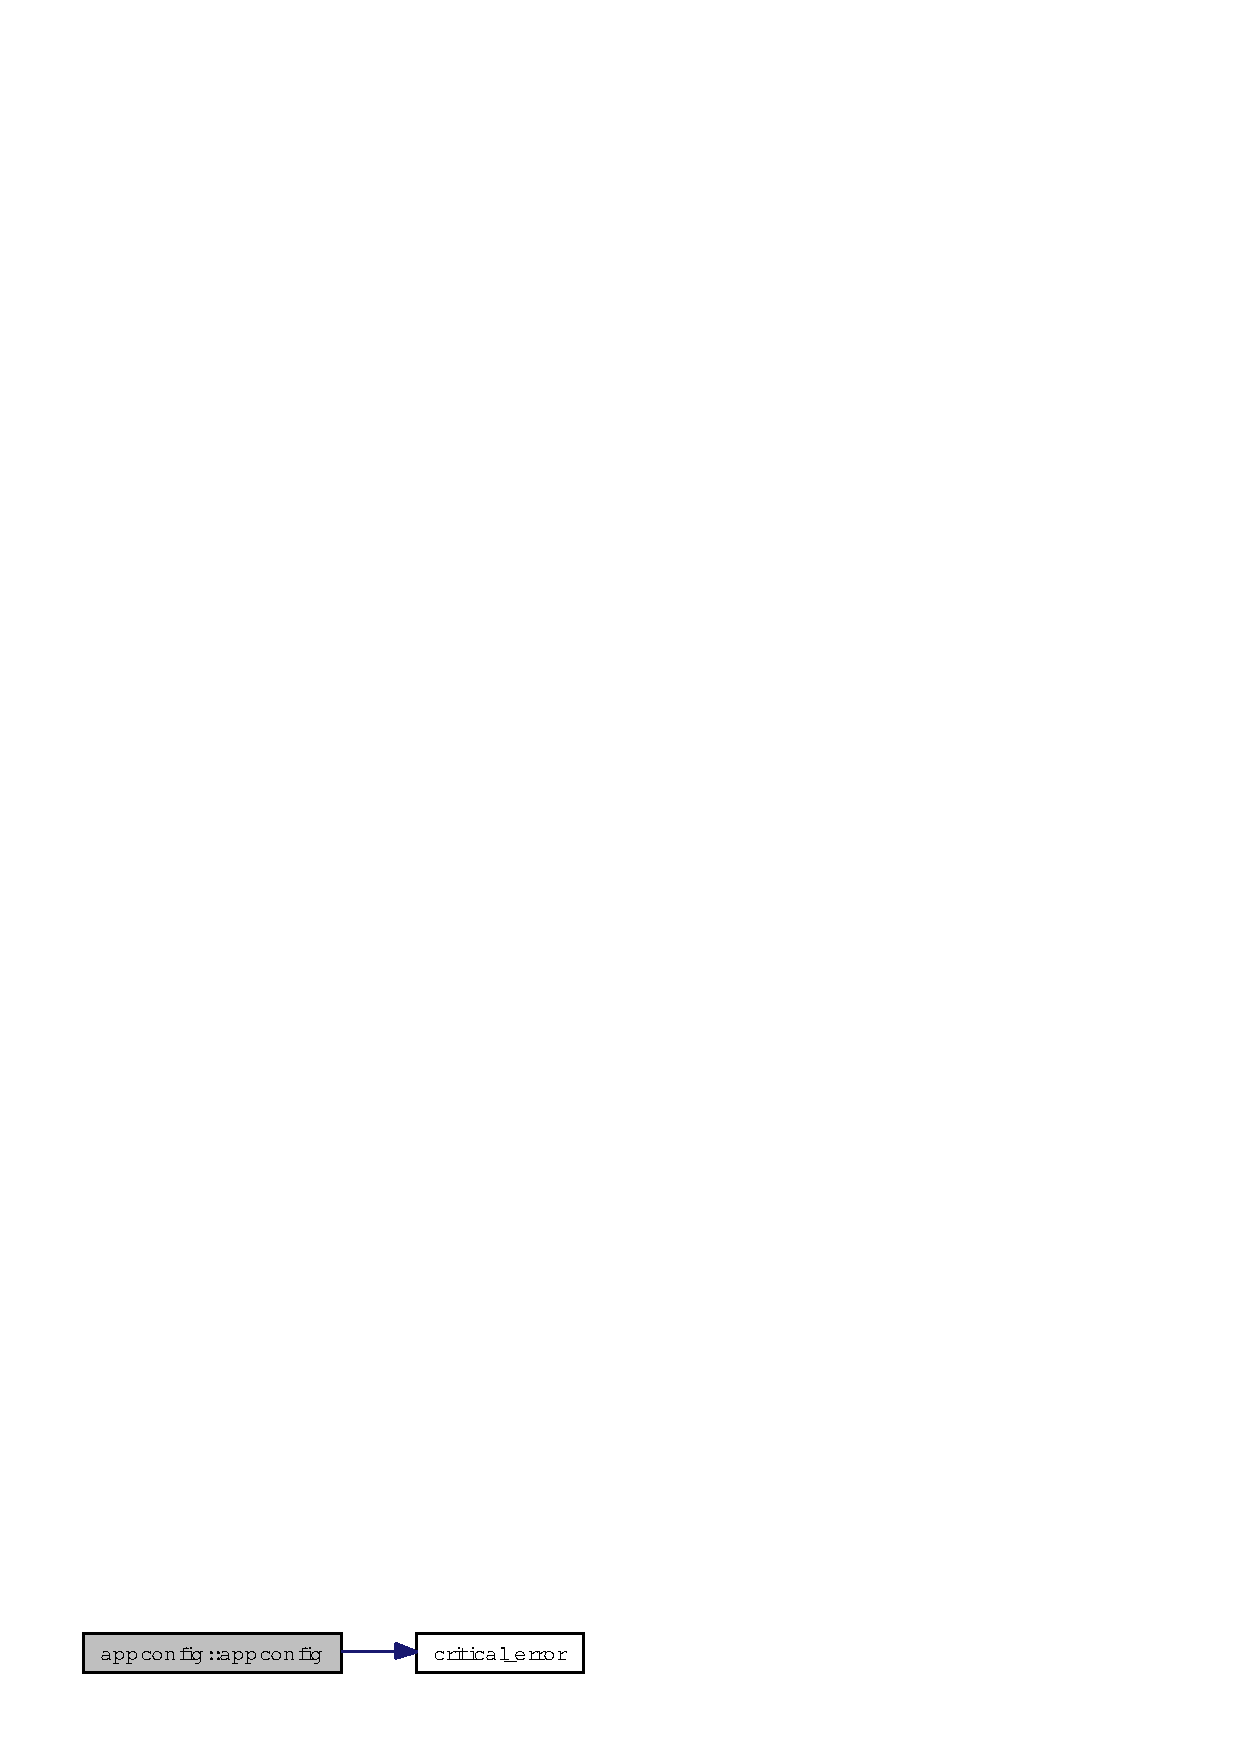
\includegraphics[width=142pt]{classappconfig_41b9c49818b354cef430735da328680e_cgraph}
\end{center}
\end{figure}
\index{appconfig@{appconfig}!~appconfig@{$\sim$appconfig}}
\index{~appconfig@{$\sim$appconfig}!appconfig@{appconfig}}
\subsubsection{\setlength{\rightskip}{0pt plus 5cm}appconfig::$\sim$appconfig ()}\label{classappconfig_df61bed4f7f8f151b8d0a839b386335f}




Definition at line 27 of file appconfig.cpp.

\subsection{Member Function Documentation}
\index{appconfig@{appconfig}!get_tetradir@{get\_\-tetradir}}
\index{get_tetradir@{get\_\-tetradir}!appconfig@{appconfig}}
\subsubsection{\setlength{\rightskip}{0pt plus 5cm}QString appconfig::get\_\-tetradir (void)}\label{classappconfig_3d61e98d919332ceb6acb2e03d8f848b}




Definition at line 62 of file appconfig.cpp.

References get\_\-parameter().

Referenced by recordtabledata::delete\_\-record(), recordtablescreen::get\_\-fullfilename\_\-of\_\-currentitem(), recordtabledata::get\_\-text(), treescreen::init\_\-knowtree(), recordtabledata::insert\_\-new\_\-record(), treescreen::save\_\-knowtree(), and recordtablescreen::select().

Here is the call graph for this function:\begin{figure}[H]
\begin{center}
\leavevmode
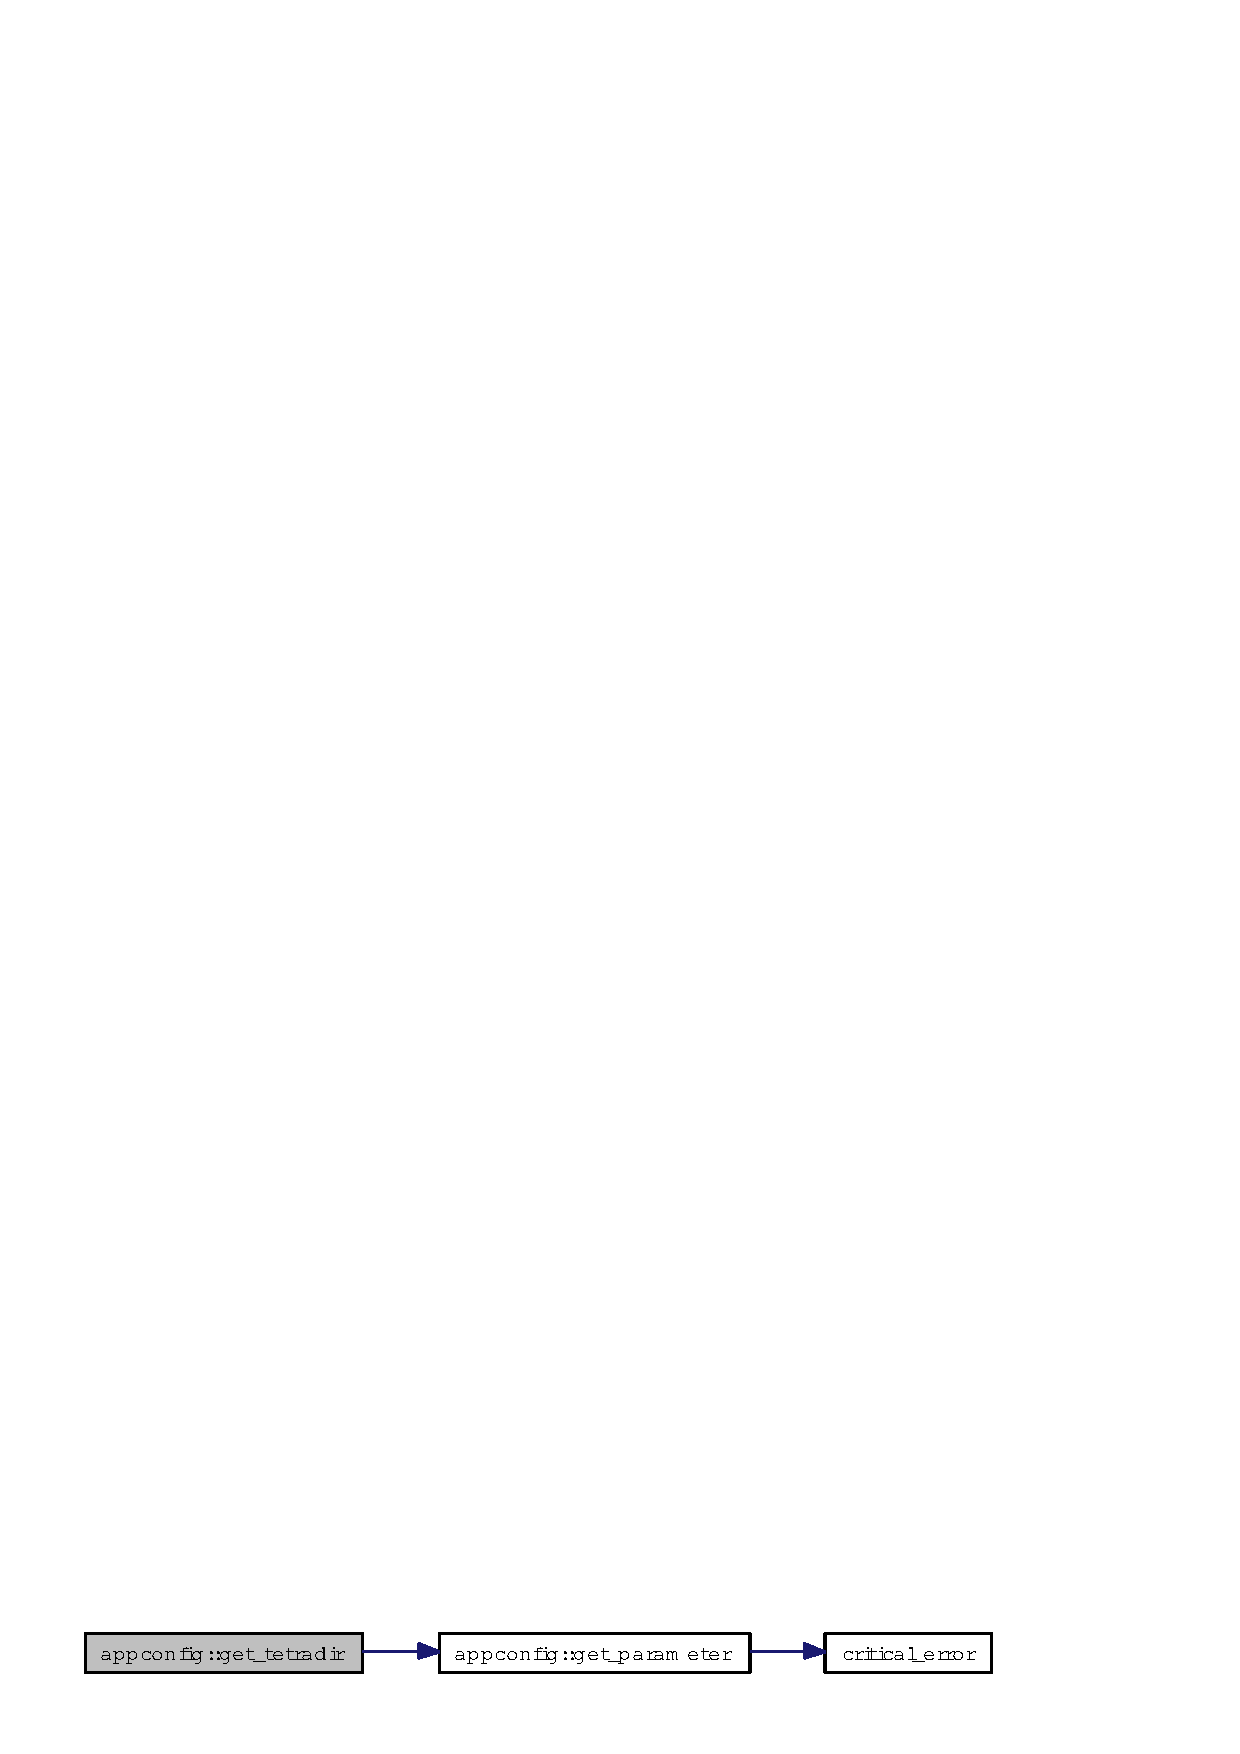
\includegraphics[width=240pt]{classappconfig_3d61e98d919332ceb6acb2e03d8f848b_cgraph}
\end{center}
\end{figure}


Here is the caller graph for this function:\begin{figure}[H]
\begin{center}
\leavevmode
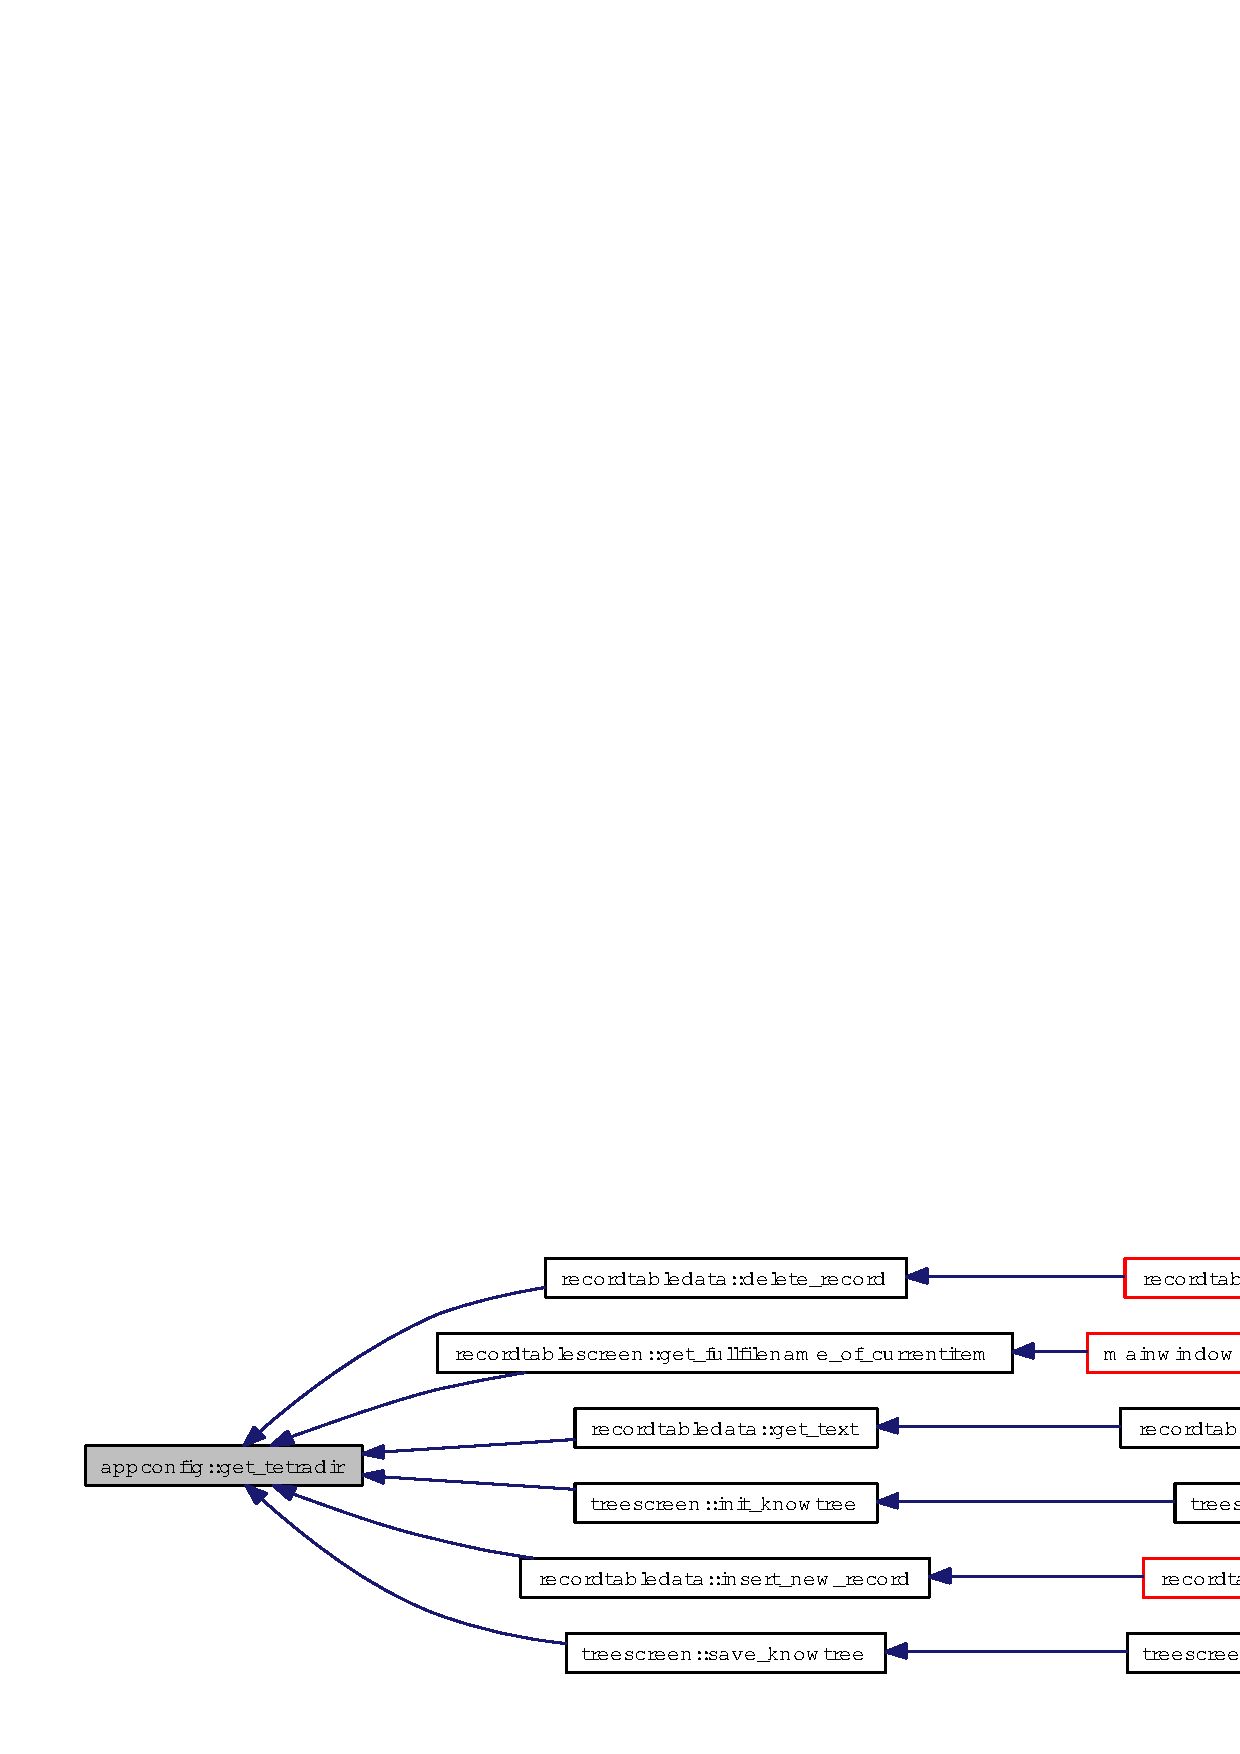
\includegraphics[width=370pt]{classappconfig_3d61e98d919332ceb6acb2e03d8f848b_icgraph}
\end{center}
\end{figure}
\index{appconfig@{appconfig}!set_tetradir@{set\_\-tetradir}}
\index{set_tetradir@{set\_\-tetradir}!appconfig@{appconfig}}
\subsubsection{\setlength{\rightskip}{0pt plus 5cm}bool appconfig::set\_\-tetradir (QString {\em dirname})}\label{classappconfig_f90278aac0141bdc3d1f2869e0b85733}




Definition at line 47 of file appconfig.cpp.

References conf.\index{appconfig@{appconfig}!get_trashdir@{get\_\-trashdir}}
\index{get_trashdir@{get\_\-trashdir}!appconfig@{appconfig}}
\subsubsection{\setlength{\rightskip}{0pt plus 5cm}QString appconfig::get\_\-trashdir (void)}\label{classappconfig_aa1dba748c982e0759e1c13490a68ccf}




Definition at line 84 of file appconfig.cpp.

References get\_\-parameter().

Referenced by remove\_\-dir(), mainwindow::save\_\-current\_\-record\_\-text(), and treescreen::save\_\-knowtree().

Here is the call graph for this function:\begin{figure}[H]
\begin{center}
\leavevmode
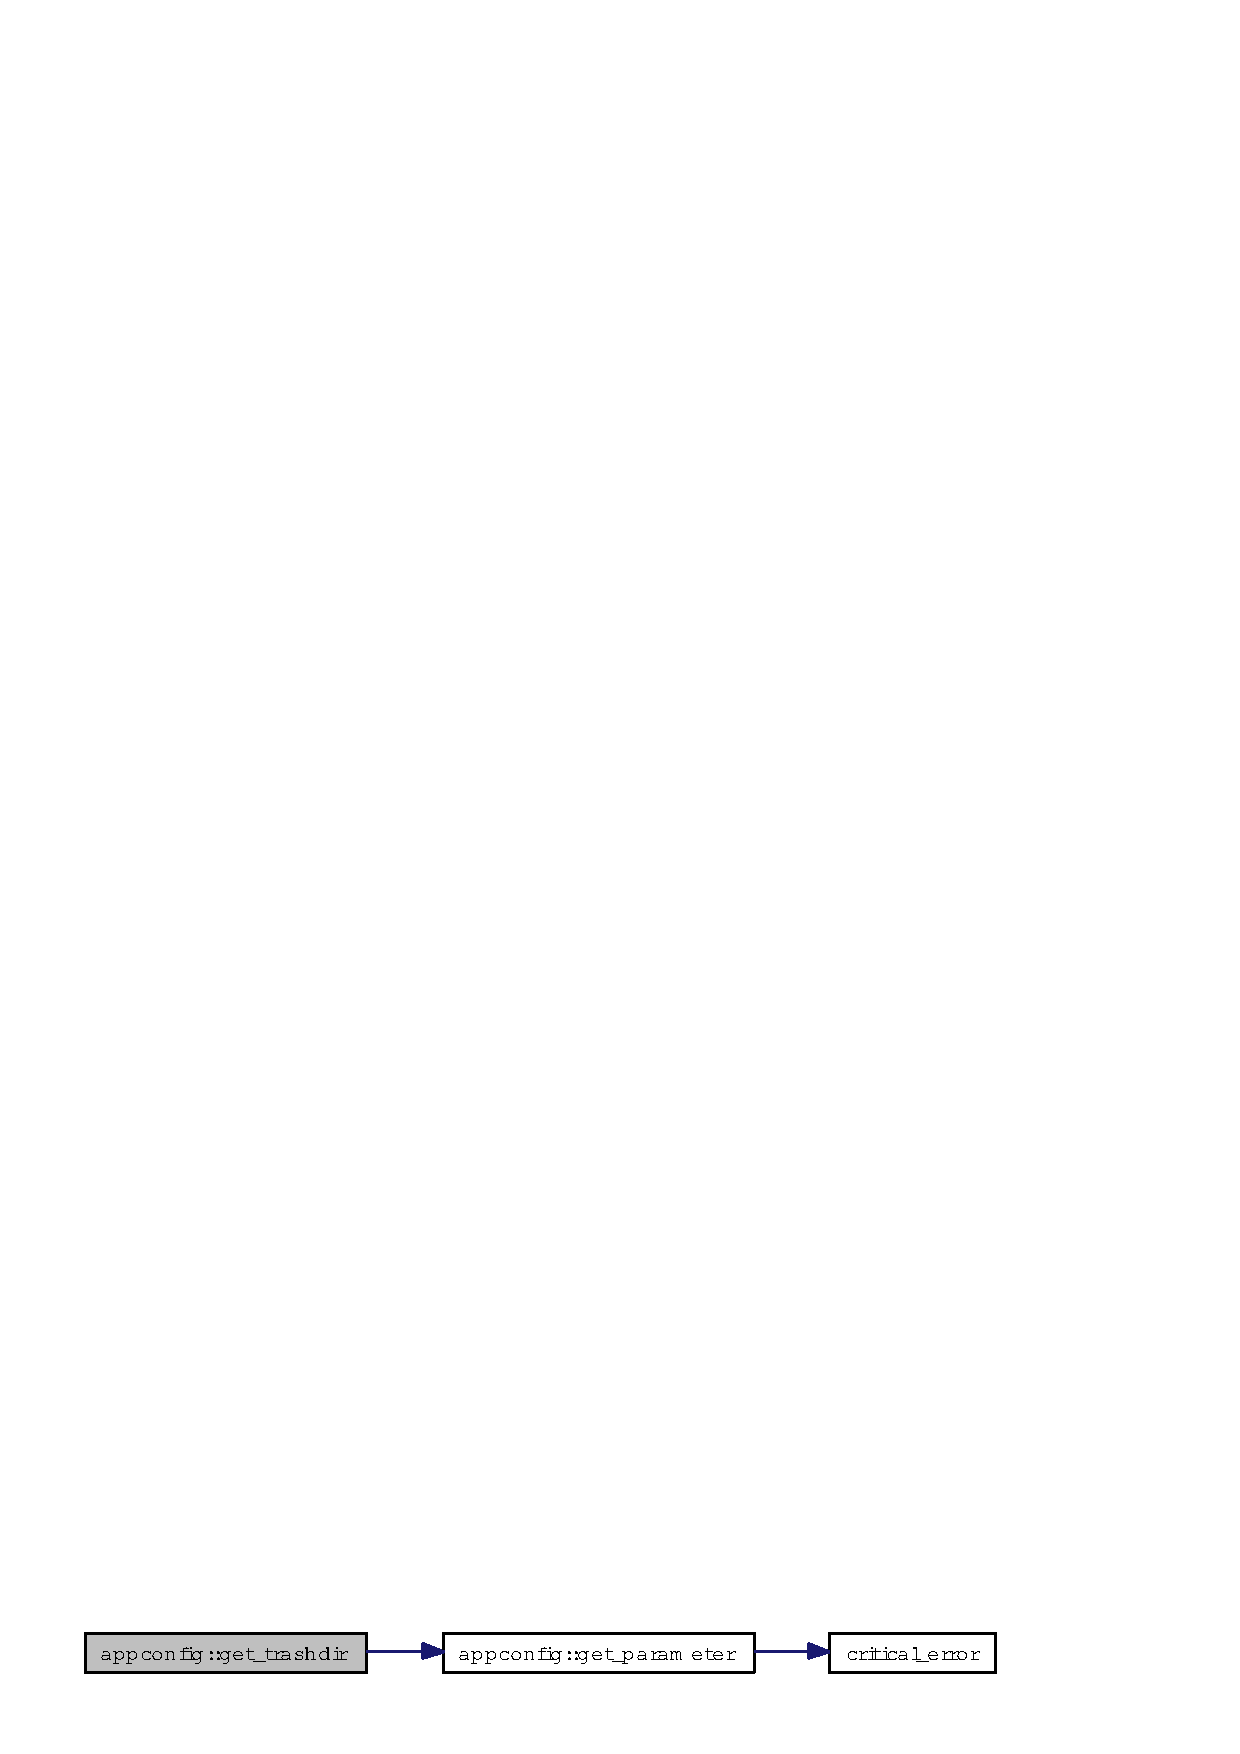
\includegraphics[width=241pt]{classappconfig_aa1dba748c982e0759e1c13490a68ccf_cgraph}
\end{center}
\end{figure}


Here is the caller graph for this function:\begin{figure}[H]
\begin{center}
\leavevmode
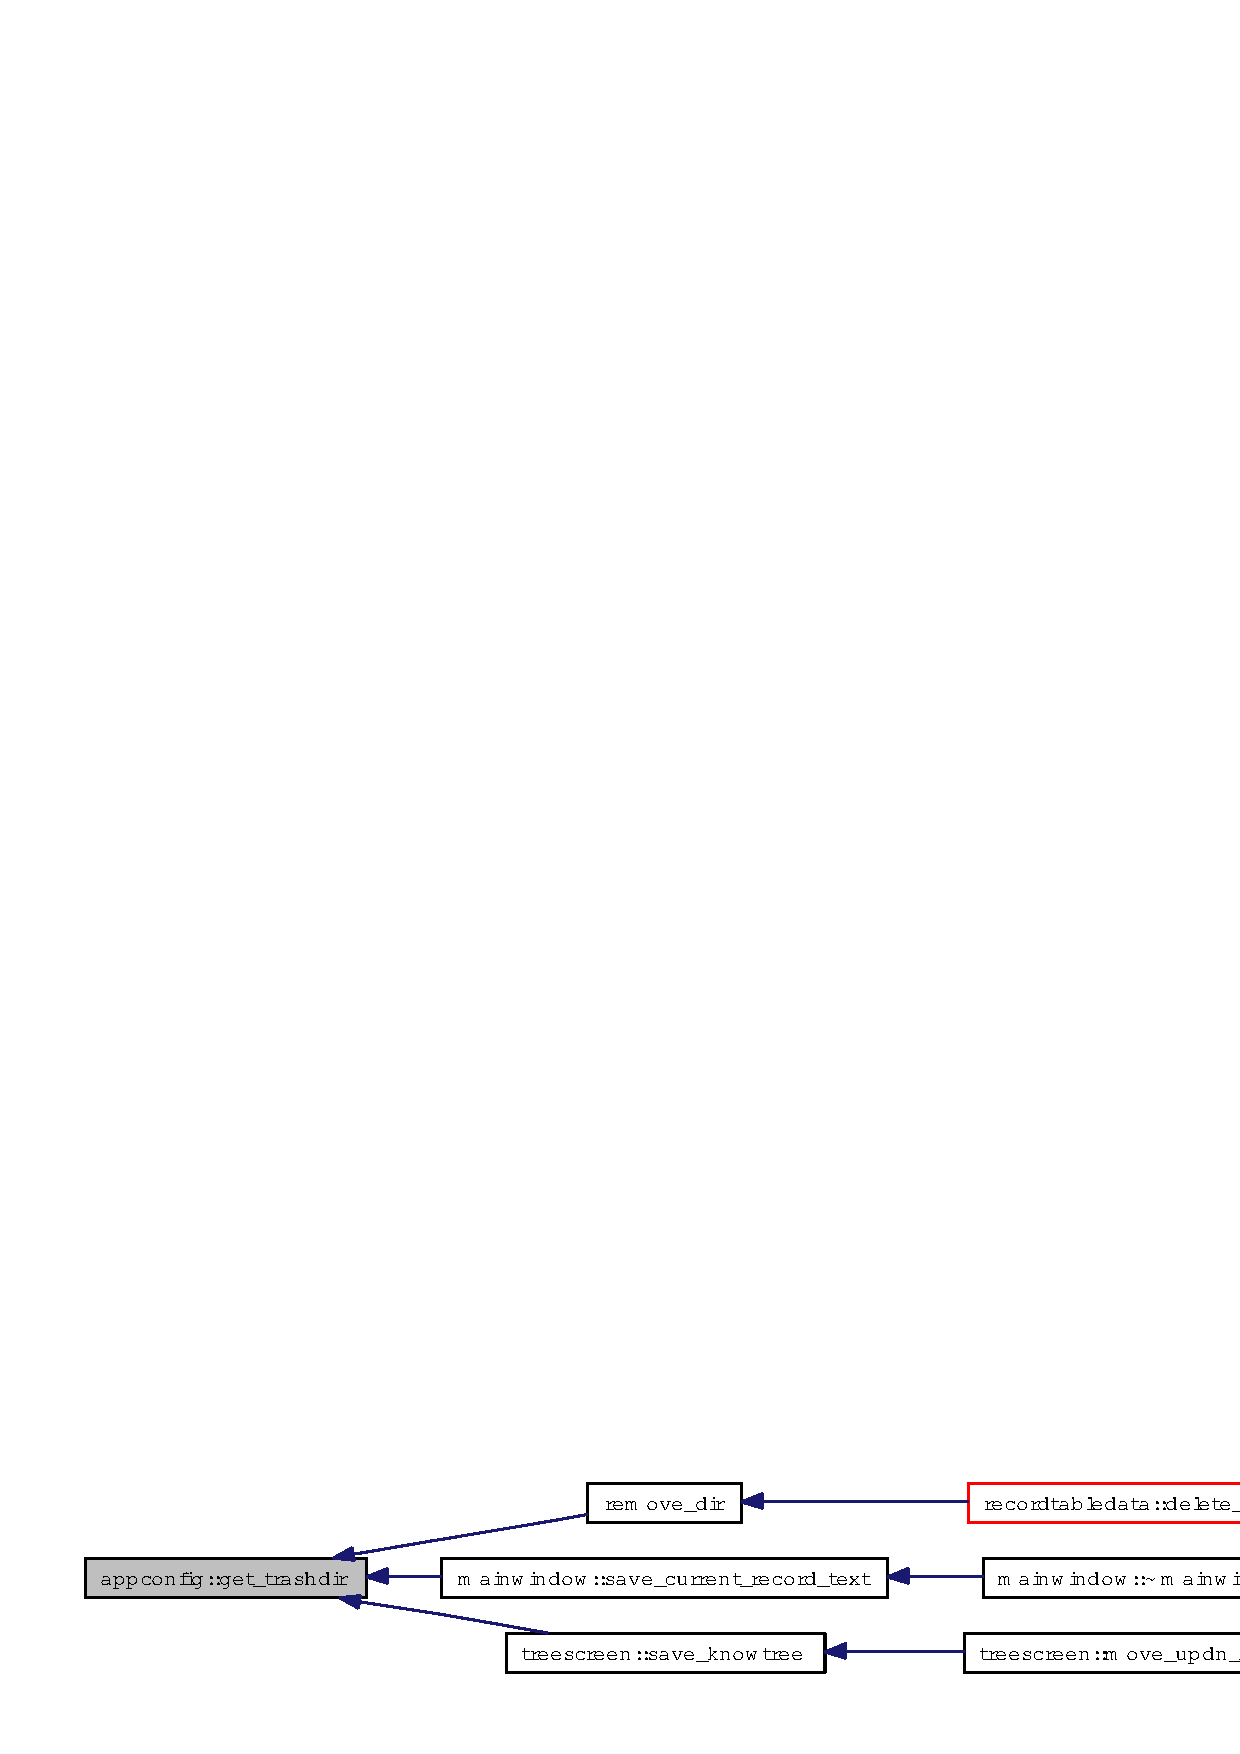
\includegraphics[width=322pt]{classappconfig_aa1dba748c982e0759e1c13490a68ccf_icgraph}
\end{center}
\end{figure}
\index{appconfig@{appconfig}!set_trashdir@{set\_\-trashdir}}
\index{set_trashdir@{set\_\-trashdir}!appconfig@{appconfig}}
\subsubsection{\setlength{\rightskip}{0pt plus 5cm}bool appconfig::set\_\-trashdir (QString {\em dirname})}\label{classappconfig_05797f15022b1c454842471047bc3bf8}




Definition at line 69 of file appconfig.cpp.

References conf.\index{appconfig@{appconfig}!get_lastnotenum@{get\_\-lastnotenum}}
\index{get_lastnotenum@{get\_\-lastnotenum}!appconfig@{appconfig}}
\subsubsection{\setlength{\rightskip}{0pt plus 5cm}int appconfig::get\_\-lastnotenum (void)}\label{classappconfig_0291790bcb173b674f70950181f70545}




Definition at line 91 of file appconfig.cpp.

References get\_\-parameter().

Referenced by inc\_\-lastnotenum().

Here is the call graph for this function:\begin{figure}[H]
\begin{center}
\leavevmode
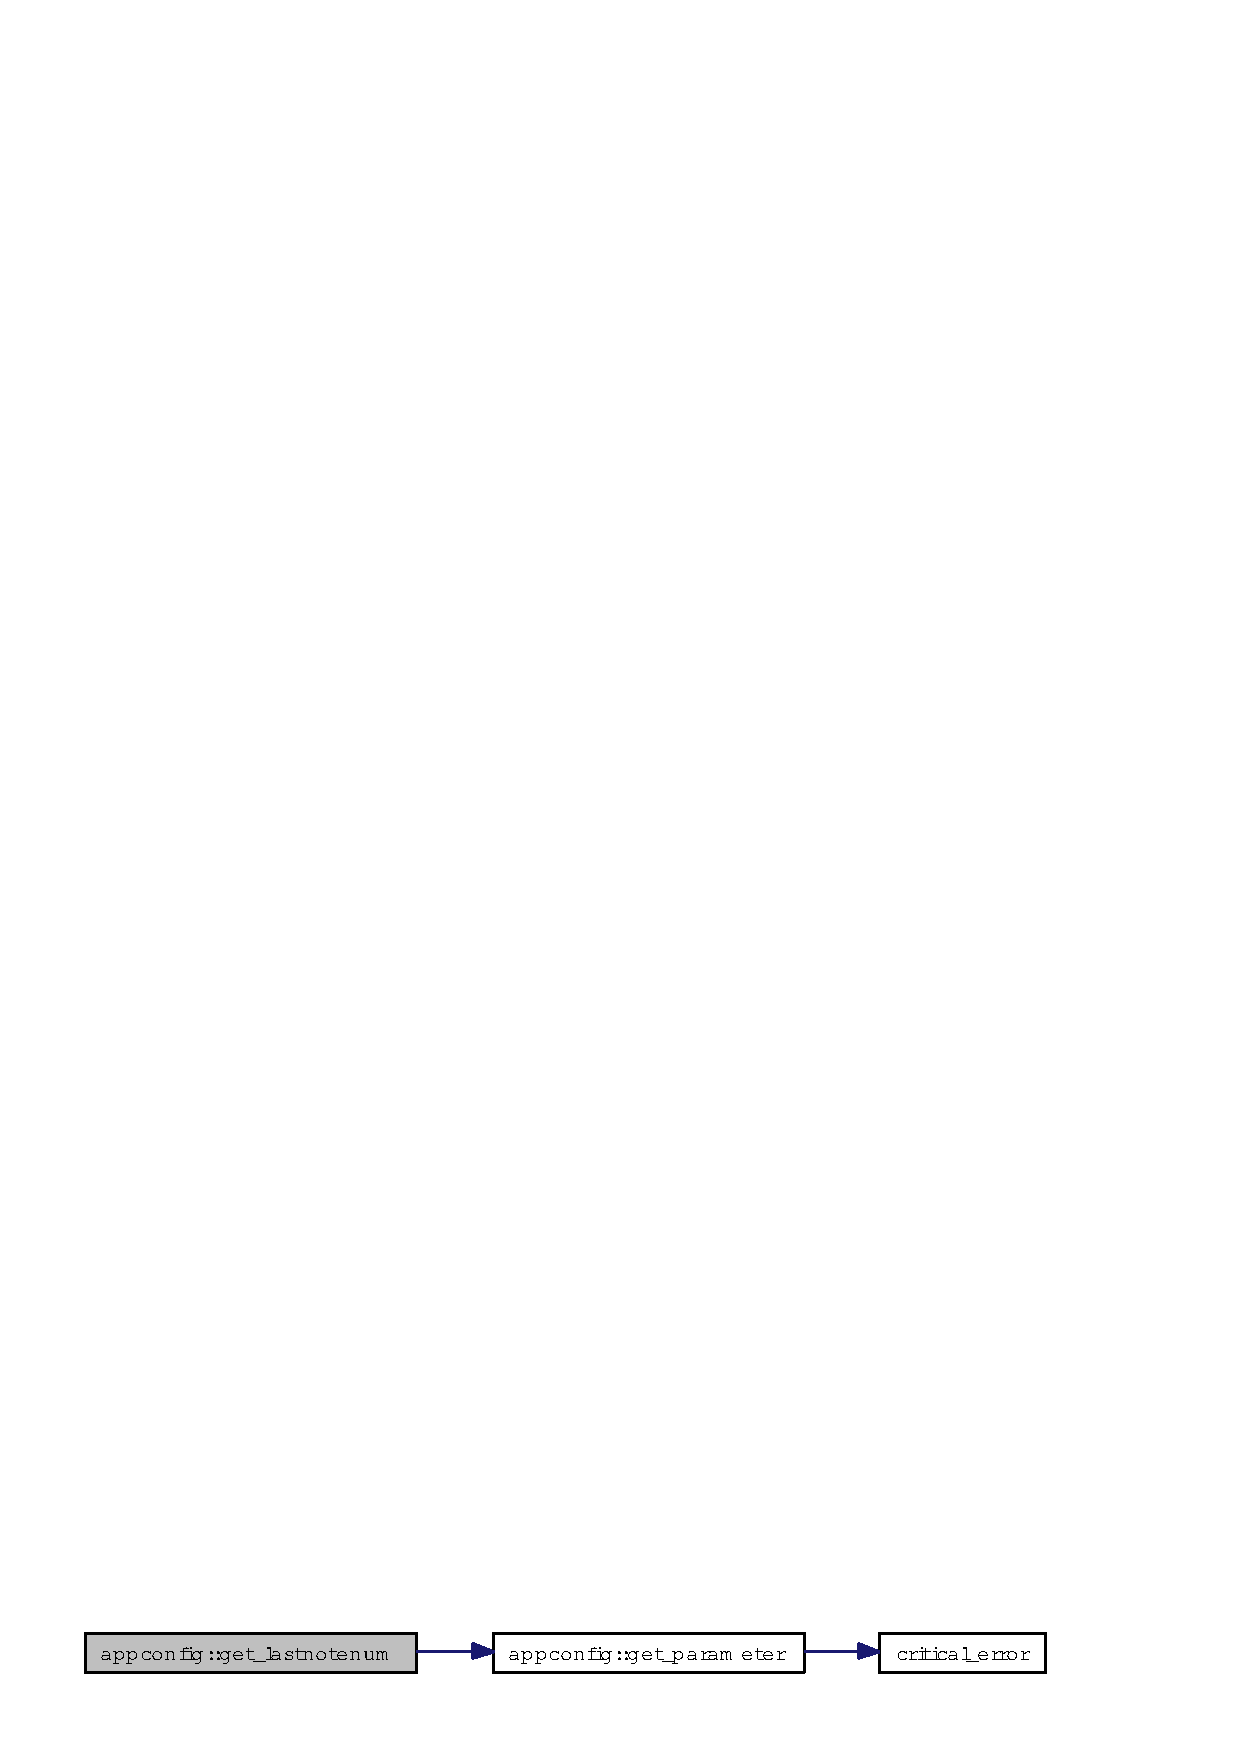
\includegraphics[width=253pt]{classappconfig_0291790bcb173b674f70950181f70545_cgraph}
\end{center}
\end{figure}


Here is the caller graph for this function:\begin{figure}[H]
\begin{center}
\leavevmode
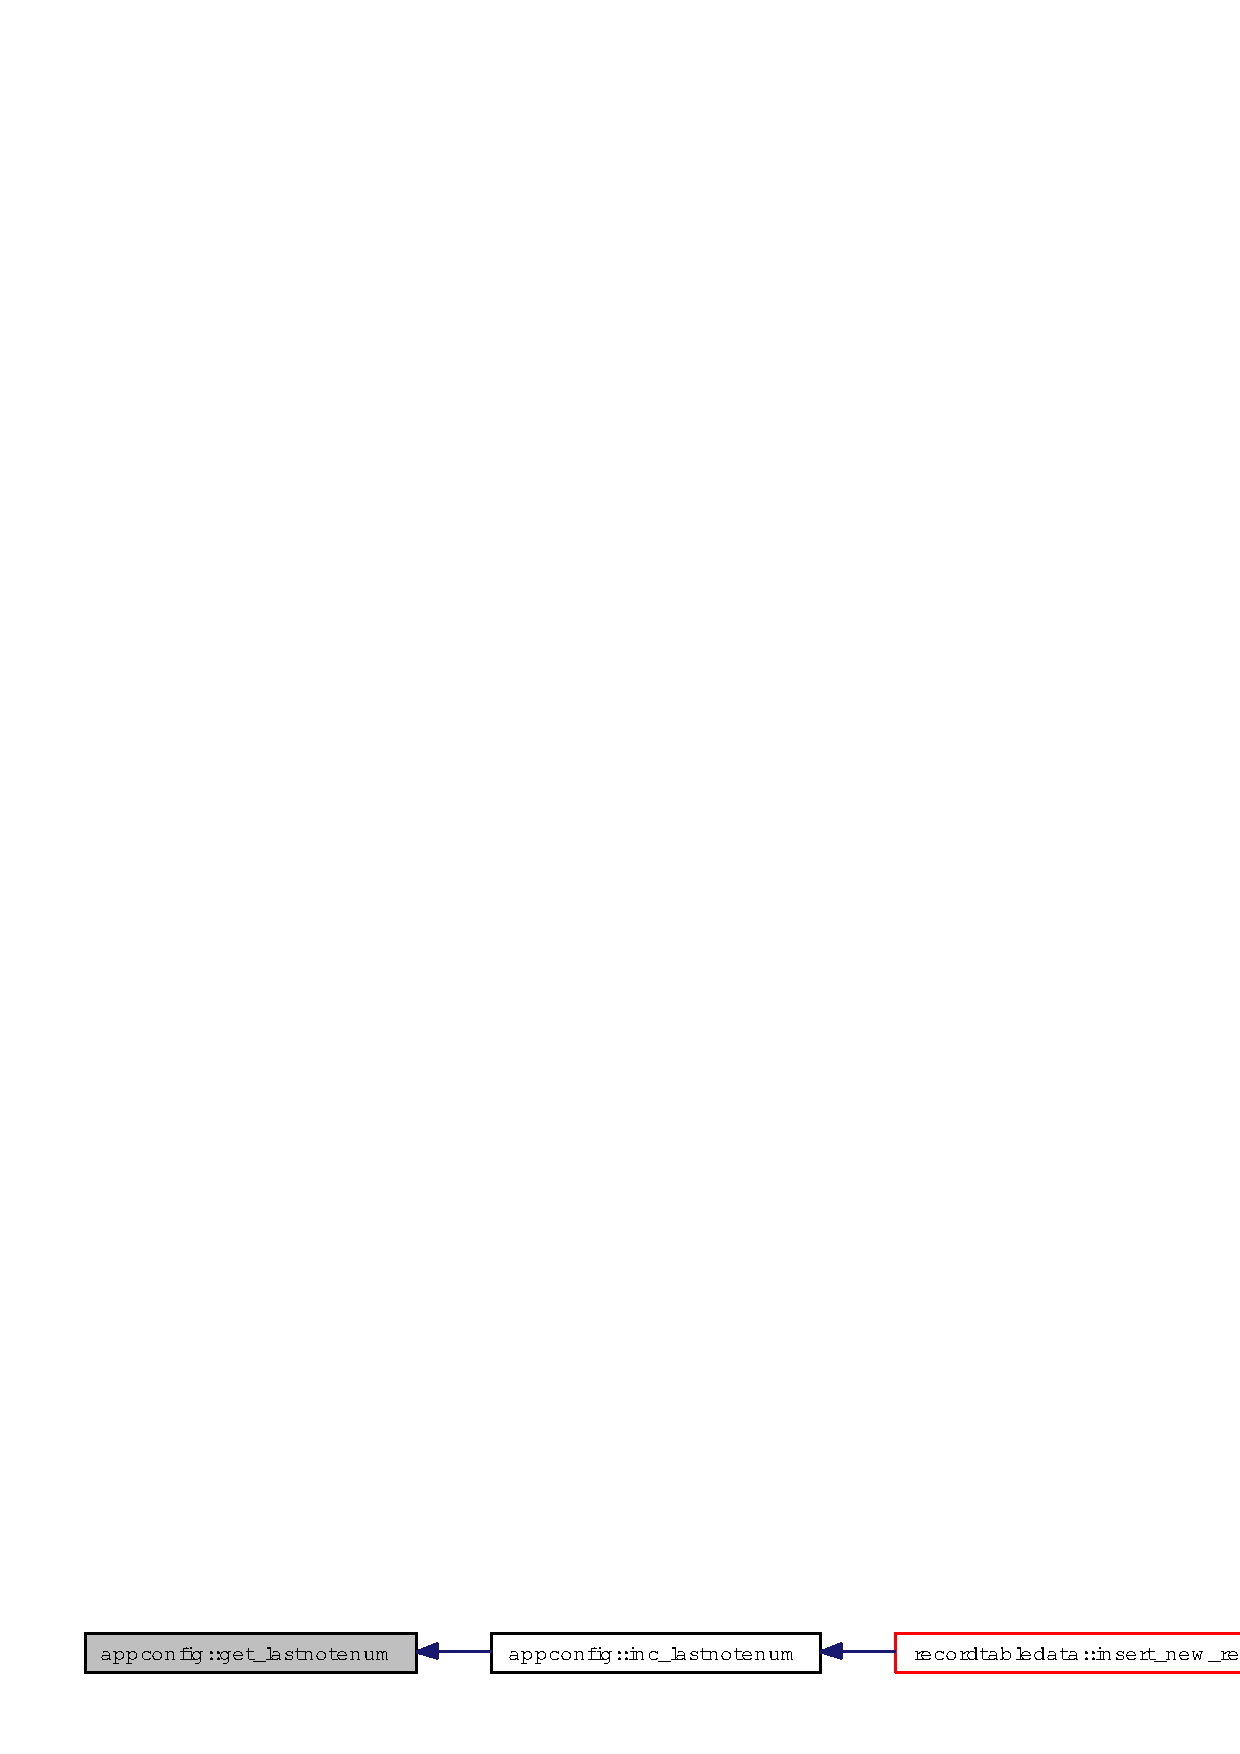
\includegraphics[width=315pt]{classappconfig_0291790bcb173b674f70950181f70545_icgraph}
\end{center}
\end{figure}
\index{appconfig@{appconfig}!get_lastnotenum_as_line@{get\_\-lastnotenum\_\-as\_\-line}}
\index{get_lastnotenum_as_line@{get\_\-lastnotenum\_\-as\_\-line}!appconfig@{appconfig}}
\subsubsection{\setlength{\rightskip}{0pt plus 5cm}QString appconfig::get\_\-lastnotenum\_\-as\_\-line (void)}\label{classappconfig_2a324f08a97ea456e79d59fe16877000}




Definition at line 103 of file appconfig.cpp.

References get\_\-parameter().

Referenced by recordtabledata::insert\_\-new\_\-record().

Here is the call graph for this function:\begin{figure}[H]
\begin{center}
\leavevmode
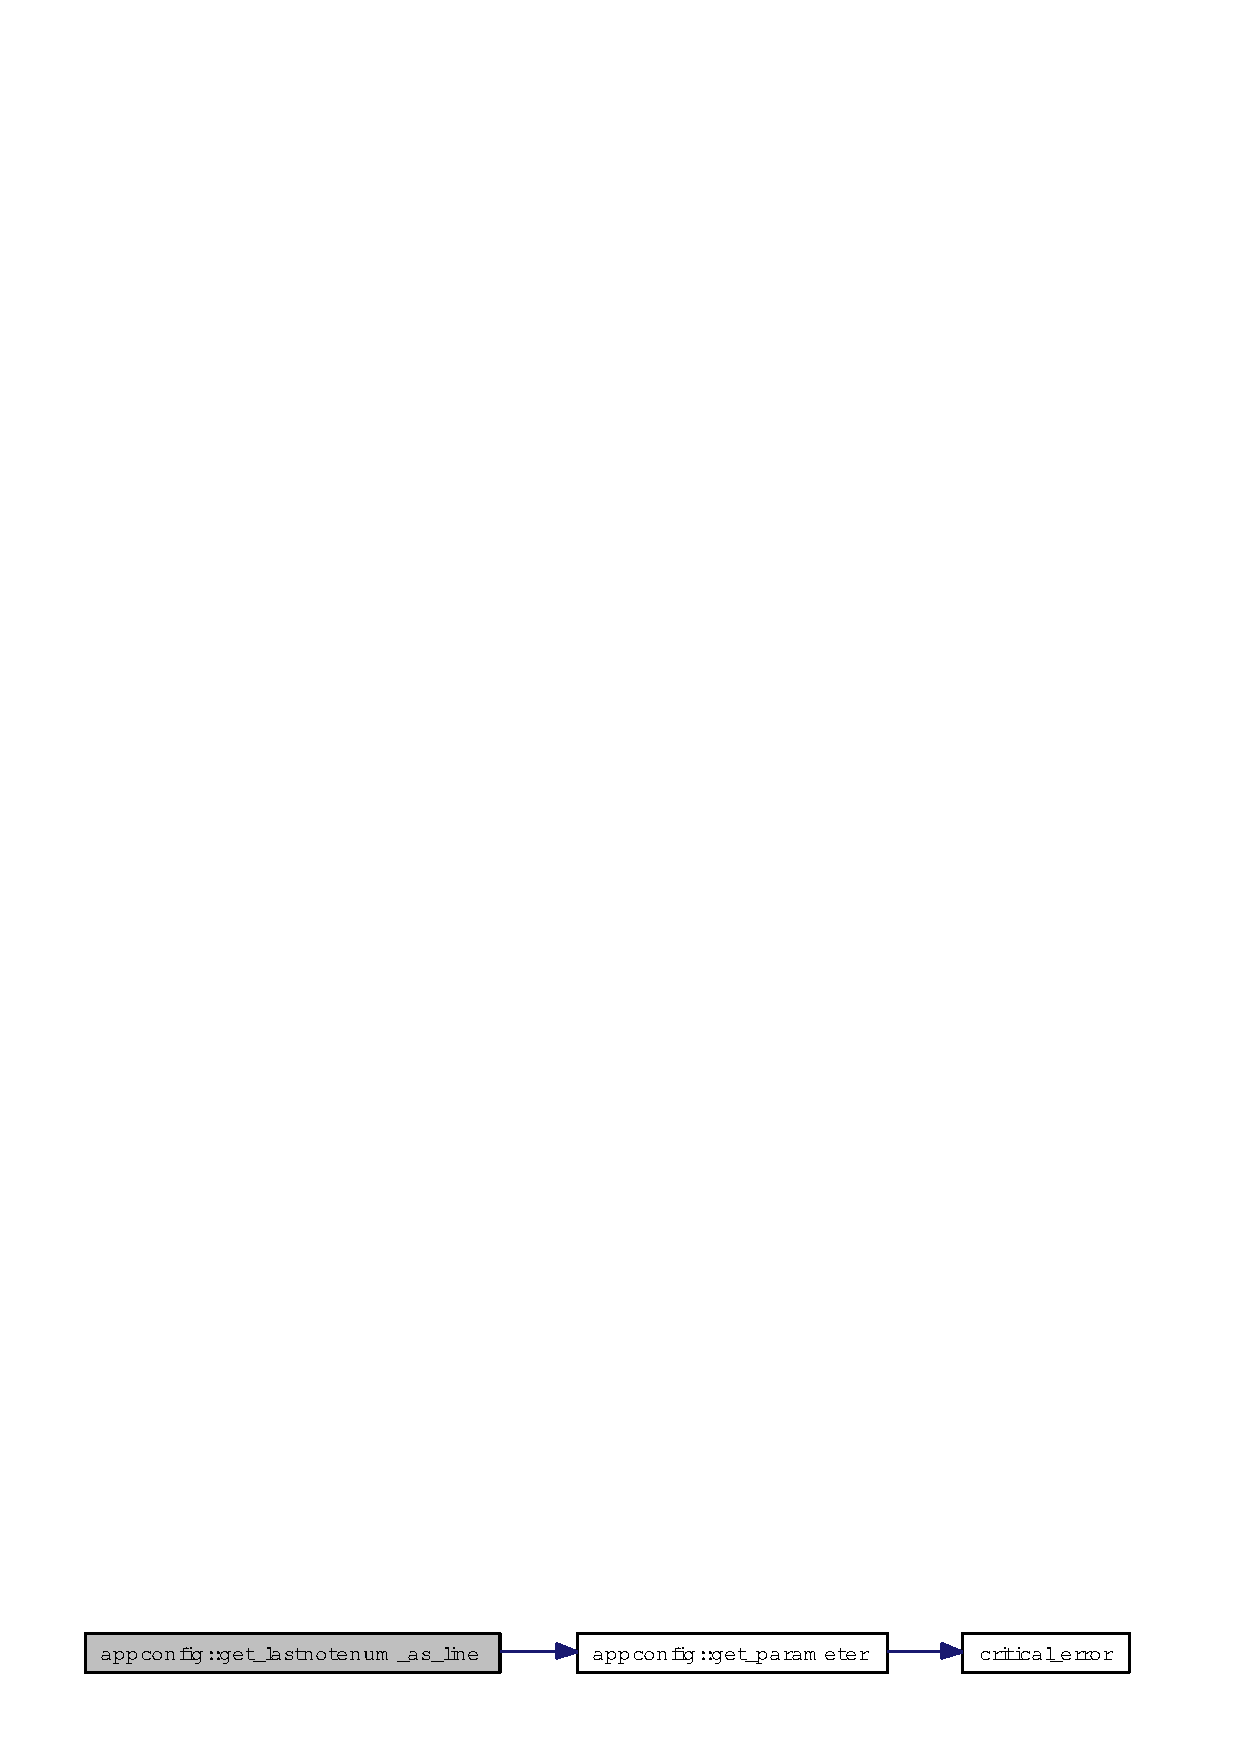
\includegraphics[width=273pt]{classappconfig_2a324f08a97ea456e79d59fe16877000_cgraph}
\end{center}
\end{figure}


Here is the caller graph for this function:\begin{figure}[H]
\begin{center}
\leavevmode
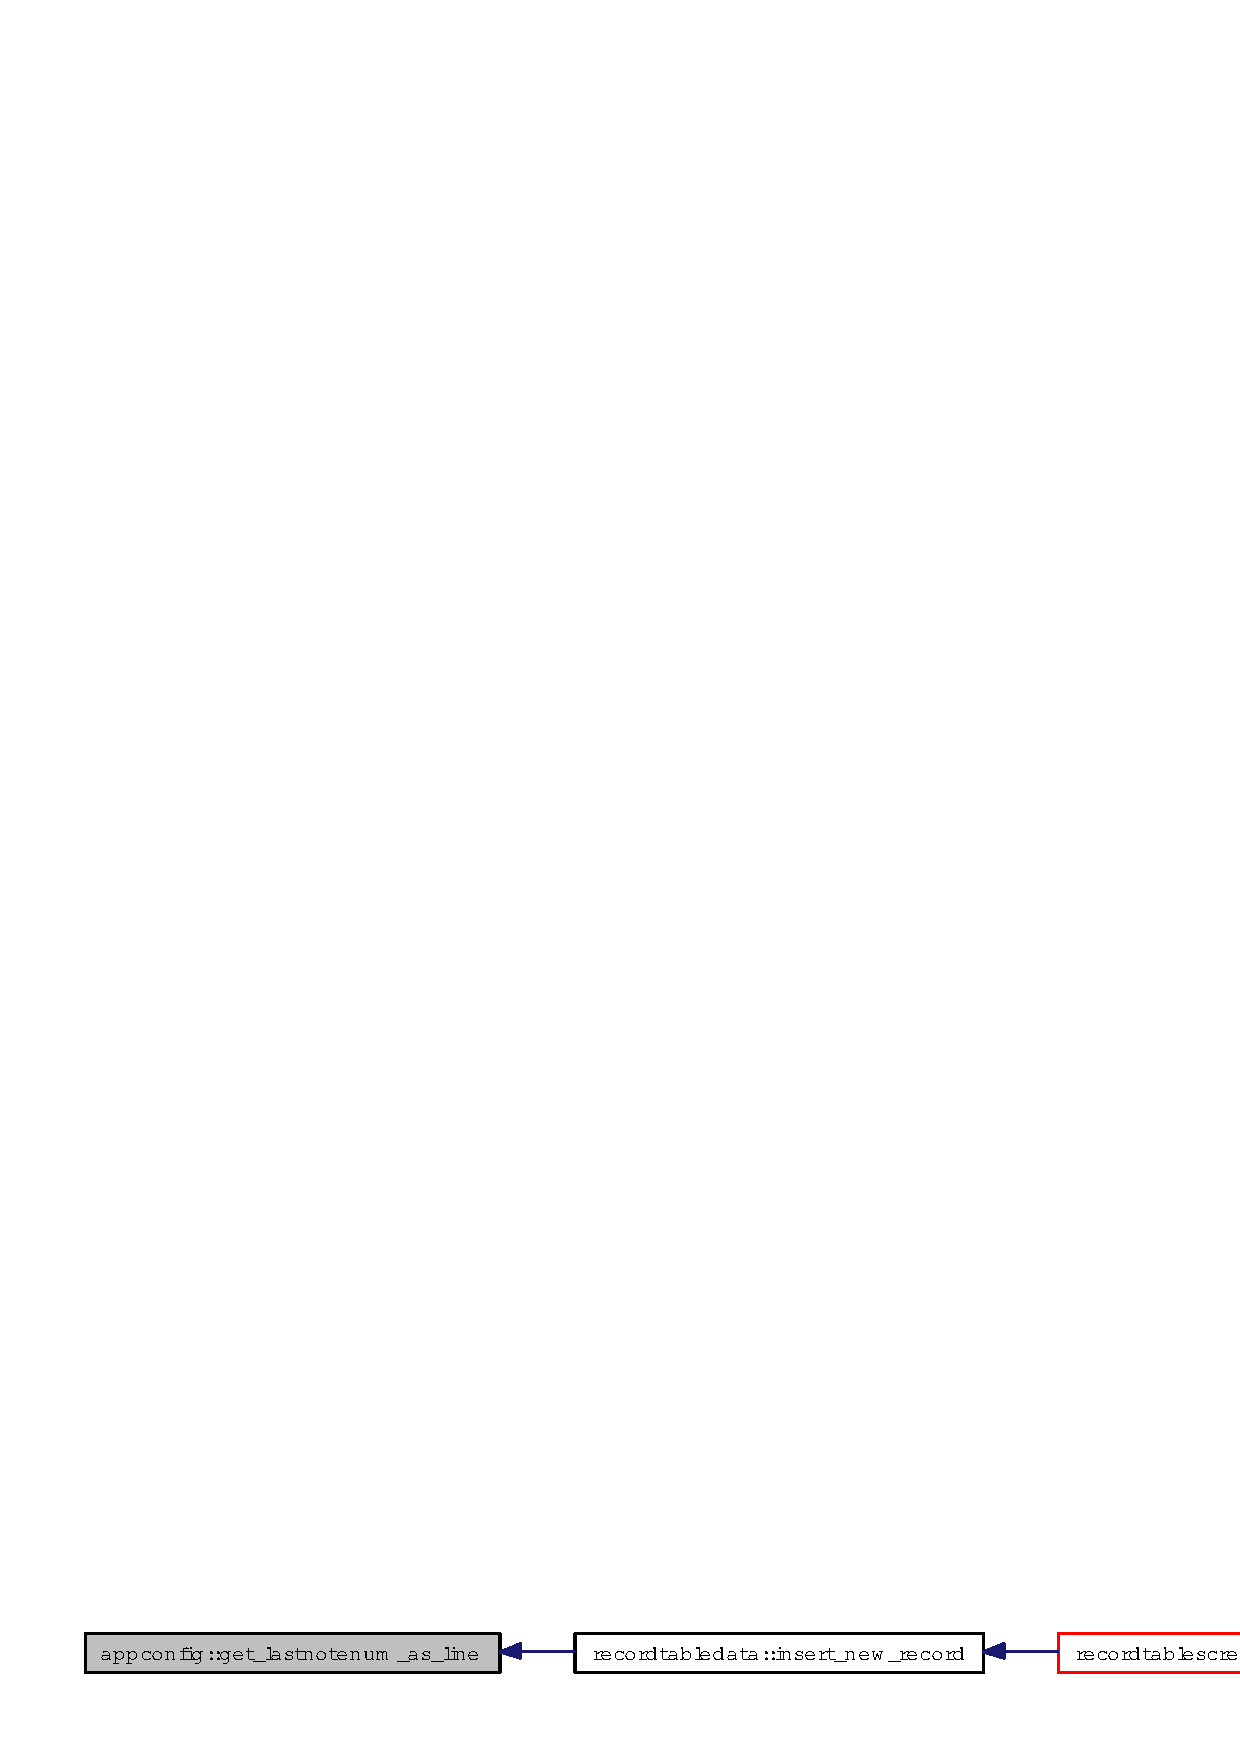
\includegraphics[width=336pt]{classappconfig_2a324f08a97ea456e79d59fe16877000_icgraph}
\end{center}
\end{figure}
\index{appconfig@{appconfig}!inc_lastnotenum@{inc\_\-lastnotenum}}
\index{inc_lastnotenum@{inc\_\-lastnotenum}!appconfig@{appconfig}}
\subsubsection{\setlength{\rightskip}{0pt plus 5cm}void appconfig::inc\_\-lastnotenum (void)}\label{classappconfig_1ac40c253c15b60755a4d50b7541abf1}




Definition at line 114 of file appconfig.cpp.

References conf, and get\_\-lastnotenum().

Referenced by recordtabledata::insert\_\-new\_\-record().

Here is the call graph for this function:\begin{figure}[H]
\begin{center}
\leavevmode
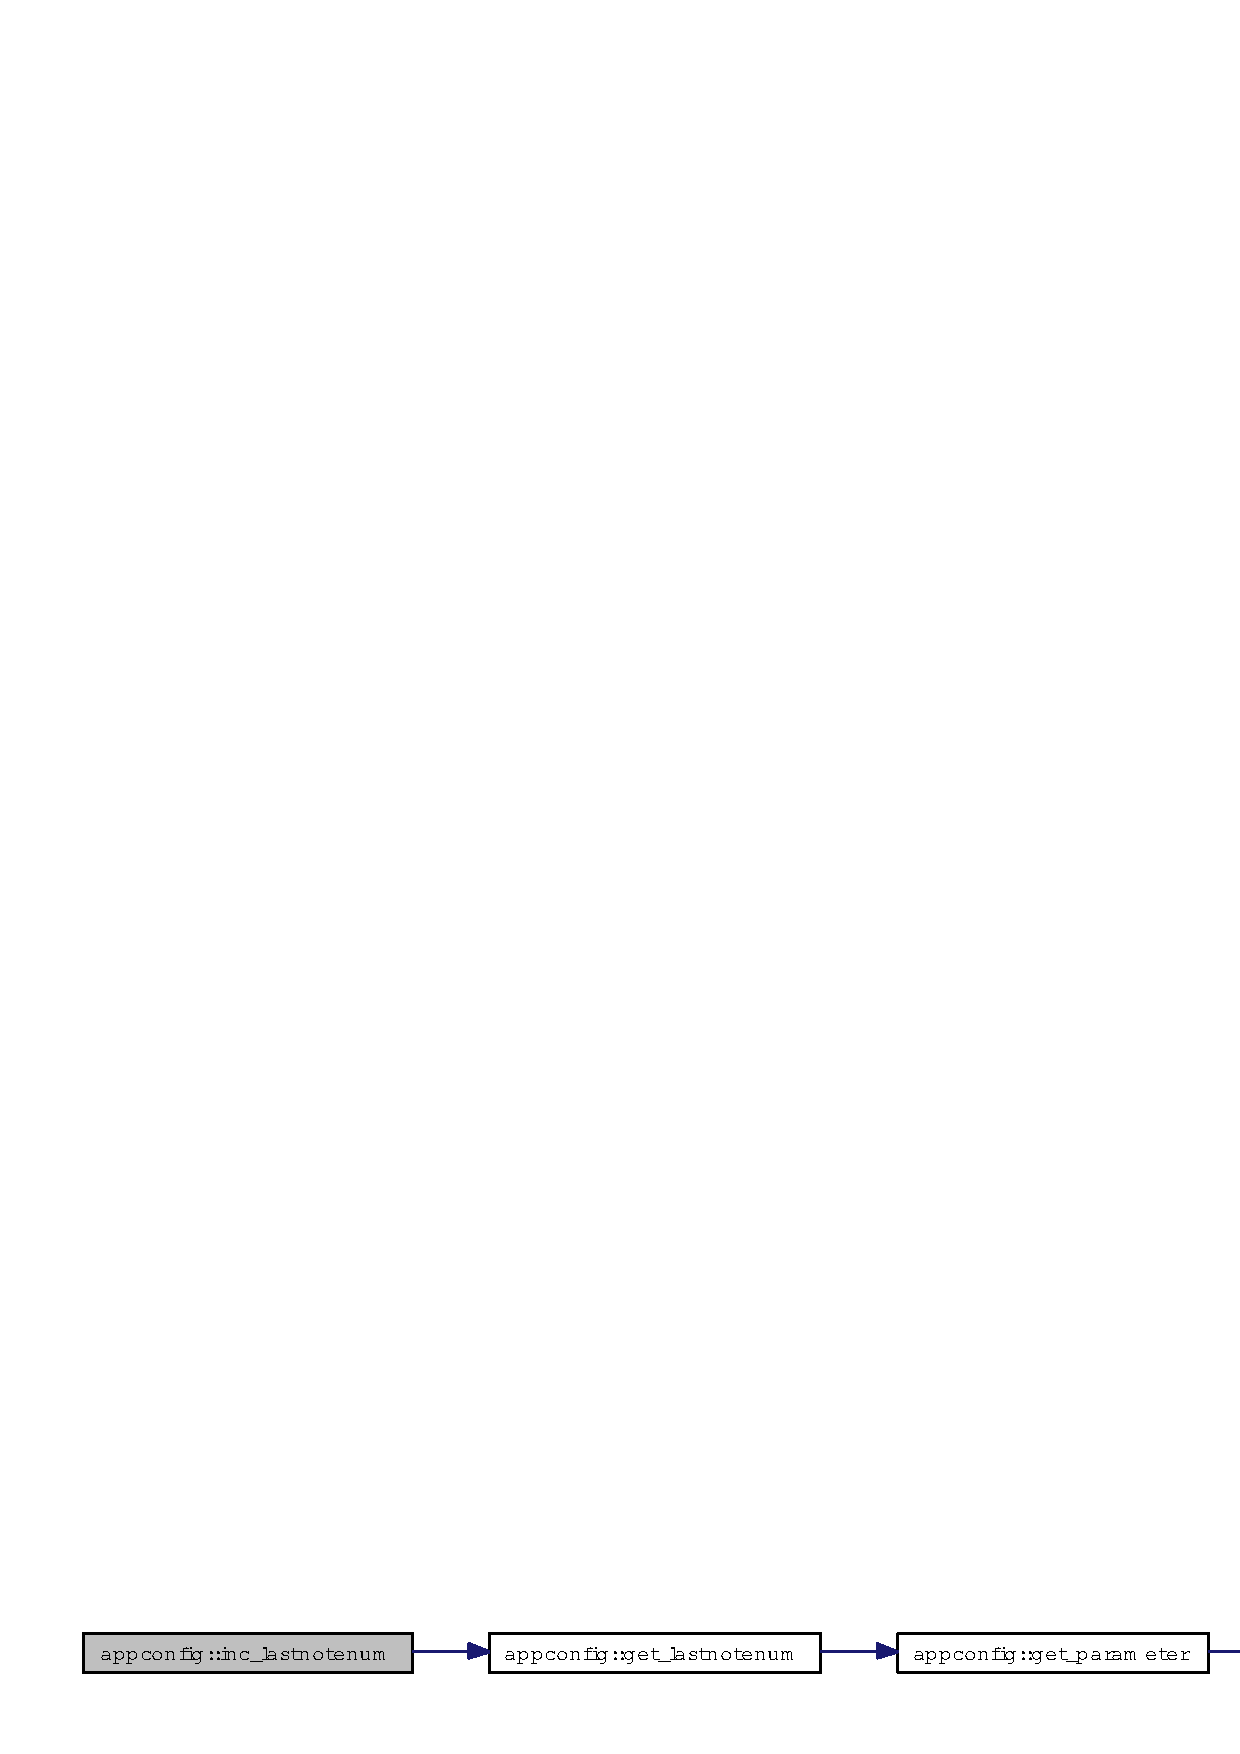
\includegraphics[width=350pt]{classappconfig_1ac40c253c15b60755a4d50b7541abf1_cgraph}
\end{center}
\end{figure}


Here is the caller graph for this function:\begin{figure}[H]
\begin{center}
\leavevmode
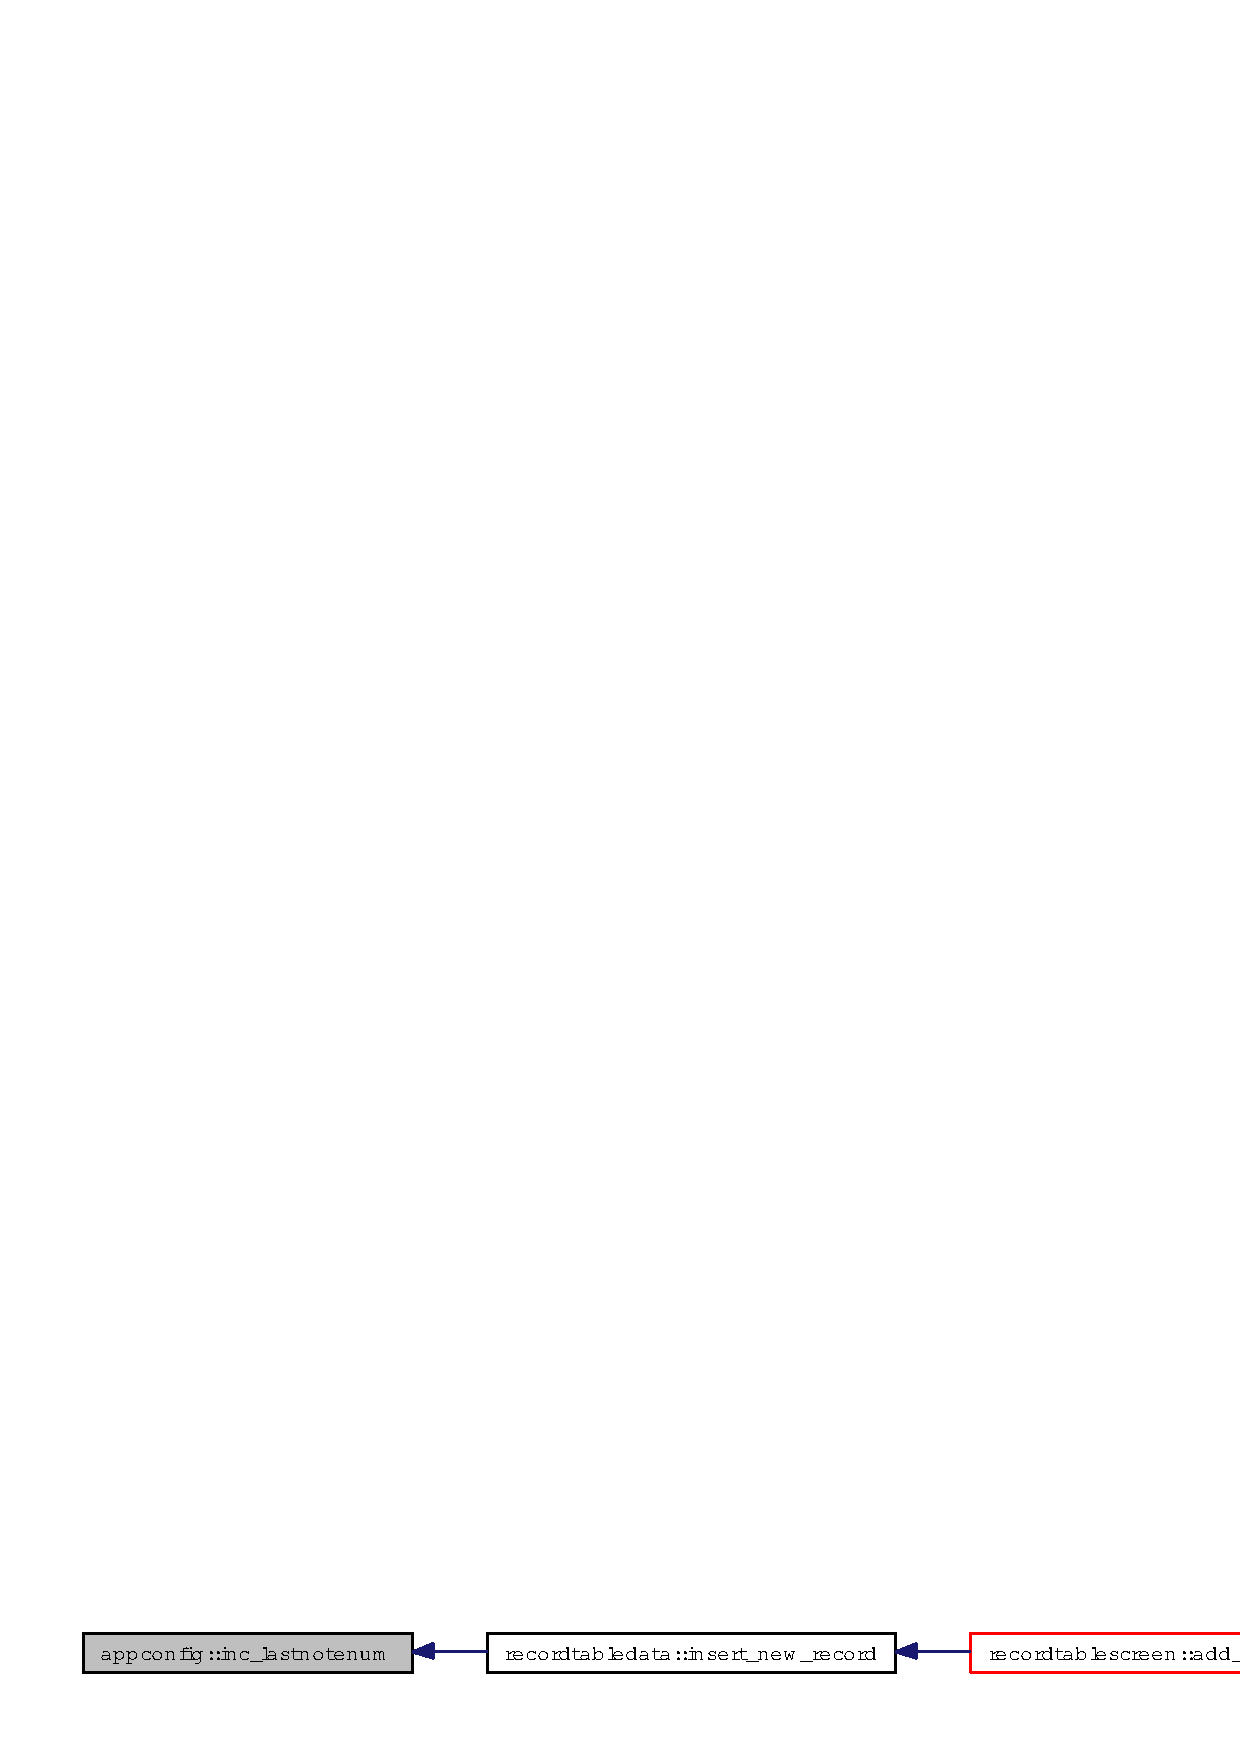
\includegraphics[width=315pt]{classappconfig_1ac40c253c15b60755a4d50b7541abf1_icgraph}
\end{center}
\end{figure}
\index{appconfig@{appconfig}!get_lastidnum@{get\_\-lastidnum}}
\index{get_lastidnum@{get\_\-lastidnum}!appconfig@{appconfig}}
\subsubsection{\setlength{\rightskip}{0pt plus 5cm}int appconfig::get\_\-lastidnum (void)}\label{classappconfig_098e273bf84b2ce0ffcf69ce98d99acb}




Definition at line 126 of file appconfig.cpp.

References get\_\-parameter().

Referenced by inc\_\-lastidnum(), treescreen::ins\_\-branch(), treescreen::ins\_\-subbranch(), and recordtabledata::insert\_\-new\_\-record().

Here is the call graph for this function:\begin{figure}[H]
\begin{center}
\leavevmode
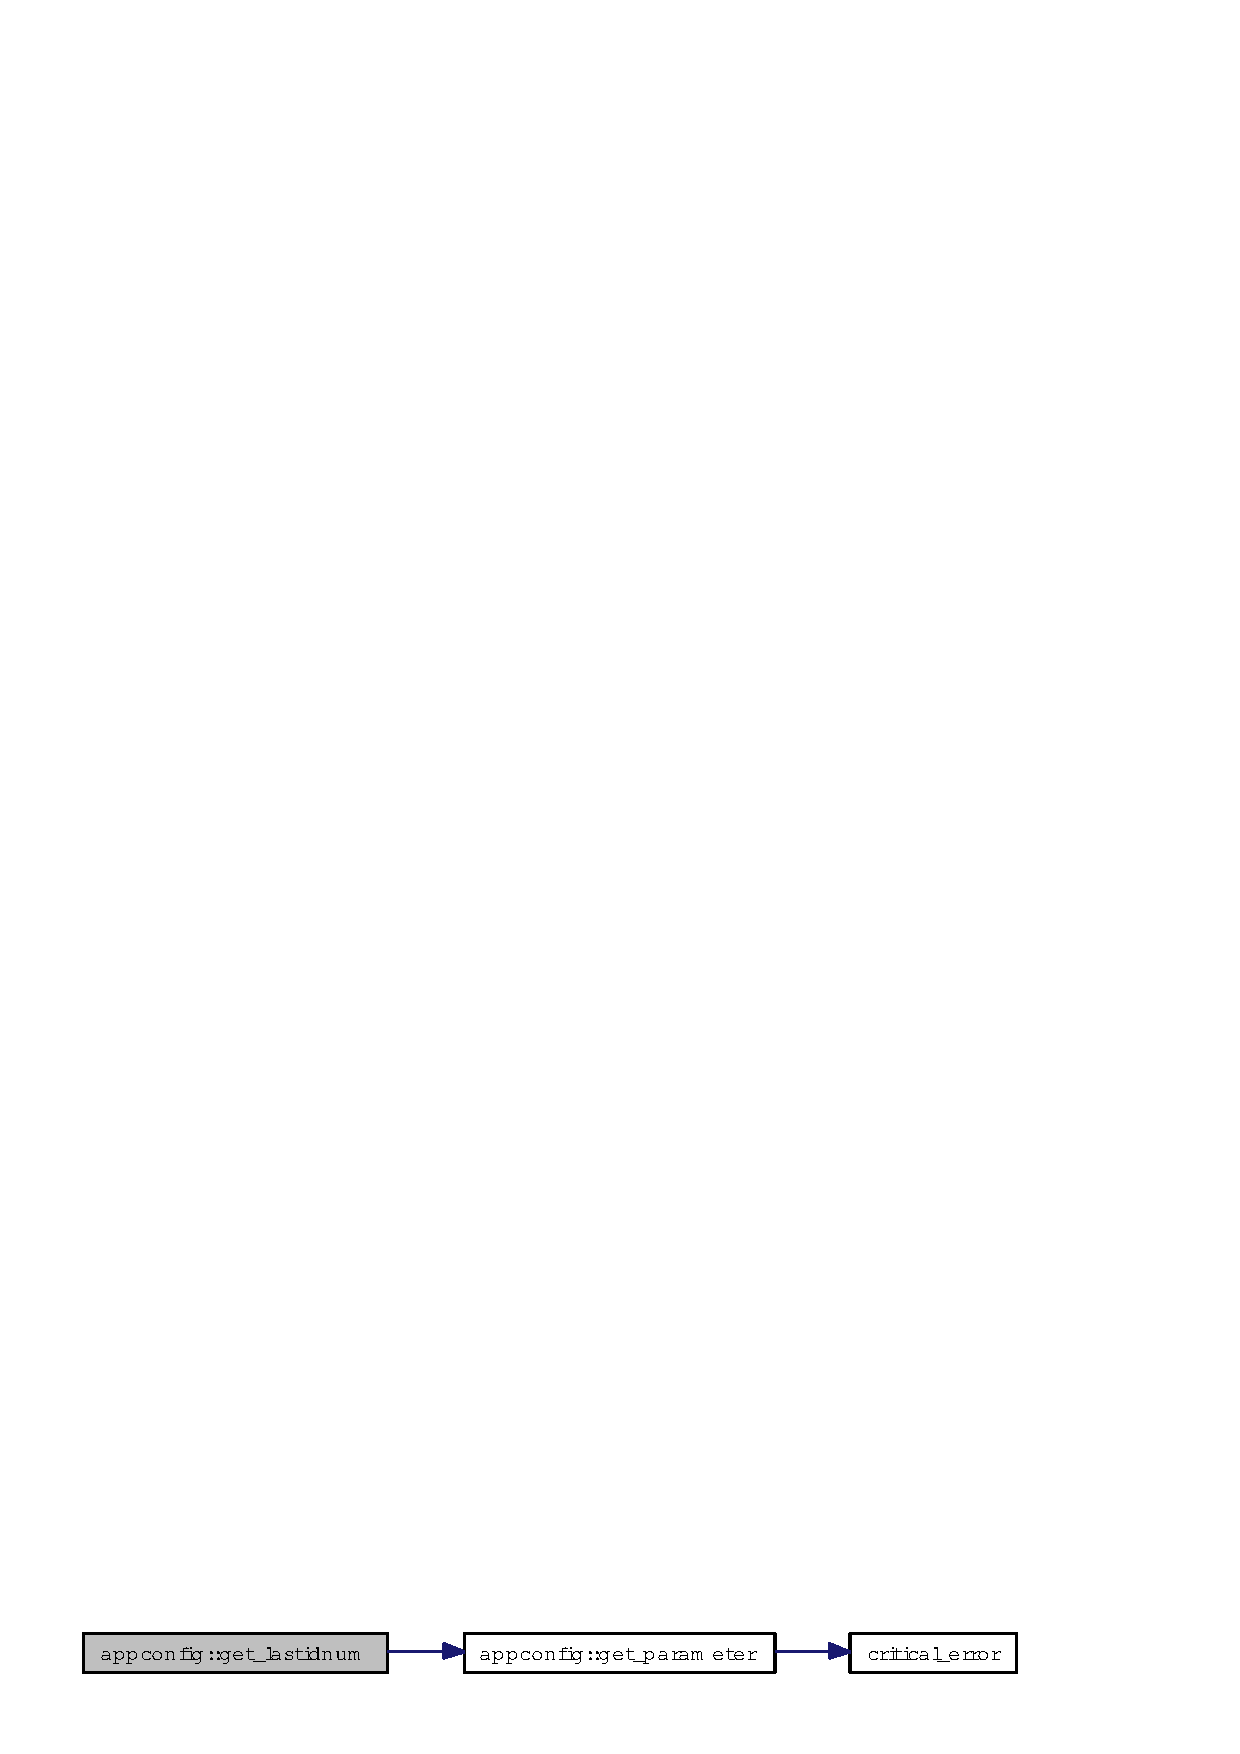
\includegraphics[width=246pt]{classappconfig_098e273bf84b2ce0ffcf69ce98d99acb_cgraph}
\end{center}
\end{figure}


Here is the caller graph for this function:\begin{figure}[H]
\begin{center}
\leavevmode
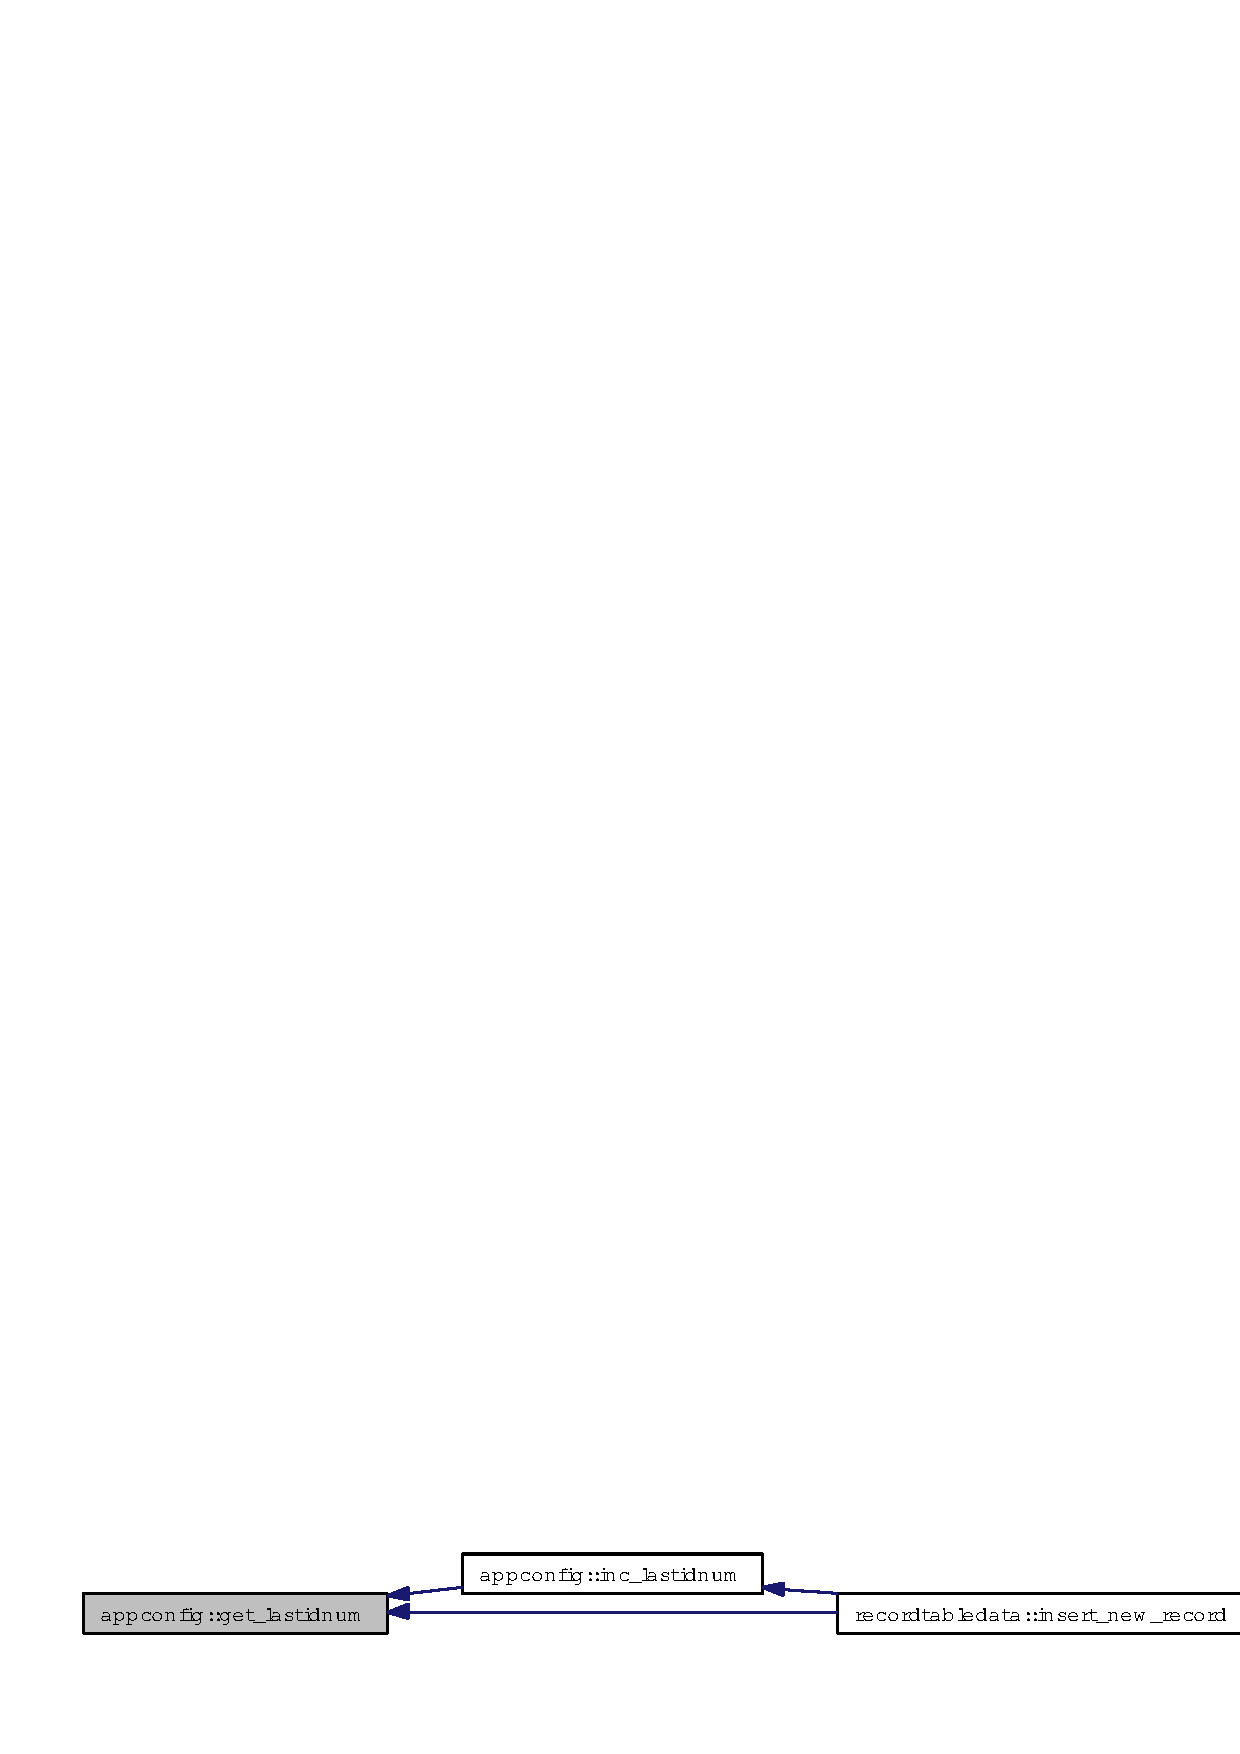
\includegraphics[width=399pt]{classappconfig_098e273bf84b2ce0ffcf69ce98d99acb_icgraph}
\end{center}
\end{figure}
\index{appconfig@{appconfig}!inc_lastidnum@{inc\_\-lastidnum}}
\index{inc_lastidnum@{inc\_\-lastidnum}!appconfig@{appconfig}}
\subsubsection{\setlength{\rightskip}{0pt plus 5cm}void appconfig::inc\_\-lastidnum (void)}\label{classappconfig_fe3089f67aa81ee6d5e8bd50dfe62e6b}




Definition at line 138 of file appconfig.cpp.

References conf, and get\_\-lastidnum().

Referenced by treescreen::ins\_\-branch(), treescreen::ins\_\-subbranch(), and recordtabledata::insert\_\-new\_\-record().

Here is the call graph for this function:\begin{figure}[H]
\begin{center}
\leavevmode
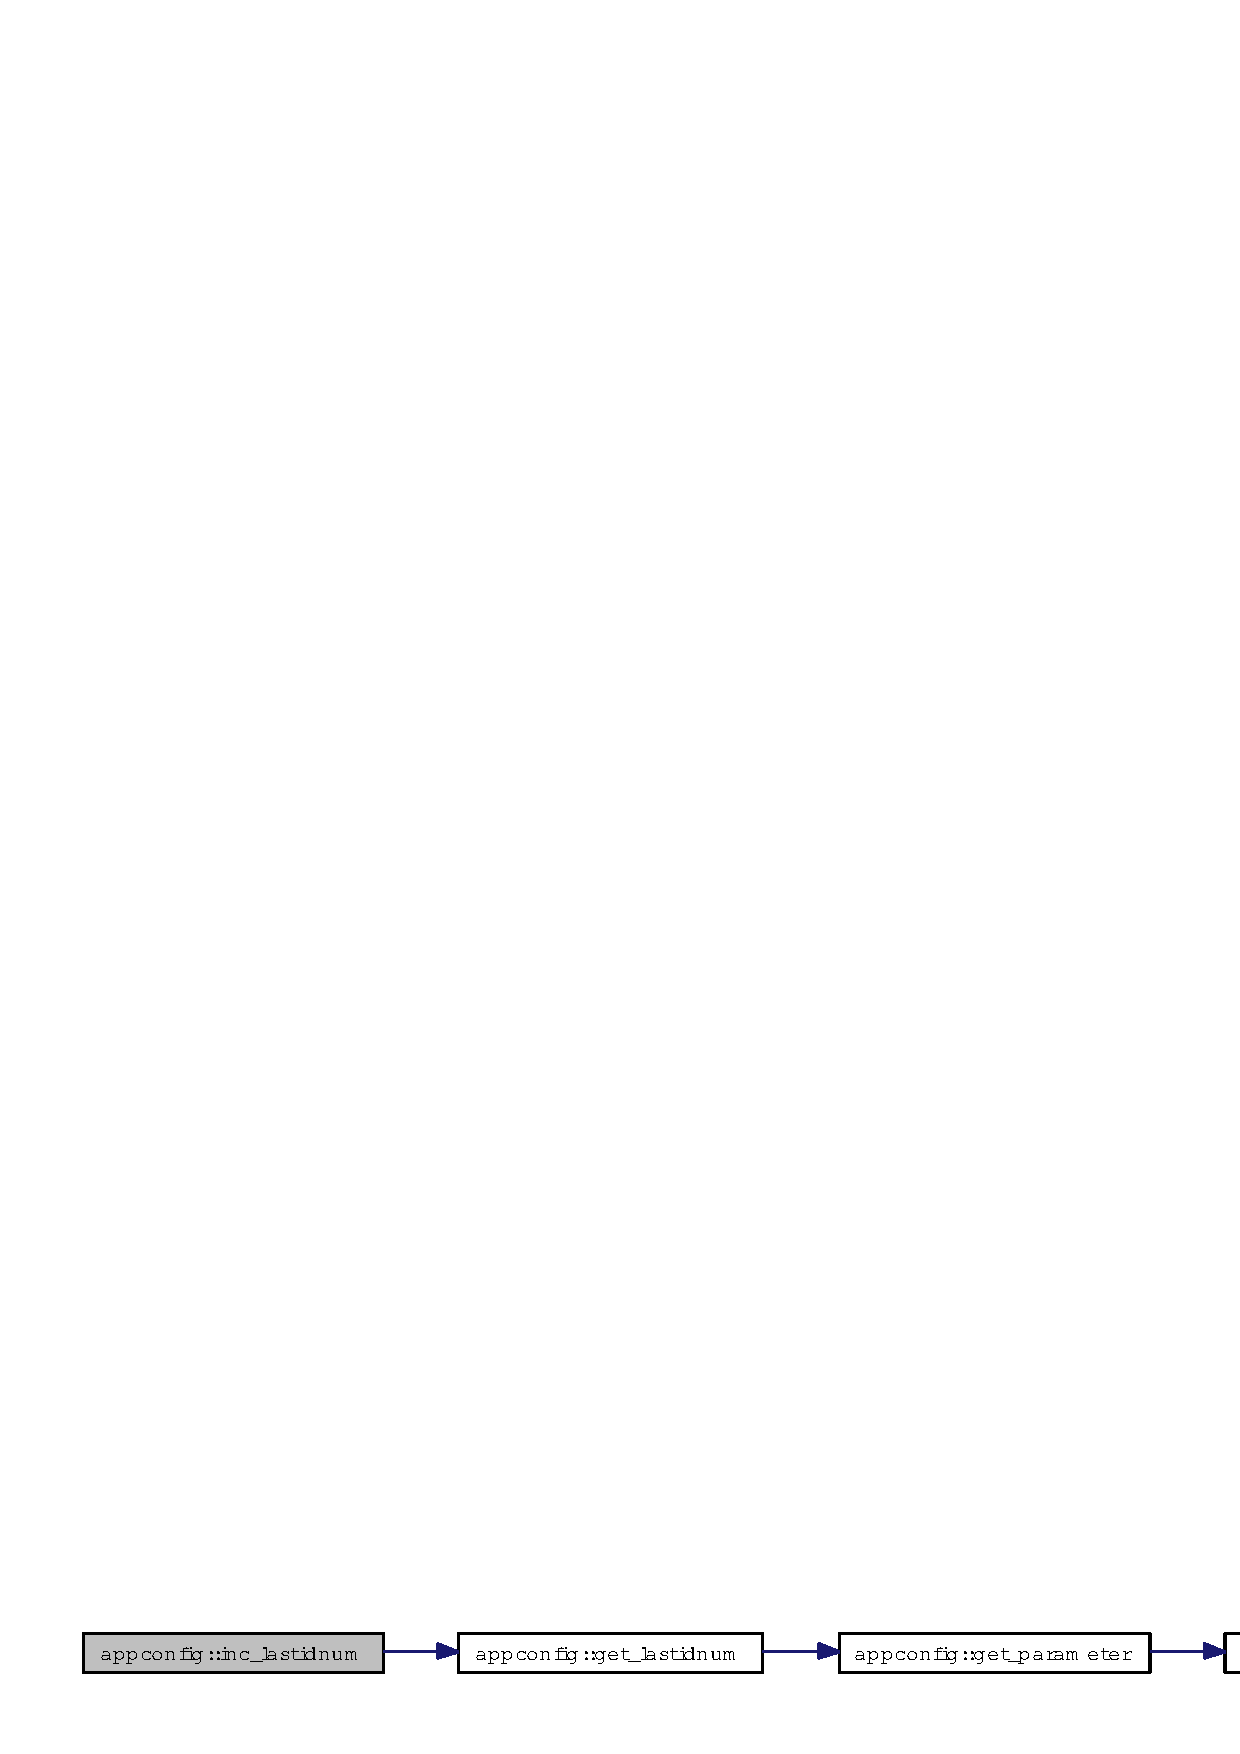
\includegraphics[width=336pt]{classappconfig_fe3089f67aa81ee6d5e8bd50dfe62e6b_cgraph}
\end{center}
\end{figure}


Here is the caller graph for this function:\begin{figure}[H]
\begin{center}
\leavevmode
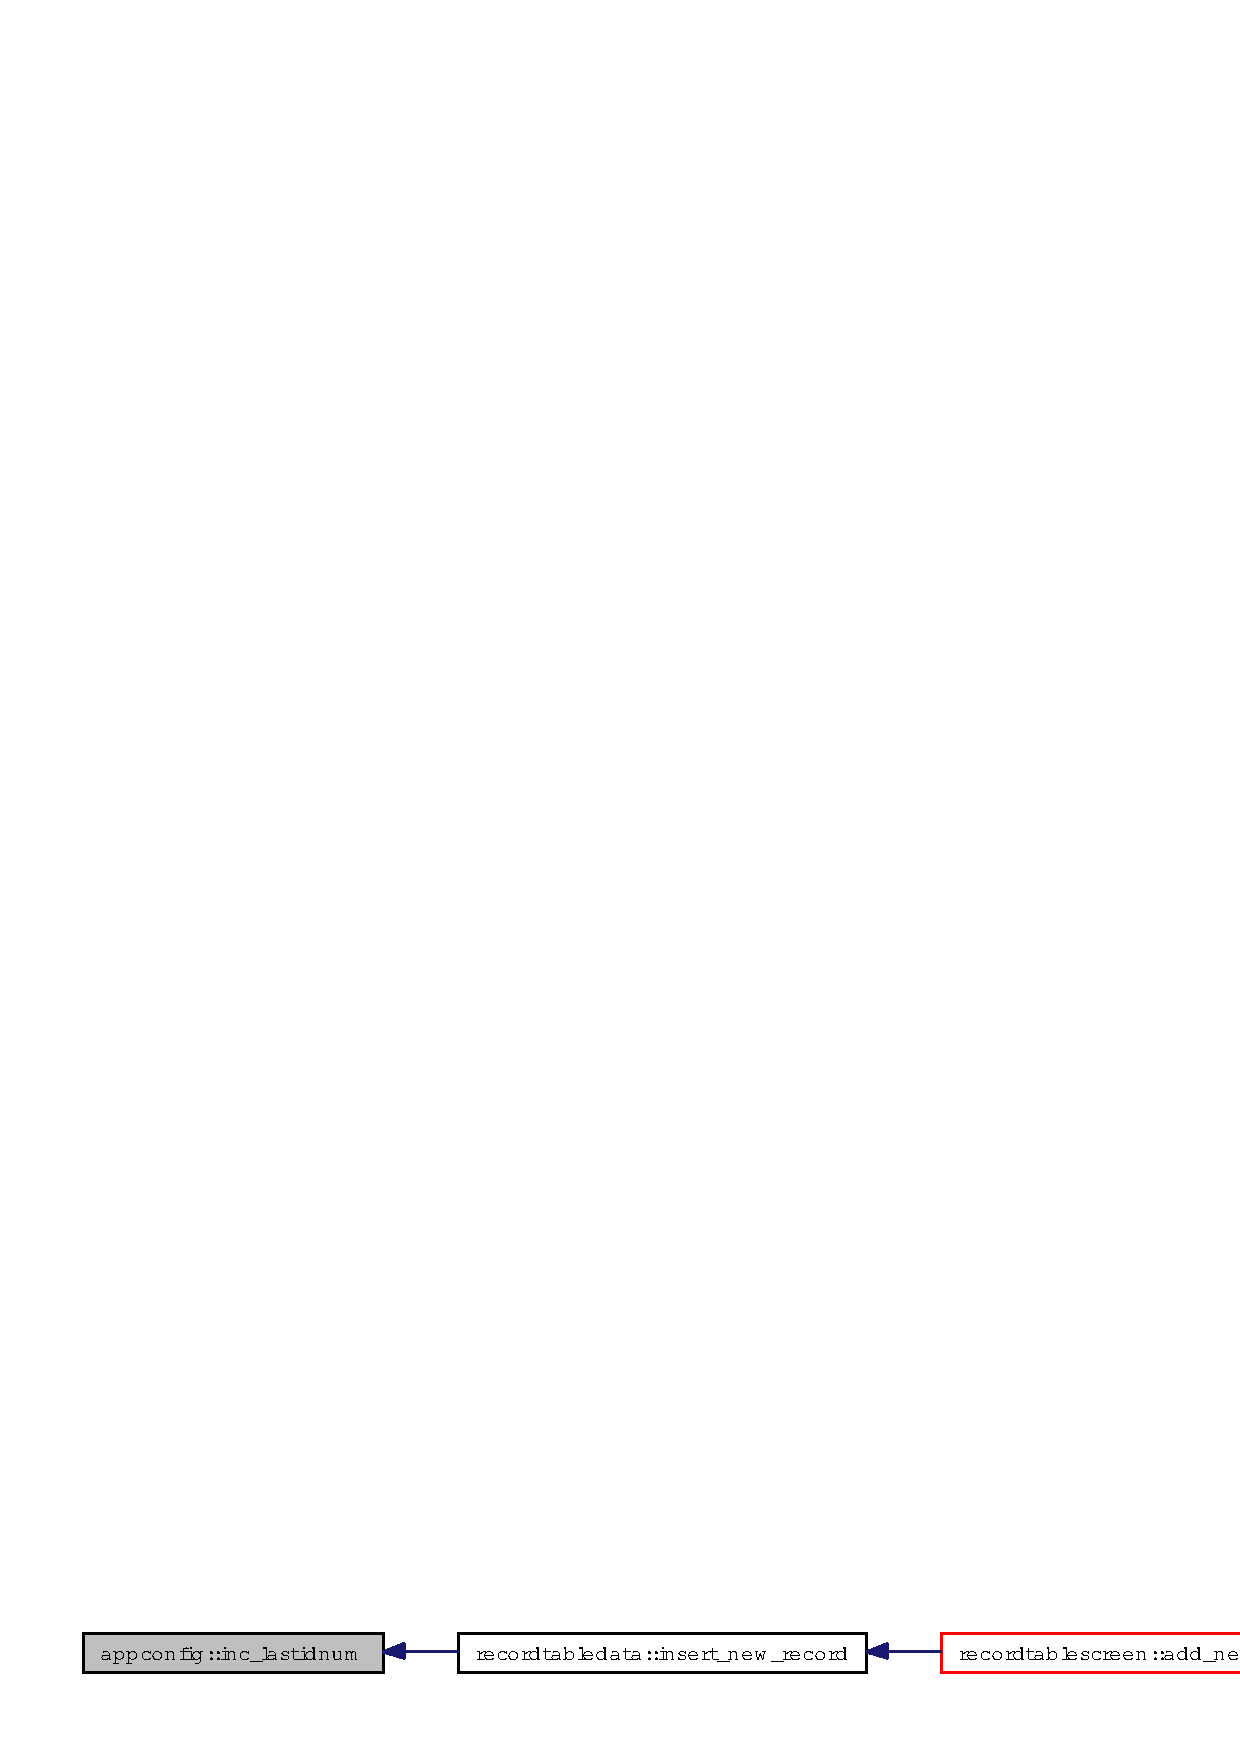
\includegraphics[width=308pt]{classappconfig_fe3089f67aa81ee6d5e8bd50dfe62e6b_icgraph}
\end{center}
\end{figure}
\index{appconfig@{appconfig}!get_lastprefixnum@{get\_\-lastprefixnum}}
\index{get_lastprefixnum@{get\_\-lastprefixnum}!appconfig@{appconfig}}
\subsubsection{\setlength{\rightskip}{0pt plus 5cm}int appconfig::get\_\-lastprefixnum (void)}\label{classappconfig_3432611171d82a5597bed8102d3590dd}




Definition at line 150 of file appconfig.cpp.

References get\_\-parameter().

Referenced by inc\_\-lastprefixnum().

Here is the call graph for this function:\begin{figure}[H]
\begin{center}
\leavevmode
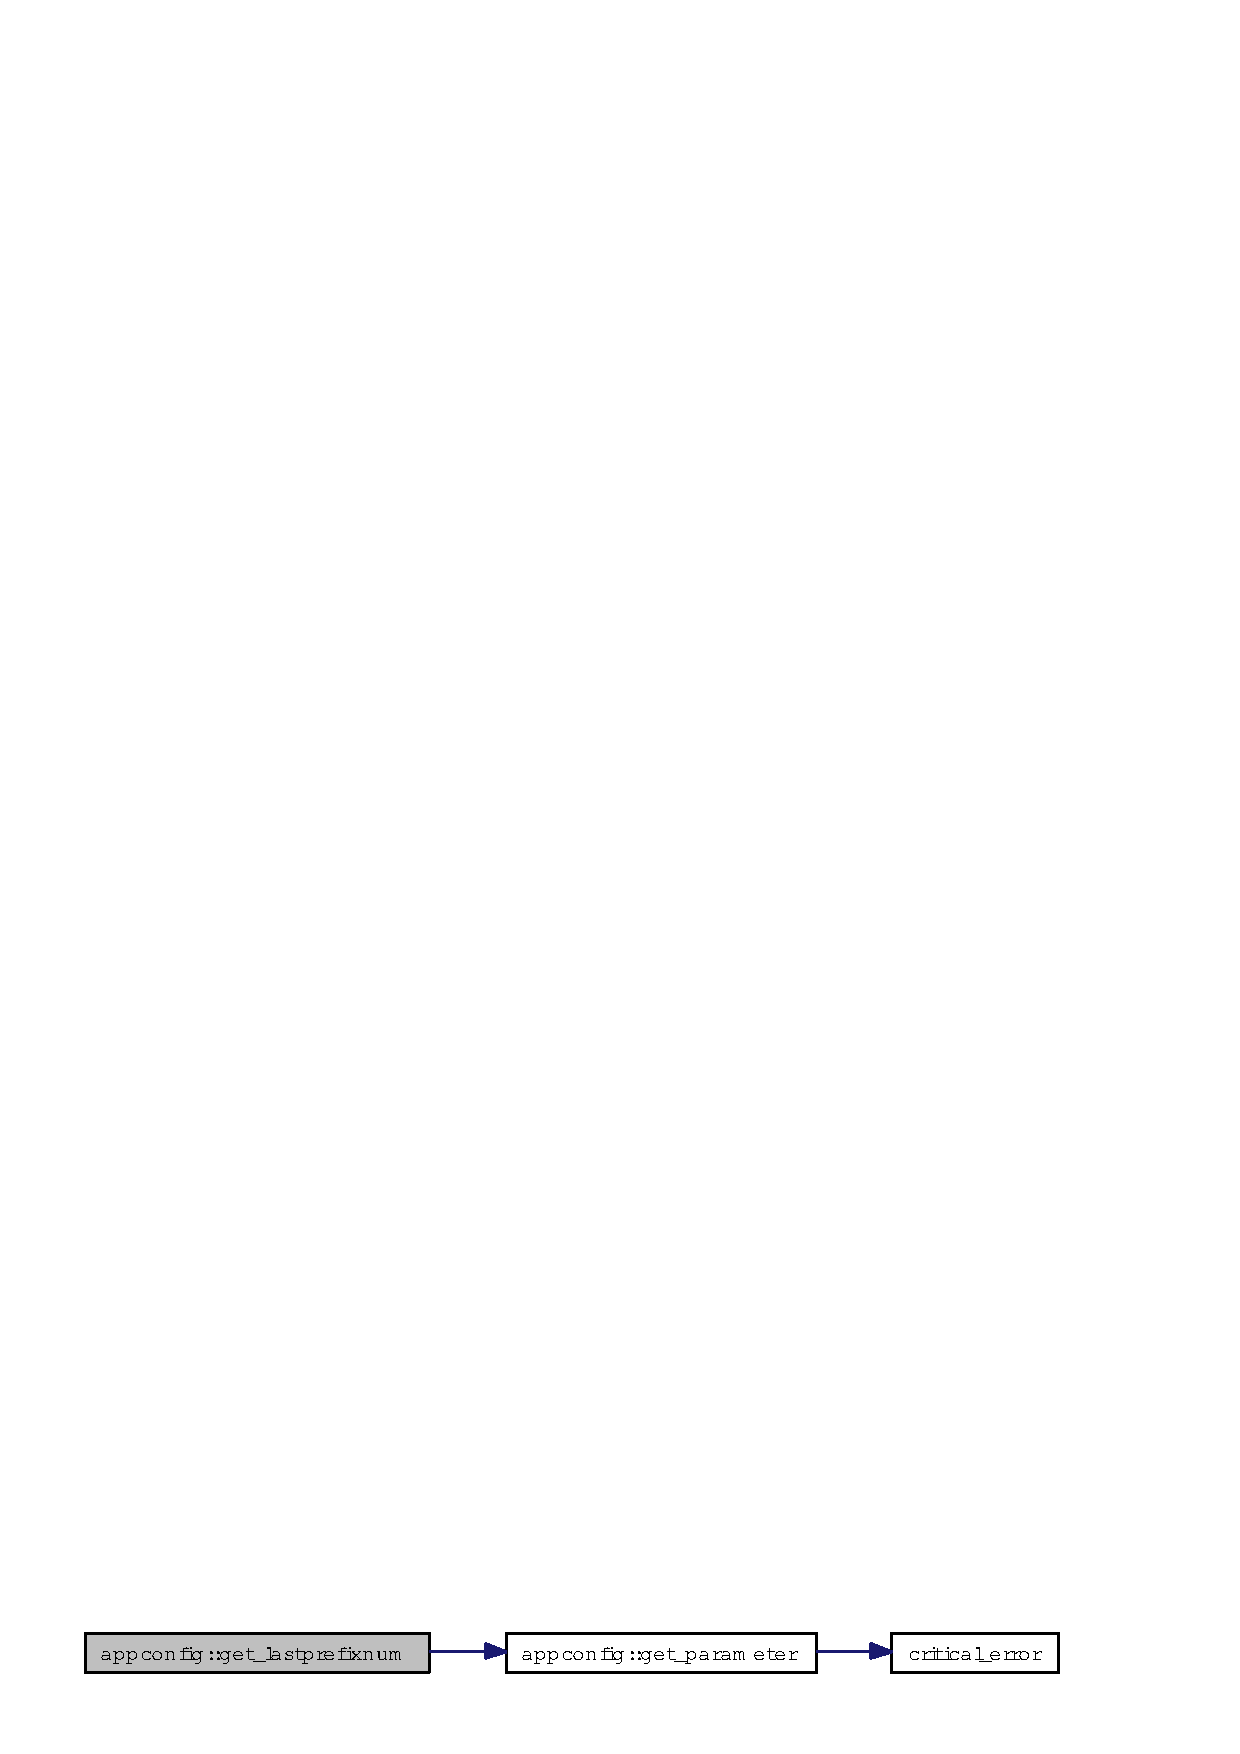
\includegraphics[width=256pt]{classappconfig_3432611171d82a5597bed8102d3590dd_cgraph}
\end{center}
\end{figure}


Here is the caller graph for this function:\begin{figure}[H]
\begin{center}
\leavevmode
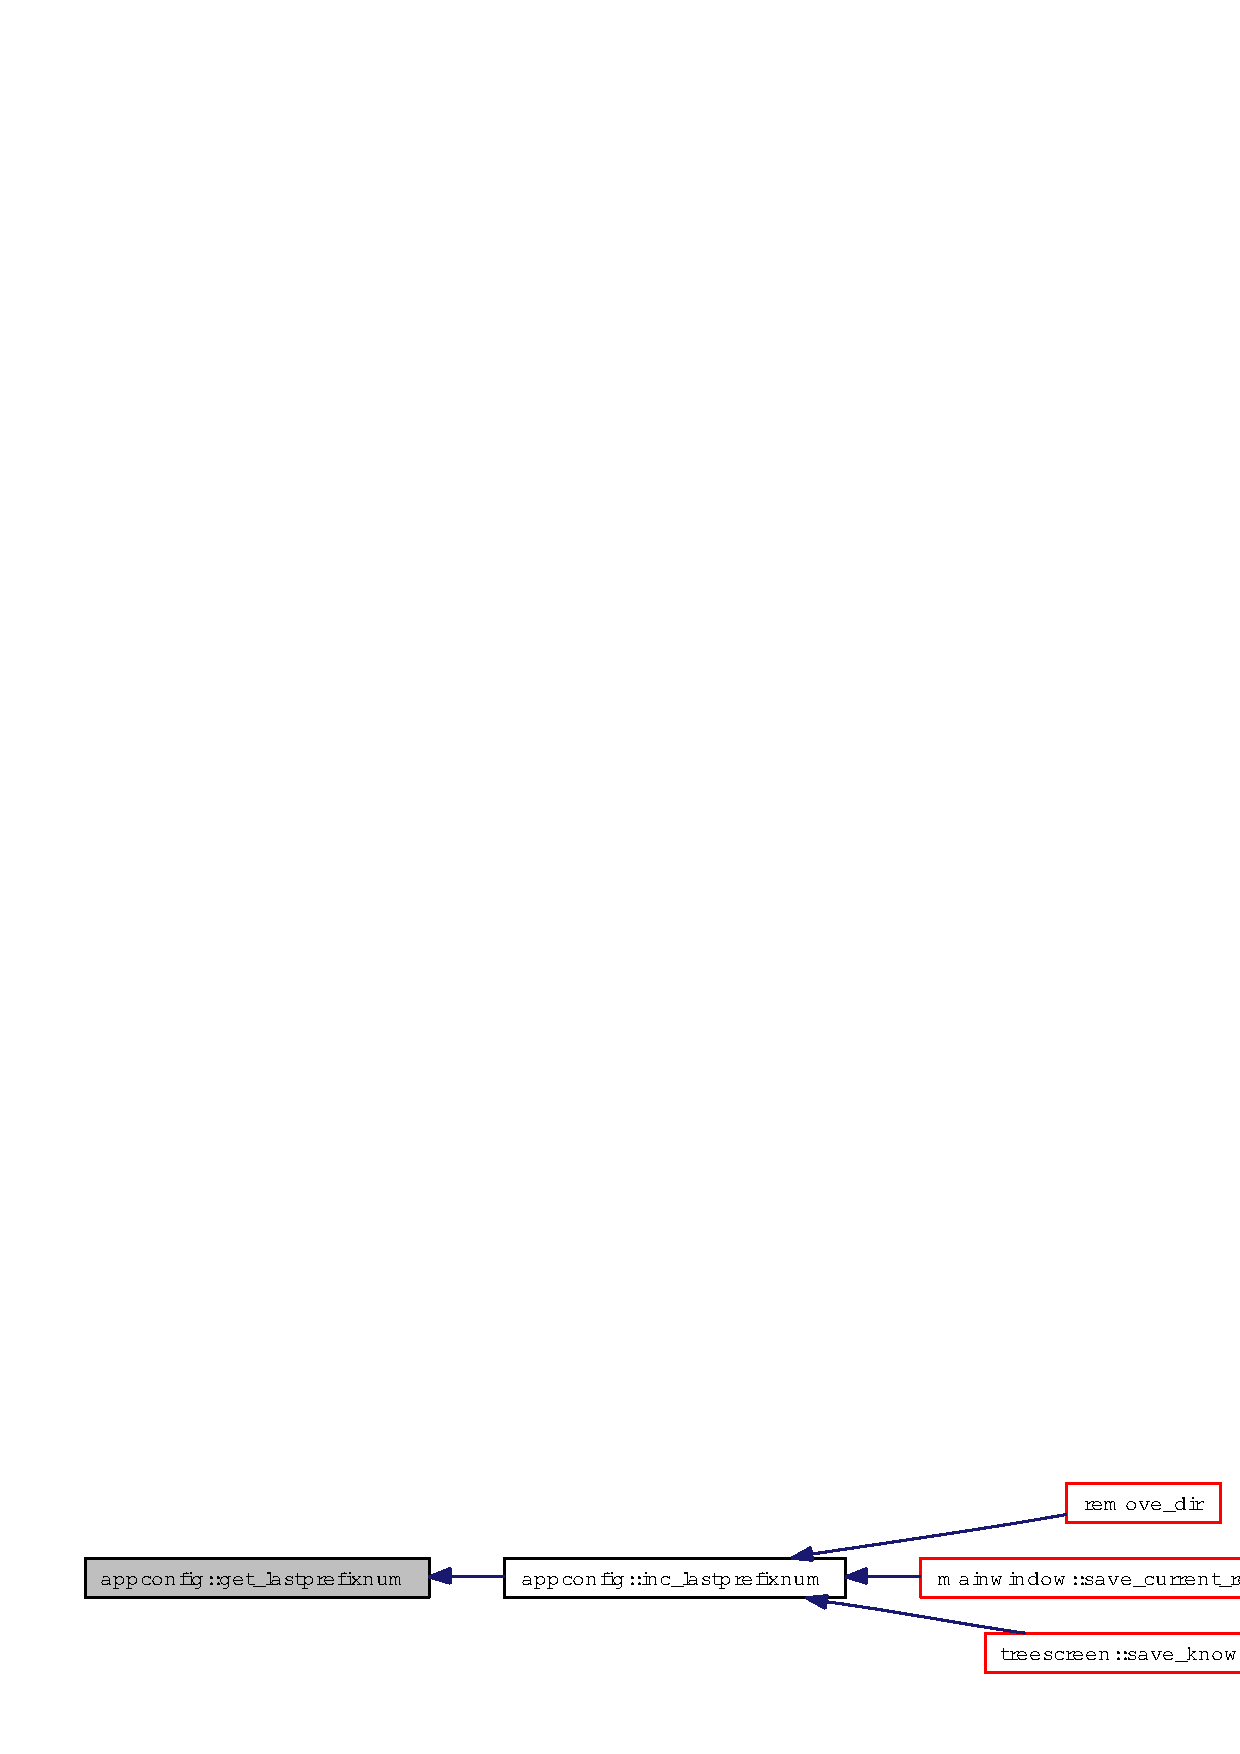
\includegraphics[width=330pt]{classappconfig_3432611171d82a5597bed8102d3590dd_icgraph}
\end{center}
\end{figure}
\index{appconfig@{appconfig}!get_lastprefixnum_as_line@{get\_\-lastprefixnum\_\-as\_\-line}}
\index{get_lastprefixnum_as_line@{get\_\-lastprefixnum\_\-as\_\-line}!appconfig@{appconfig}}
\subsubsection{\setlength{\rightskip}{0pt plus 5cm}QString appconfig::get\_\-lastprefixnum\_\-as\_\-line (void)}\label{classappconfig_fdf2d9c2c13bfd05de4e7dad69ed5614}




Definition at line 162 of file appconfig.cpp.

References get\_\-parameter().

Referenced by remove\_\-dir(), mainwindow::save\_\-current\_\-record\_\-text(), and treescreen::save\_\-knowtree().

Here is the call graph for this function:\begin{figure}[H]
\begin{center}
\leavevmode
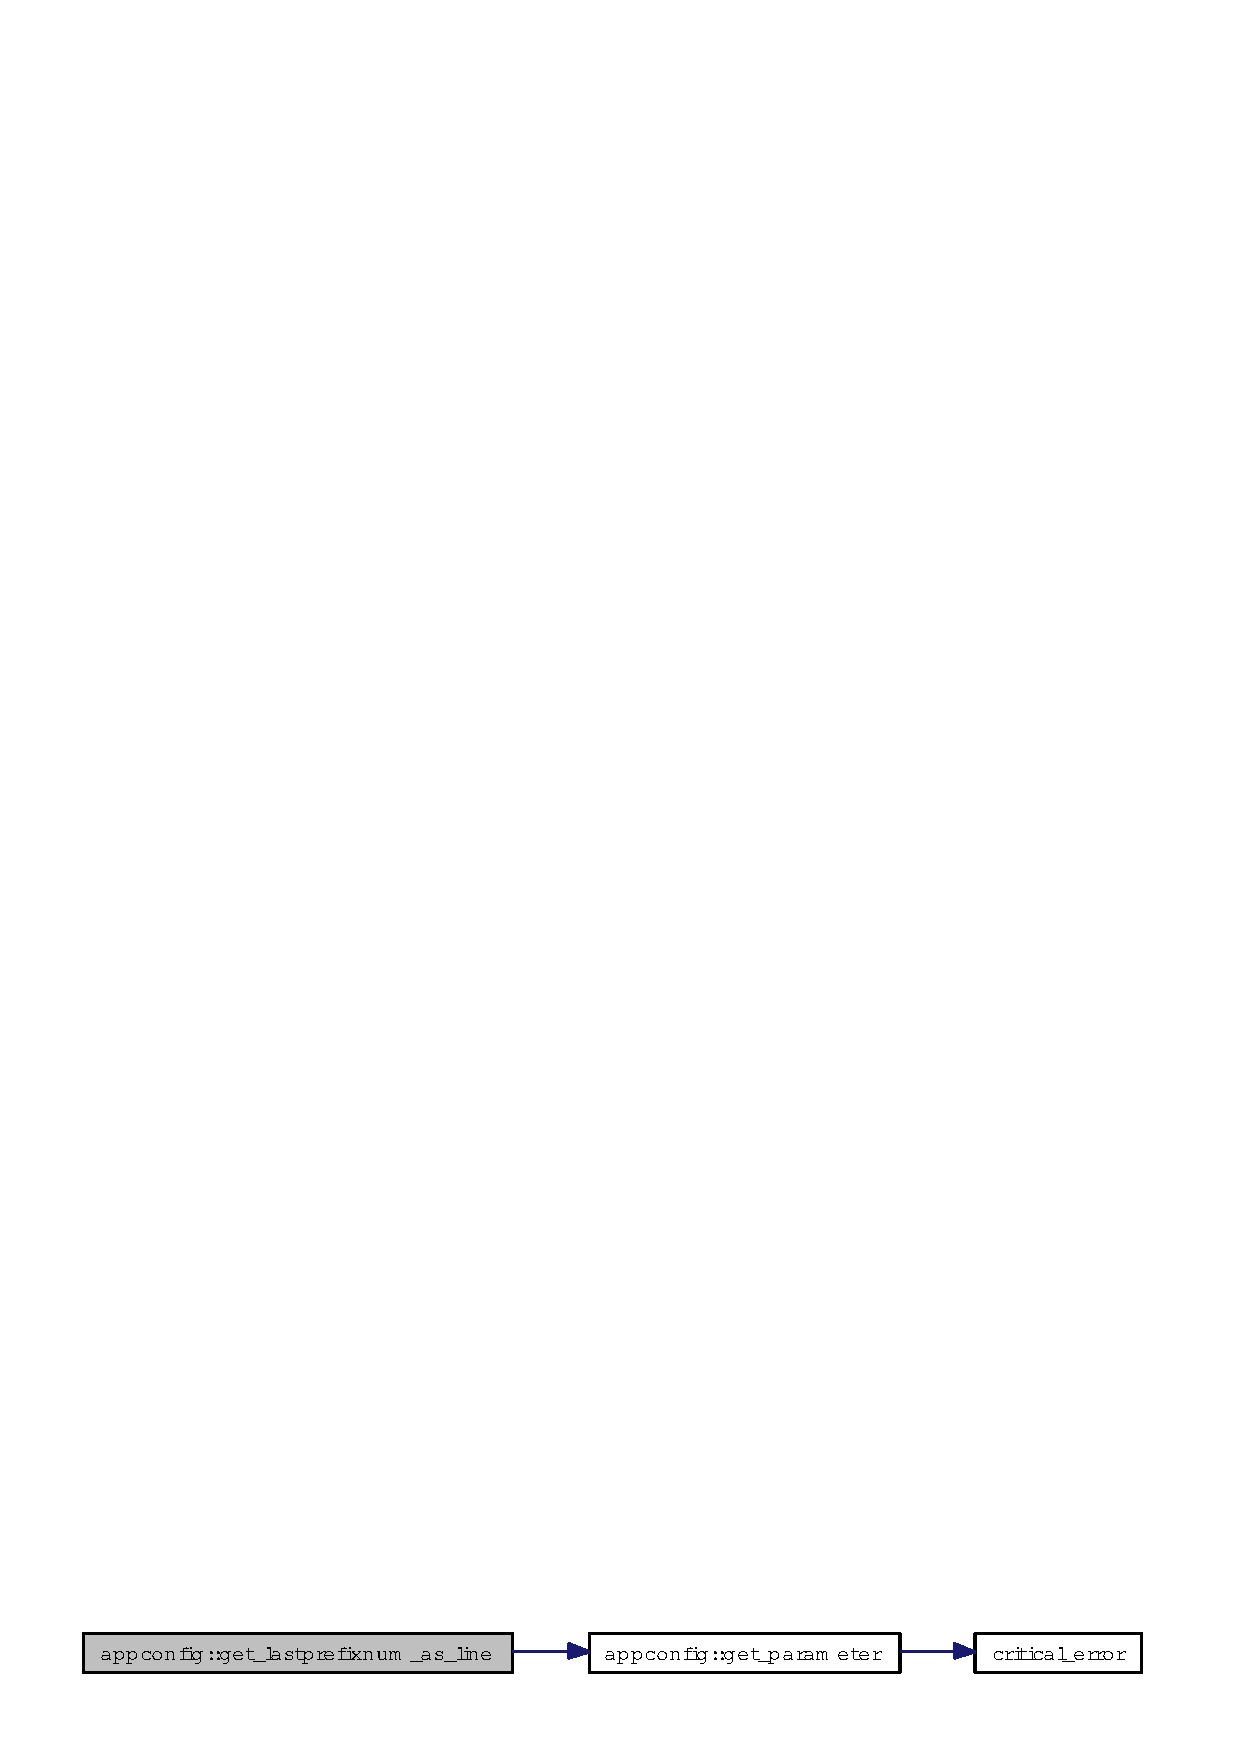
\includegraphics[width=276pt]{classappconfig_fdf2d9c2c13bfd05de4e7dad69ed5614_cgraph}
\end{center}
\end{figure}


Here is the caller graph for this function:\begin{figure}[H]
\begin{center}
\leavevmode
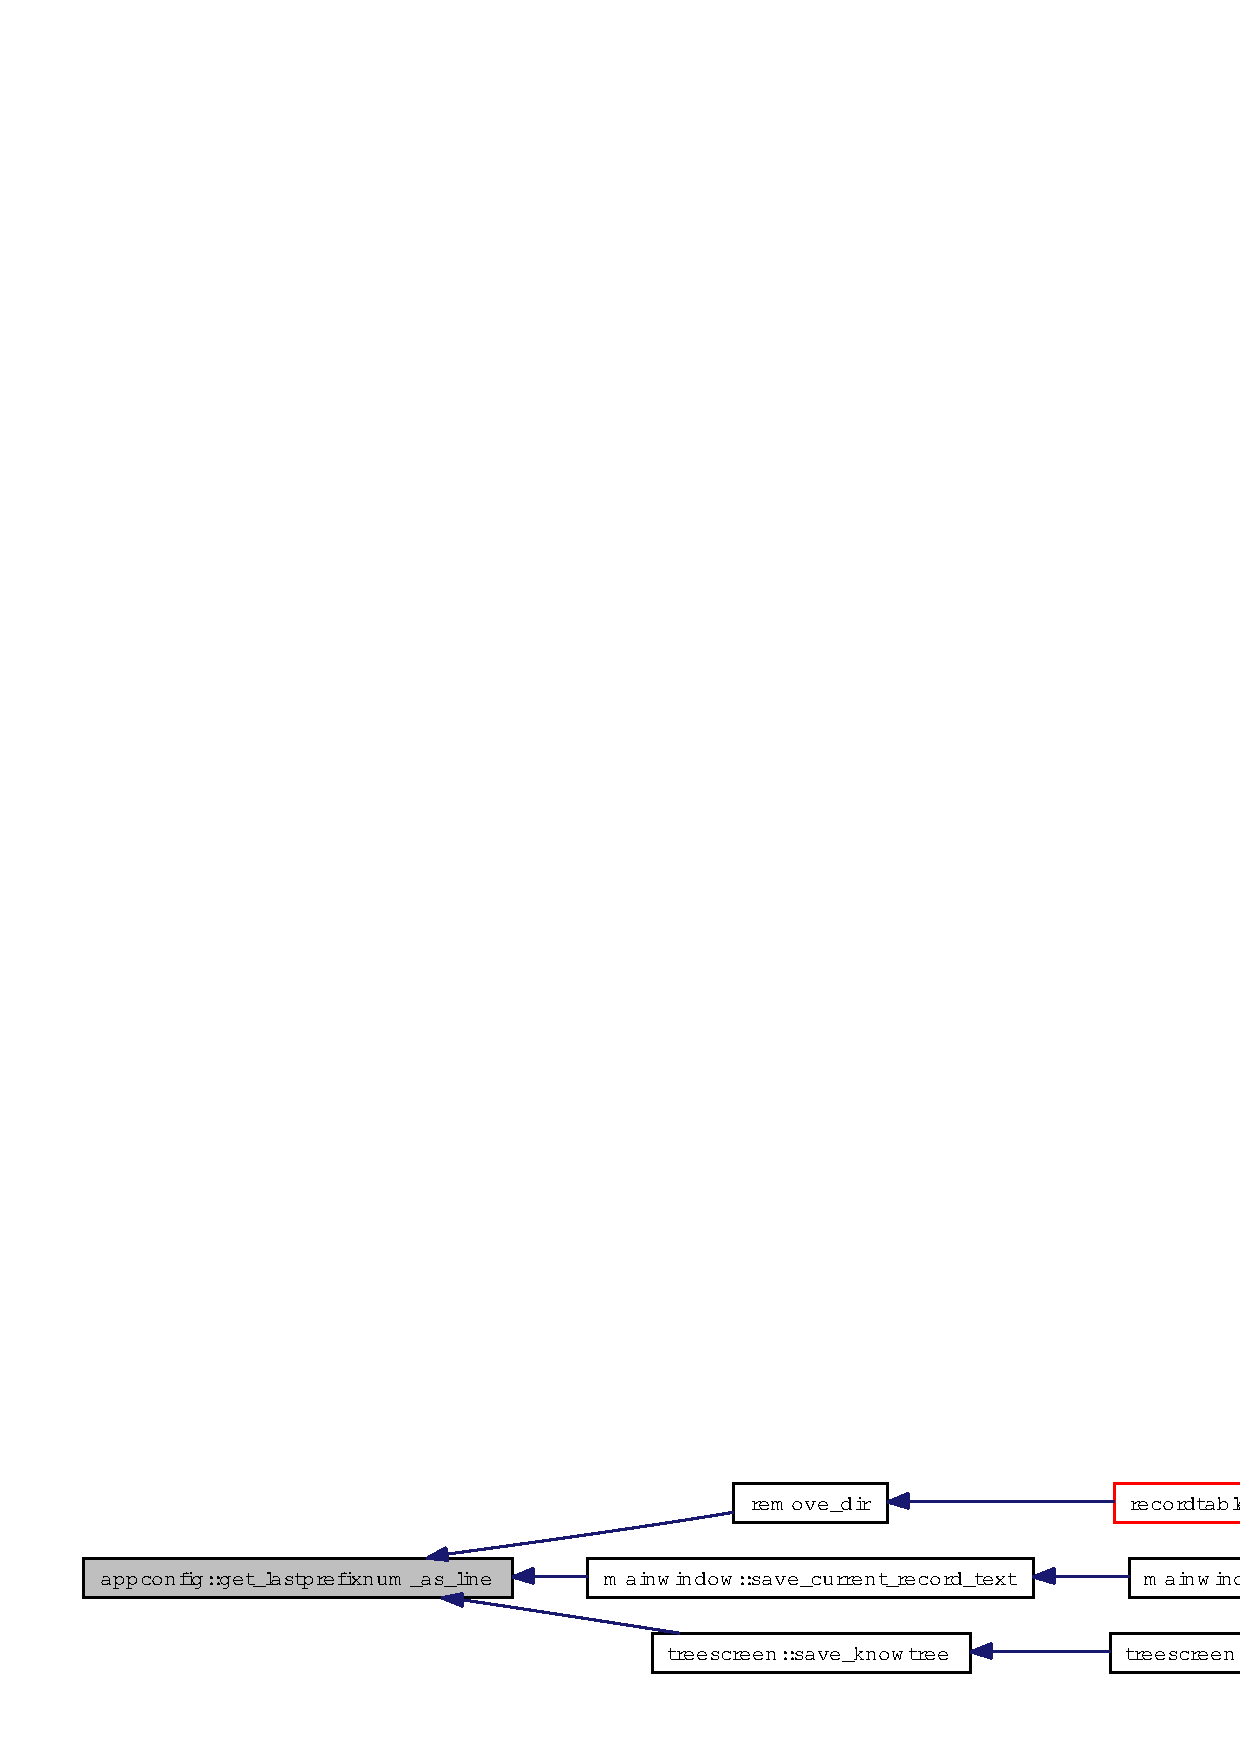
\includegraphics[width=357pt]{classappconfig_fdf2d9c2c13bfd05de4e7dad69ed5614_icgraph}
\end{center}
\end{figure}
\index{appconfig@{appconfig}!inc_lastprefixnum@{inc\_\-lastprefixnum}}
\index{inc_lastprefixnum@{inc\_\-lastprefixnum}!appconfig@{appconfig}}
\subsubsection{\setlength{\rightskip}{0pt plus 5cm}void appconfig::inc\_\-lastprefixnum (void)}\label{classappconfig_f96423b10ba9101a88de147b1f4fe7bb}




Definition at line 173 of file appconfig.cpp.

References conf, and get\_\-lastprefixnum().

Referenced by remove\_\-dir(), mainwindow::save\_\-current\_\-record\_\-text(), and treescreen::save\_\-knowtree().

Here is the call graph for this function:\begin{figure}[H]
\begin{center}
\leavevmode
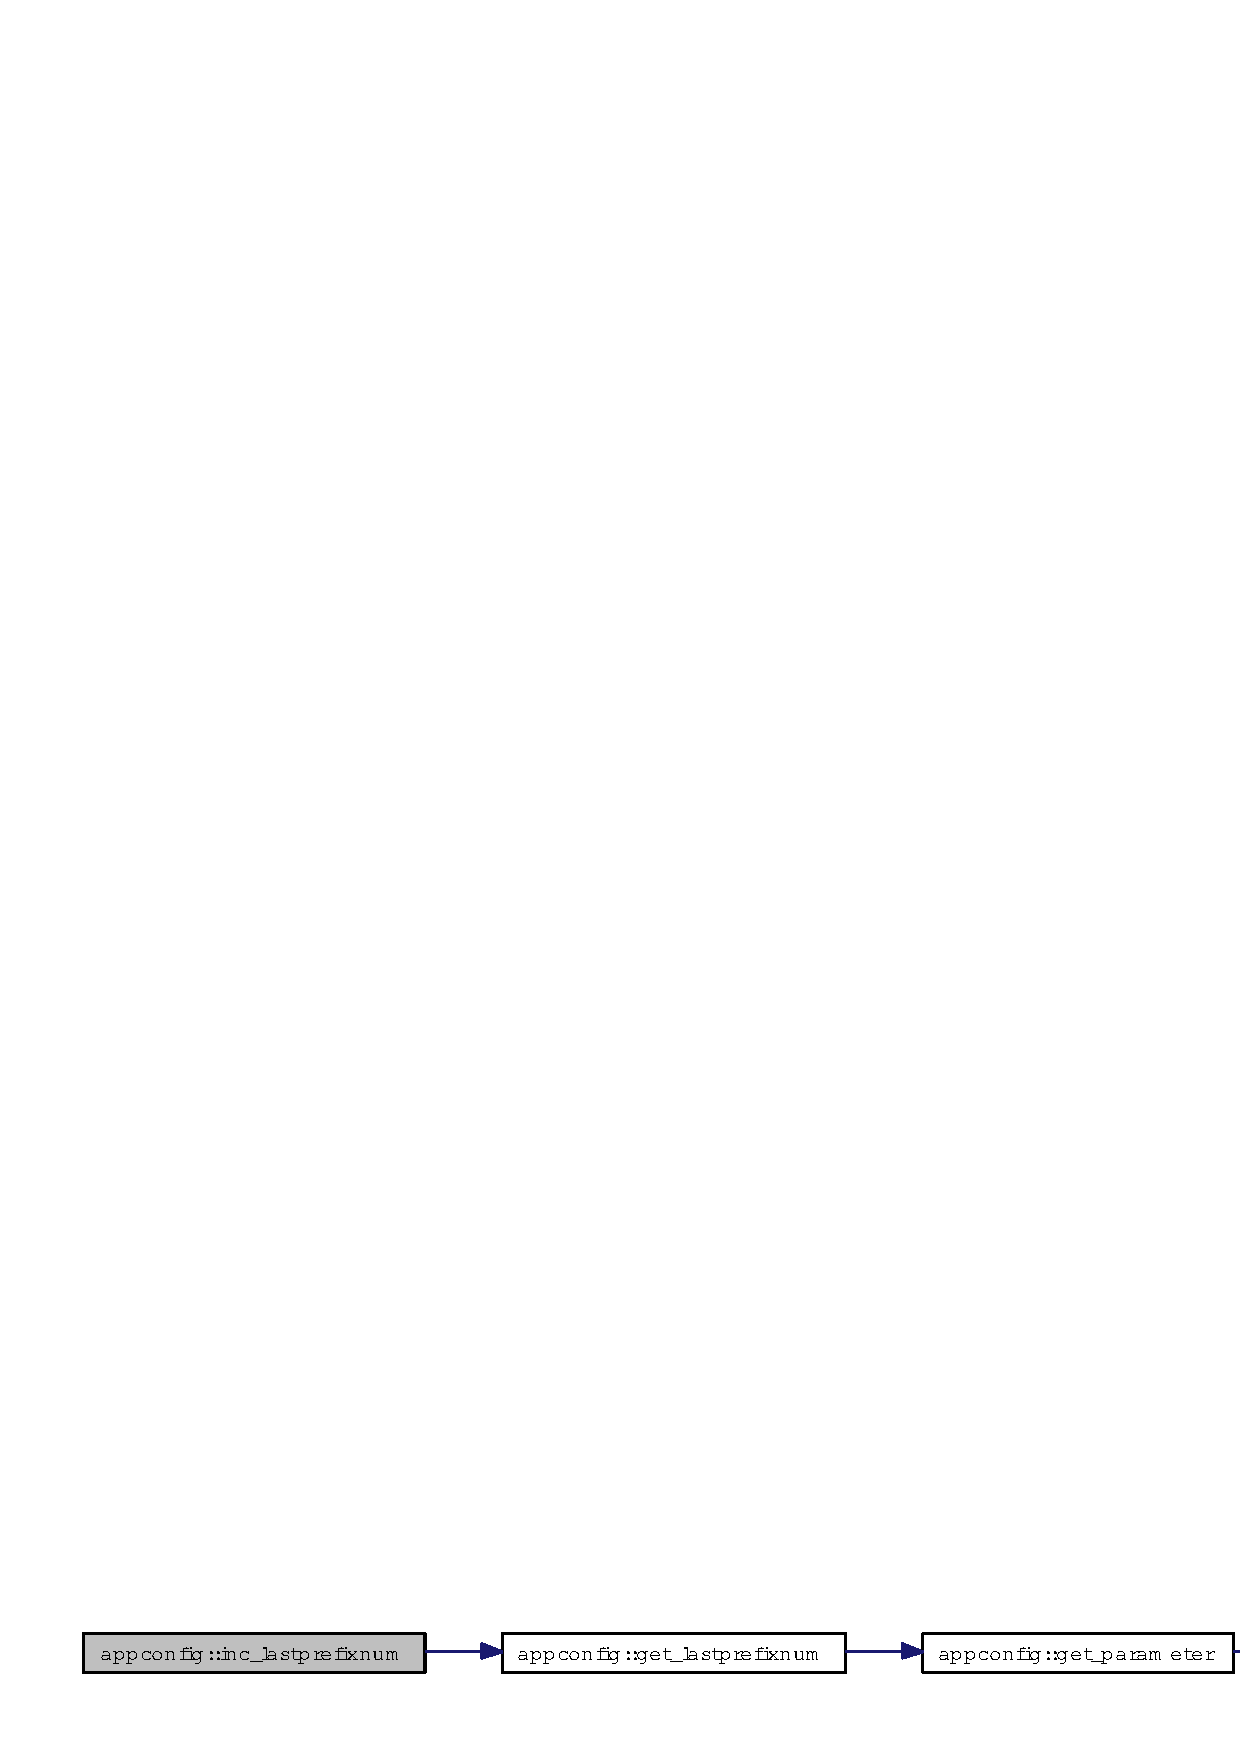
\includegraphics[width=356pt]{classappconfig_f96423b10ba9101a88de147b1f4fe7bb_cgraph}
\end{center}
\end{figure}


Here is the caller graph for this function:\begin{figure}[H]
\begin{center}
\leavevmode
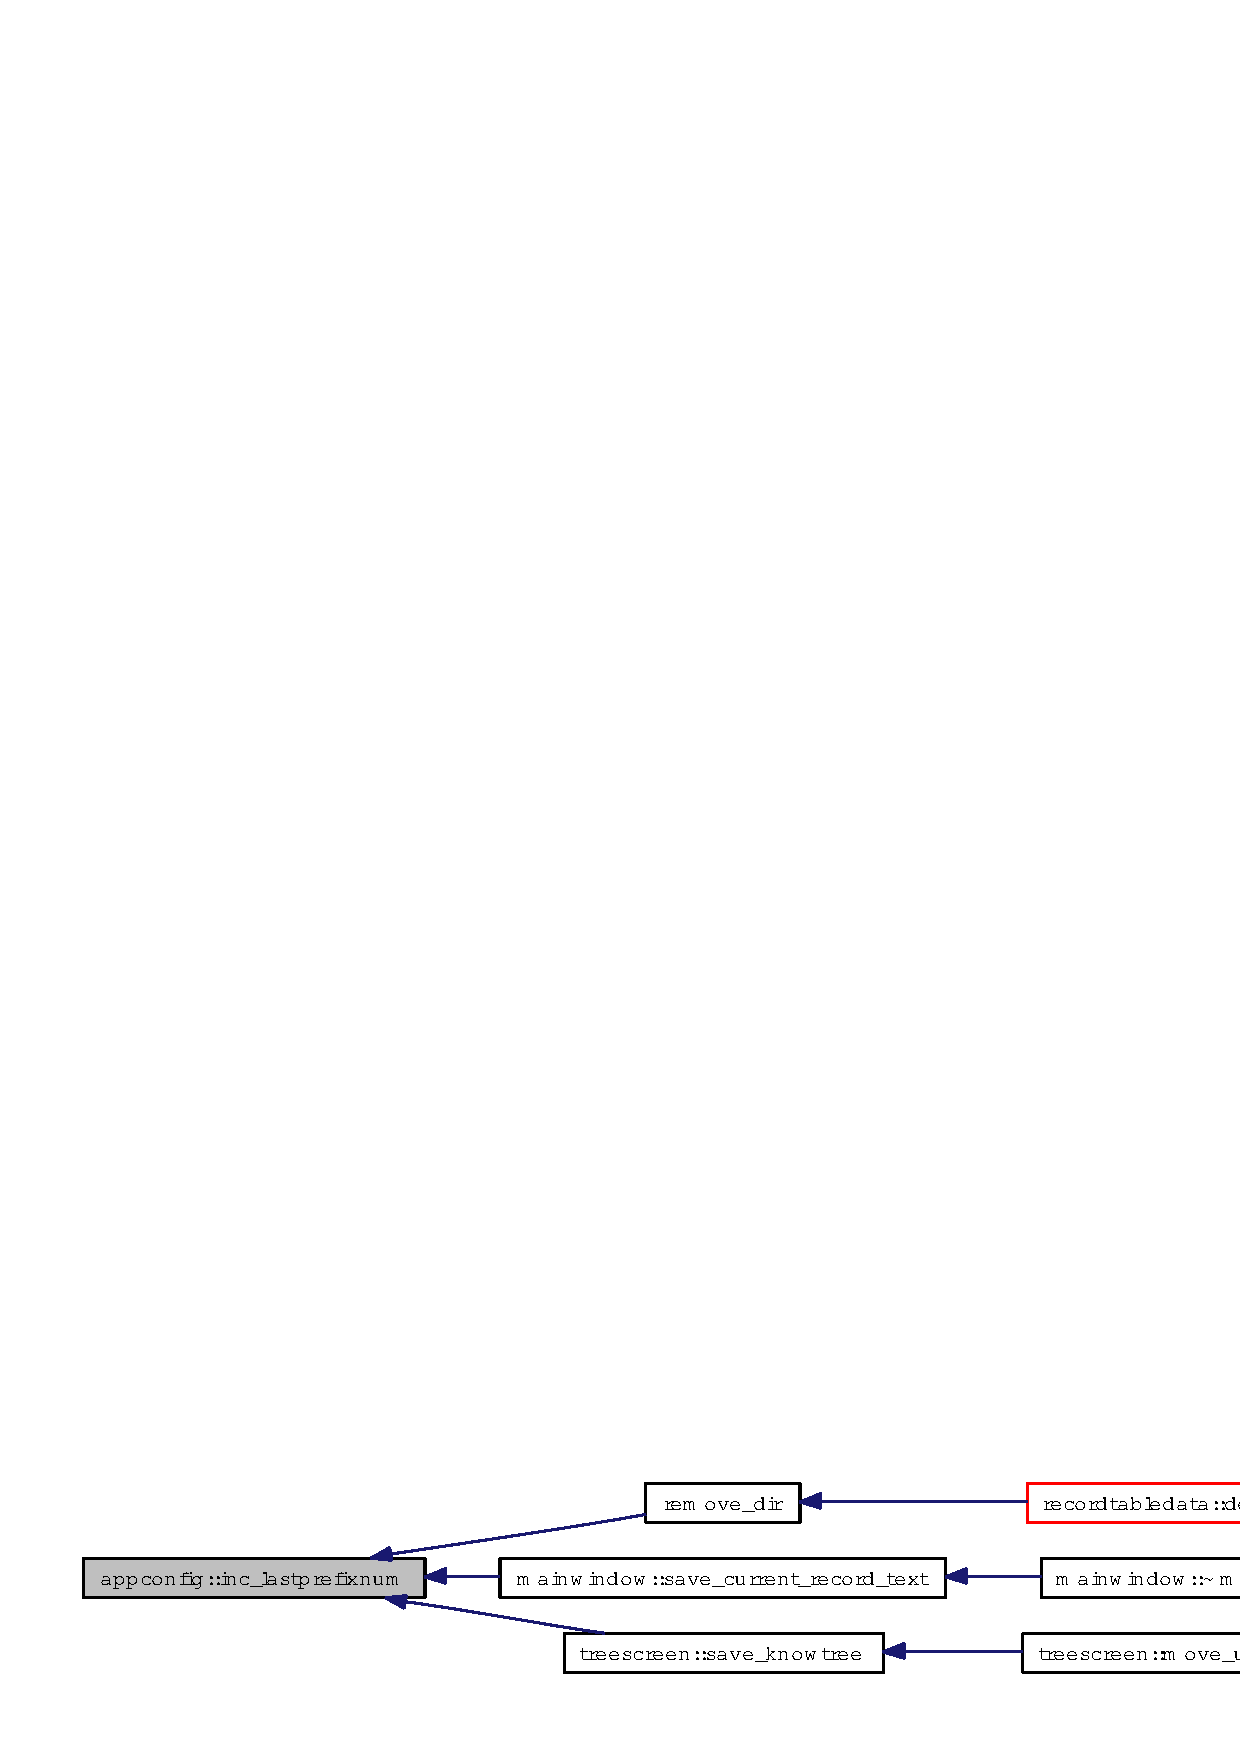
\includegraphics[width=336pt]{classappconfig_f96423b10ba9101a88de147b1f4fe7bb_icgraph}
\end{center}
\end{figure}
\index{appconfig@{appconfig}!get_addnewrecord_expand_info@{get\_\-addnewrecord\_\-expand\_\-info}}
\index{get_addnewrecord_expand_info@{get\_\-addnewrecord\_\-expand\_\-info}!appconfig@{appconfig}}
\subsubsection{\setlength{\rightskip}{0pt plus 5cm}QString appconfig::get\_\-addnewrecord\_\-expand\_\-info (void)}\label{classappconfig_5e3fa8839799f2622089946d29a359c8}




Definition at line 183 of file appconfig.cpp.

References get\_\-parameter().

Referenced by infofieldenter::assembly(), infofieldenter::expand\_\-info\_\-click(), and infofieldenter::setup\_\-ui().

Here is the call graph for this function:\begin{figure}[H]
\begin{center}
\leavevmode
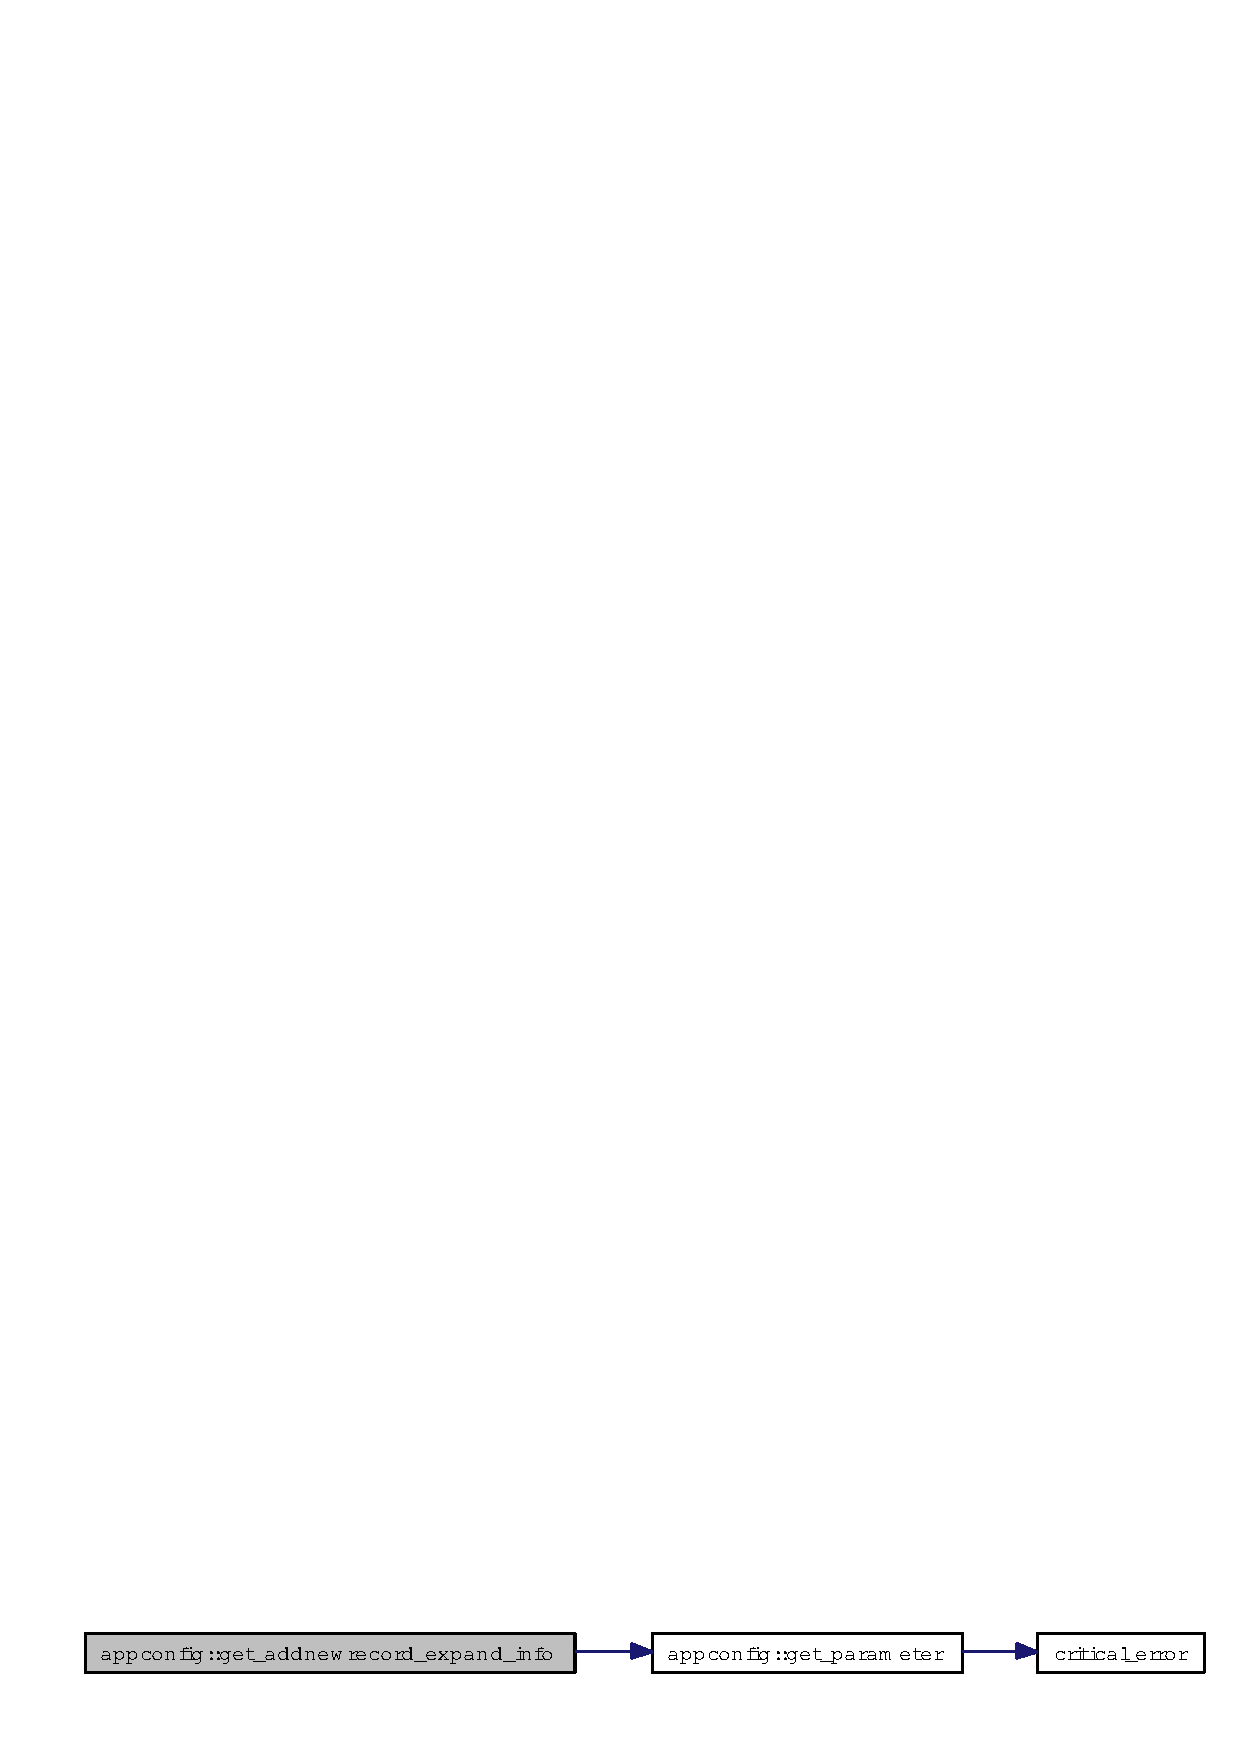
\includegraphics[width=291pt]{classappconfig_5e3fa8839799f2622089946d29a359c8_cgraph}
\end{center}
\end{figure}


Here is the caller graph for this function:\begin{figure}[H]
\begin{center}
\leavevmode
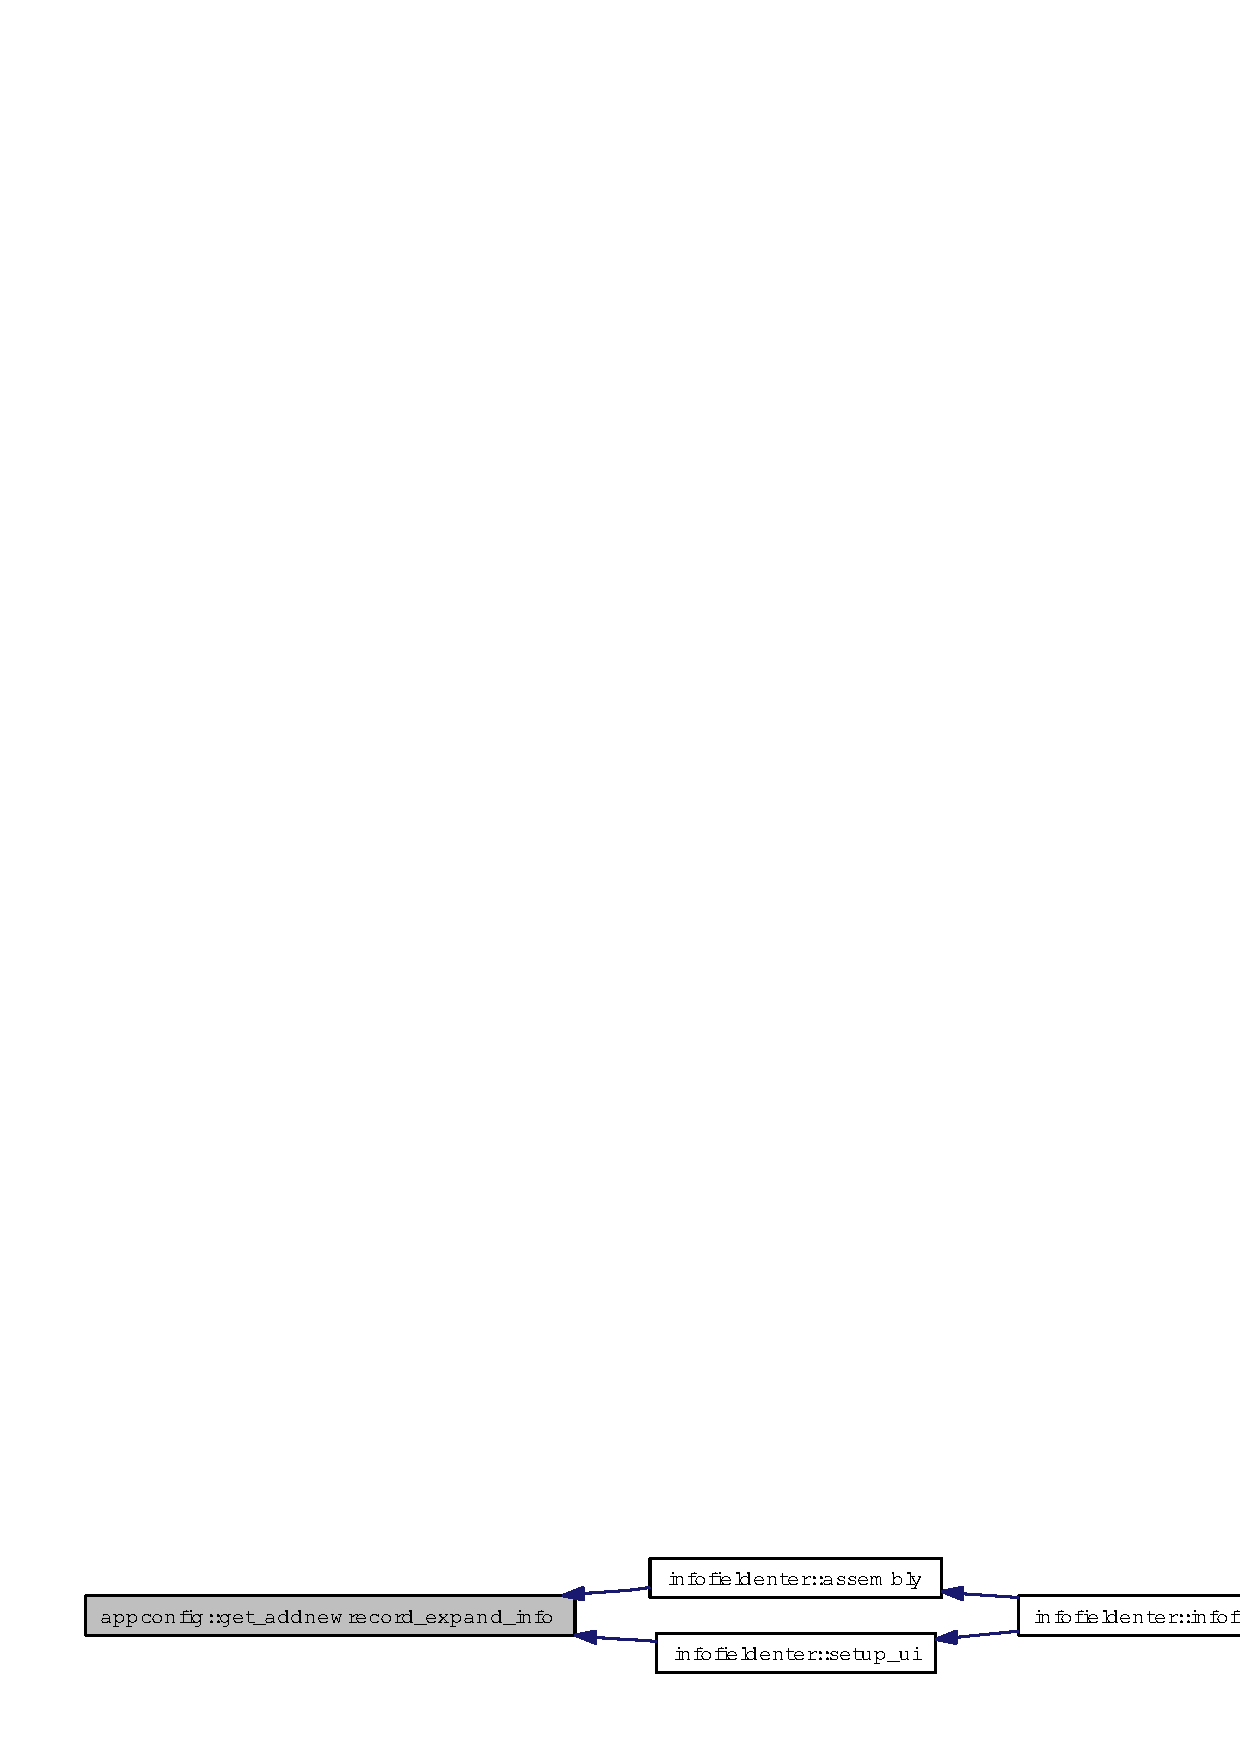
\includegraphics[width=326pt]{classappconfig_5e3fa8839799f2622089946d29a359c8_icgraph}
\end{center}
\end{figure}
\index{appconfig@{appconfig}!set_addnewrecord_expand_info@{set\_\-addnewrecord\_\-expand\_\-info}}
\index{set_addnewrecord_expand_info@{set\_\-addnewrecord\_\-expand\_\-info}!appconfig@{appconfig}}
\subsubsection{\setlength{\rightskip}{0pt plus 5cm}void appconfig::set\_\-addnewrecord\_\-expand\_\-info (QString)}\label{classappconfig_380f3e044a57a554dc2d7980a016a3e2}




Definition at line 188 of file appconfig.cpp.

References conf, and critical\_\-error().

Referenced by infofieldenter::expand\_\-info\_\-click().

Here is the call graph for this function:\begin{figure}[H]
\begin{center}
\leavevmode
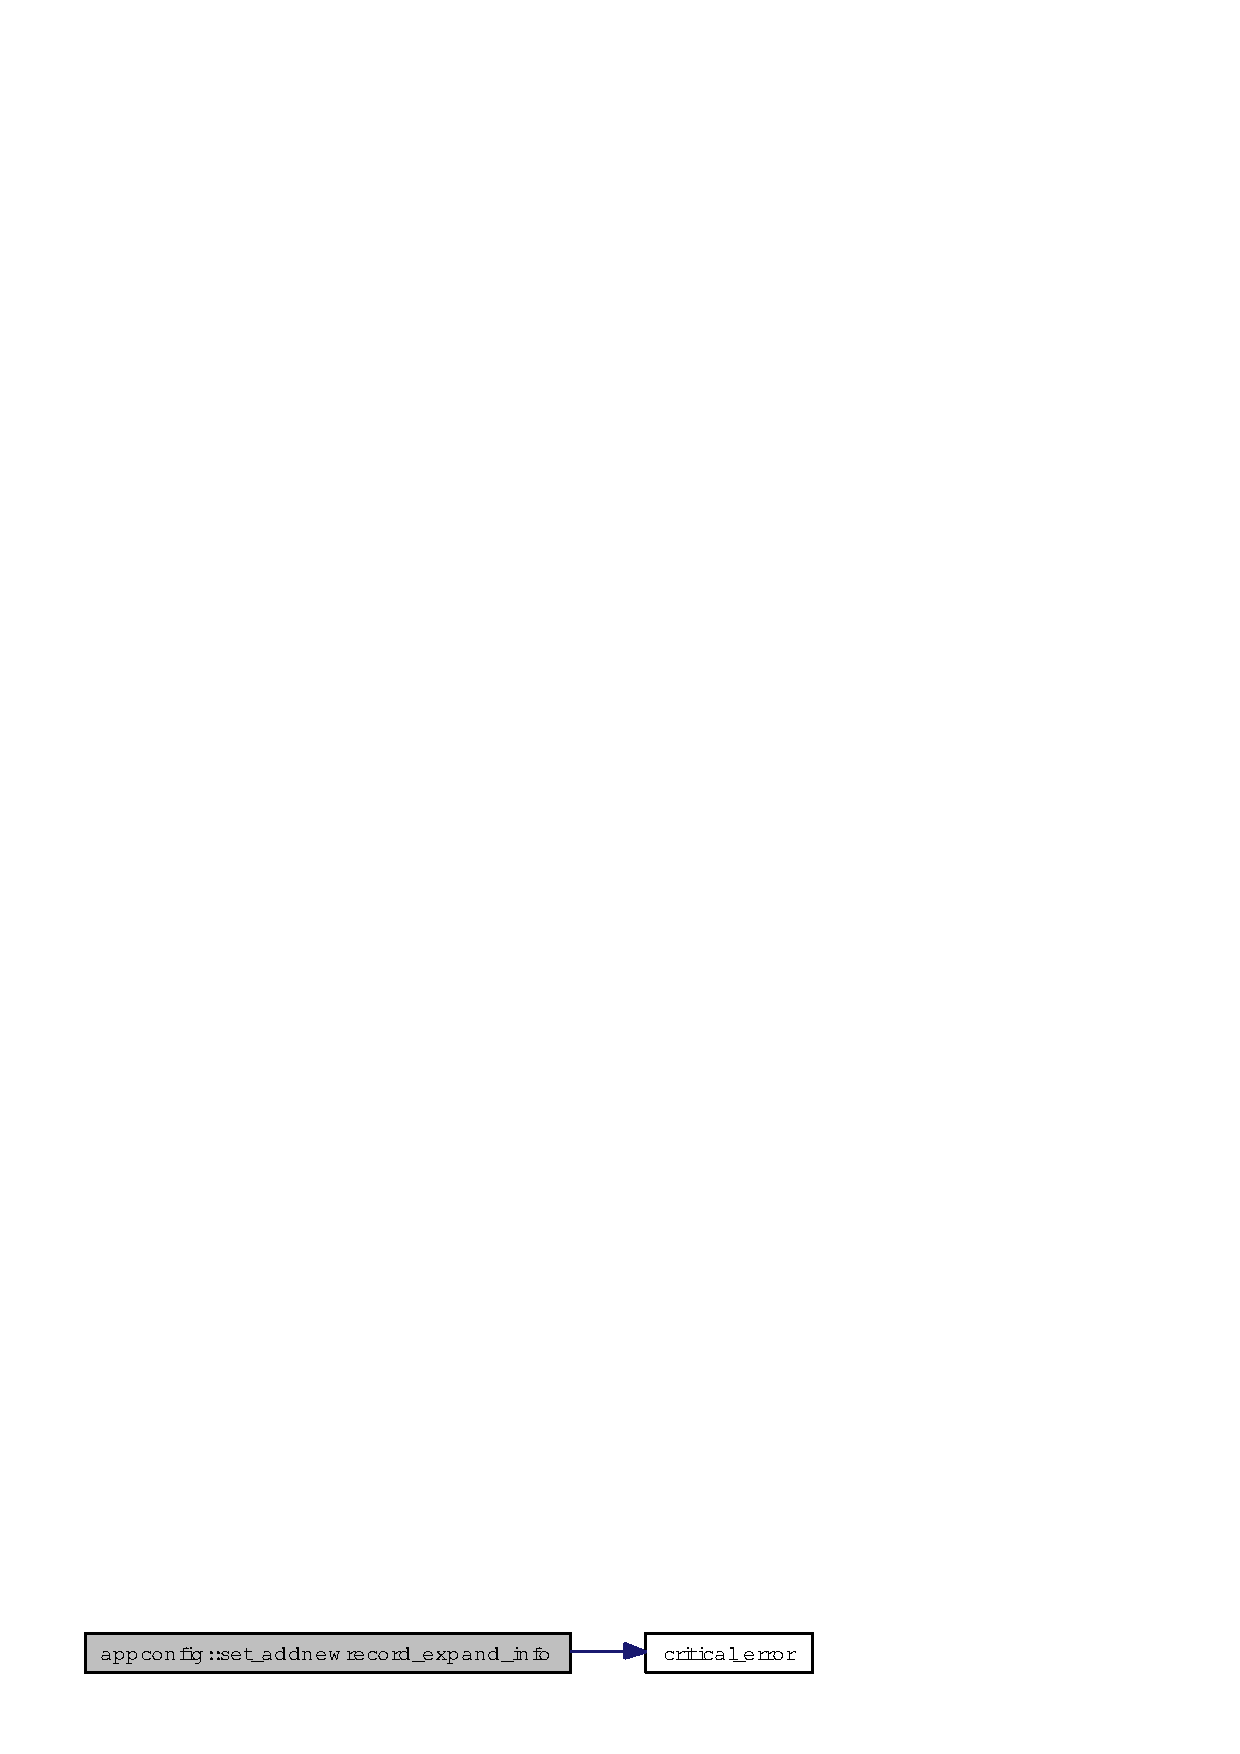
\includegraphics[width=197pt]{classappconfig_380f3e044a57a554dc2d7980a016a3e2_cgraph}
\end{center}
\end{figure}
\index{appconfig@{appconfig}!get_mainwingeometry@{get\_\-mainwingeometry}}
\index{get_mainwingeometry@{get\_\-mainwingeometry}!appconfig@{appconfig}}
\subsubsection{\setlength{\rightskip}{0pt plus 5cm}QRect appconfig::get\_\-mainwingeometry (void)}\label{classappconfig_266005e28aa275a8df212192d9eaaf27}




Definition at line 197 of file appconfig.cpp.

References conf.

Referenced by mainwindow::restore\_\-geometry().

Here is the caller graph for this function:\begin{figure}[H]
\begin{center}
\leavevmode
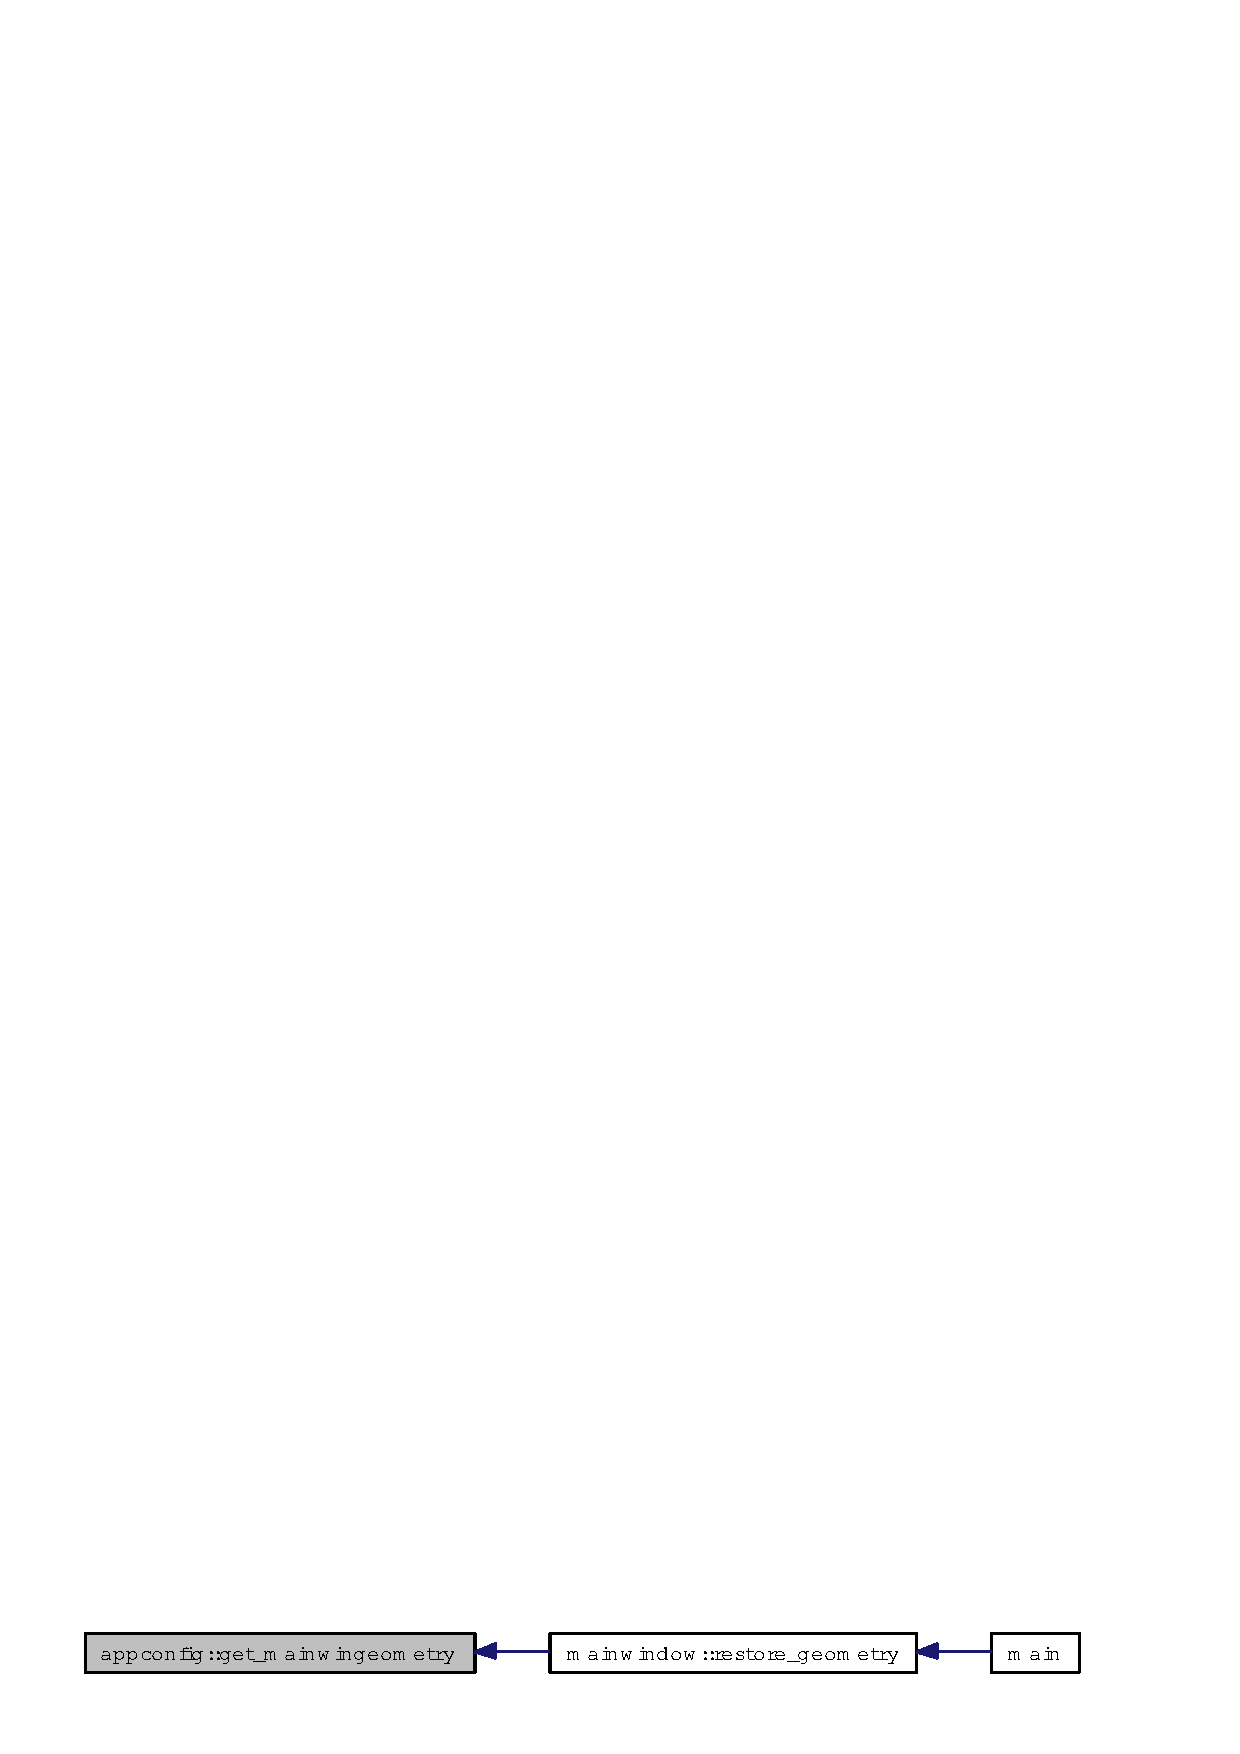
\includegraphics[width=261pt]{classappconfig_266005e28aa275a8df212192d9eaaf27_icgraph}
\end{center}
\end{figure}
\index{appconfig@{appconfig}!set_mainwingeometry@{set\_\-mainwingeometry}}
\index{set_mainwingeometry@{set\_\-mainwingeometry}!appconfig@{appconfig}}
\subsubsection{\setlength{\rightskip}{0pt plus 5cm}void appconfig::set\_\-mainwingeometry (int {\em x}, int {\em y}, int {\em w}, int {\em h})}\label{classappconfig_996f730172676a83dcf58b99f7519cf7}




Definition at line 203 of file appconfig.cpp.

References conf.

Referenced by mainwindow::save\_\-geometry().

Here is the caller graph for this function:\begin{figure}[H]
\begin{center}
\leavevmode
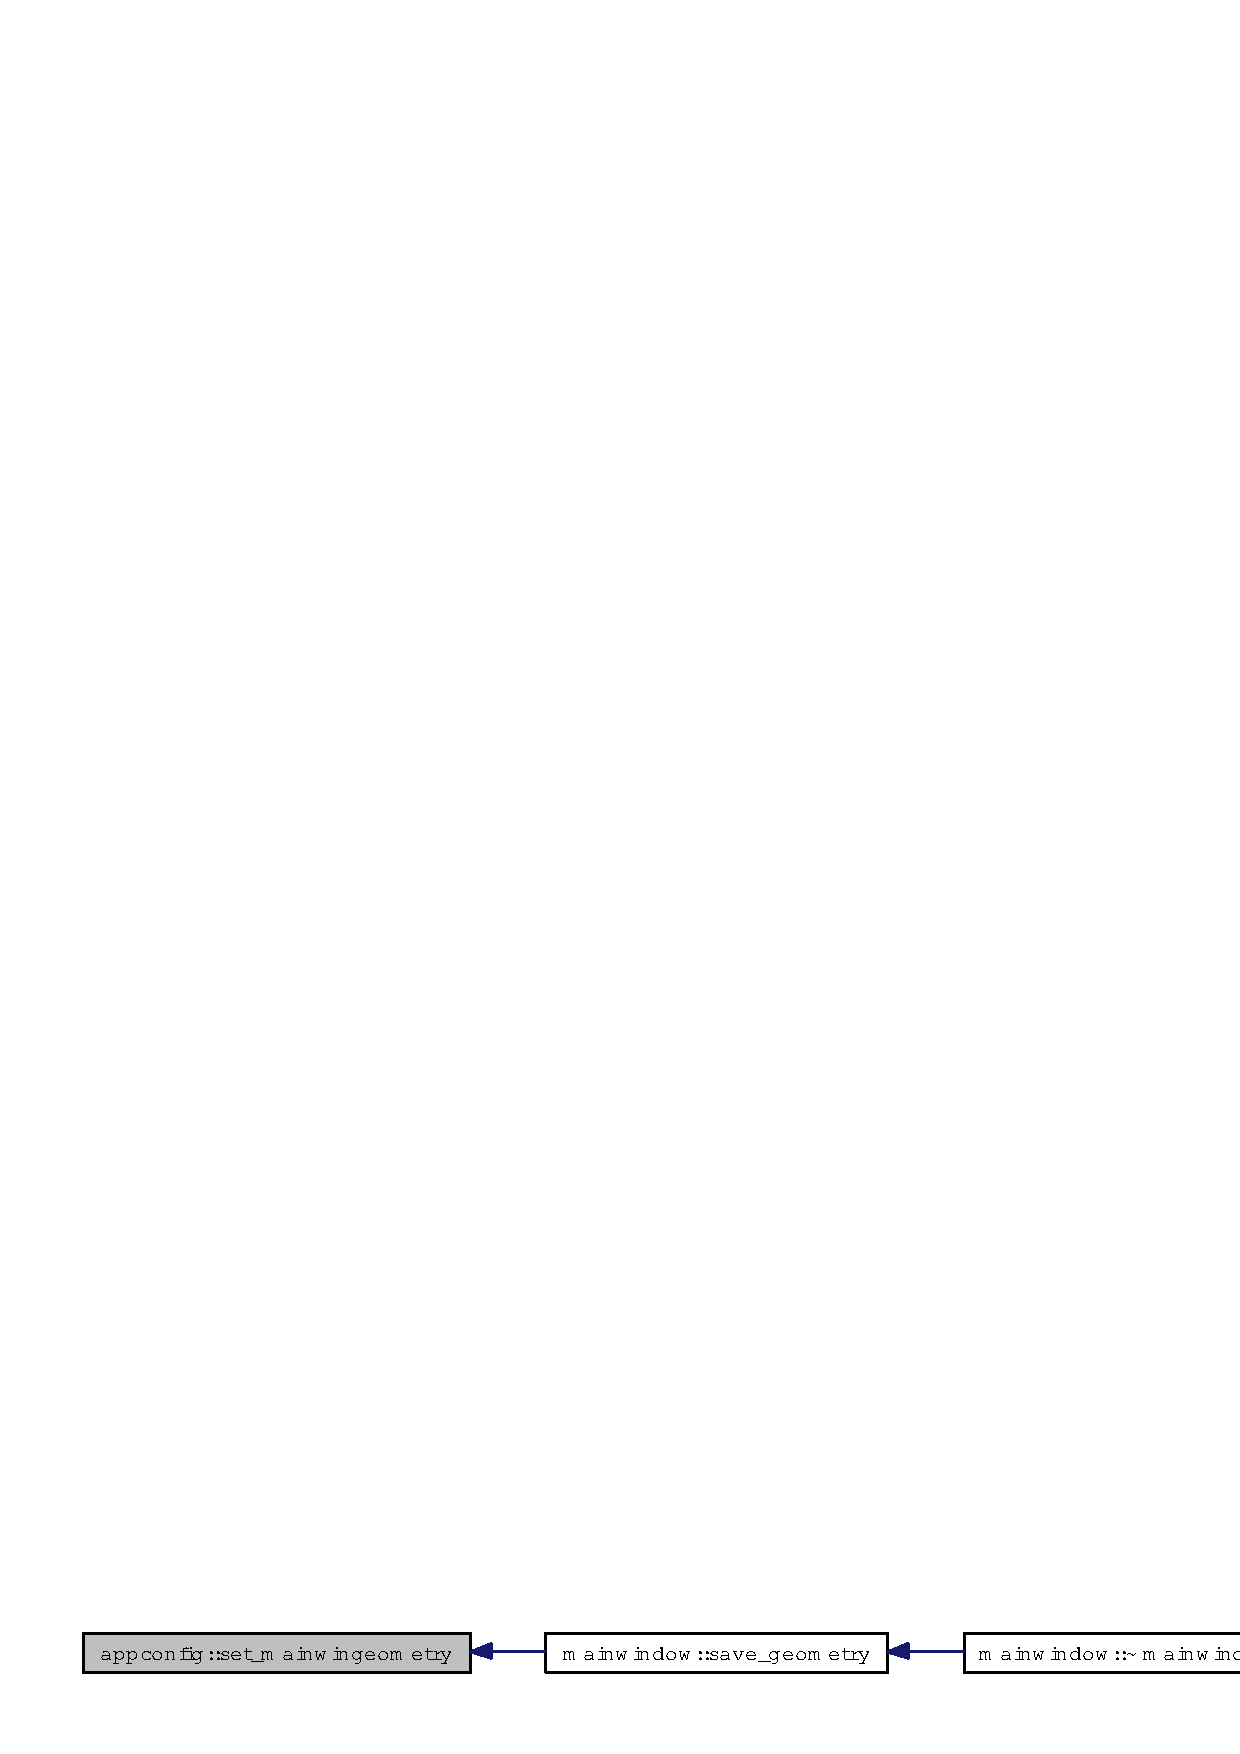
\includegraphics[width=313pt]{classappconfig_996f730172676a83dcf58b99f7519cf7_icgraph}
\end{center}
\end{figure}
\index{appconfig@{appconfig}!get_vspl_size_list@{get\_\-vspl\_\-size\_\-list}}
\index{get_vspl_size_list@{get\_\-vspl\_\-size\_\-list}!appconfig@{appconfig}}
\subsubsection{\setlength{\rightskip}{0pt plus 5cm}QList$<$ int $>$ appconfig::get\_\-vspl\_\-size\_\-list (void)}\label{classappconfig_578b013308a692c38f1c99530b8dbdd1}




Definition at line 210 of file appconfig.cpp.

References get\_\-splitter\_\-size\_\-list().

Referenced by mainwindow::restore\_\-geometry().

Here is the call graph for this function:\begin{figure}[H]
\begin{center}
\leavevmode
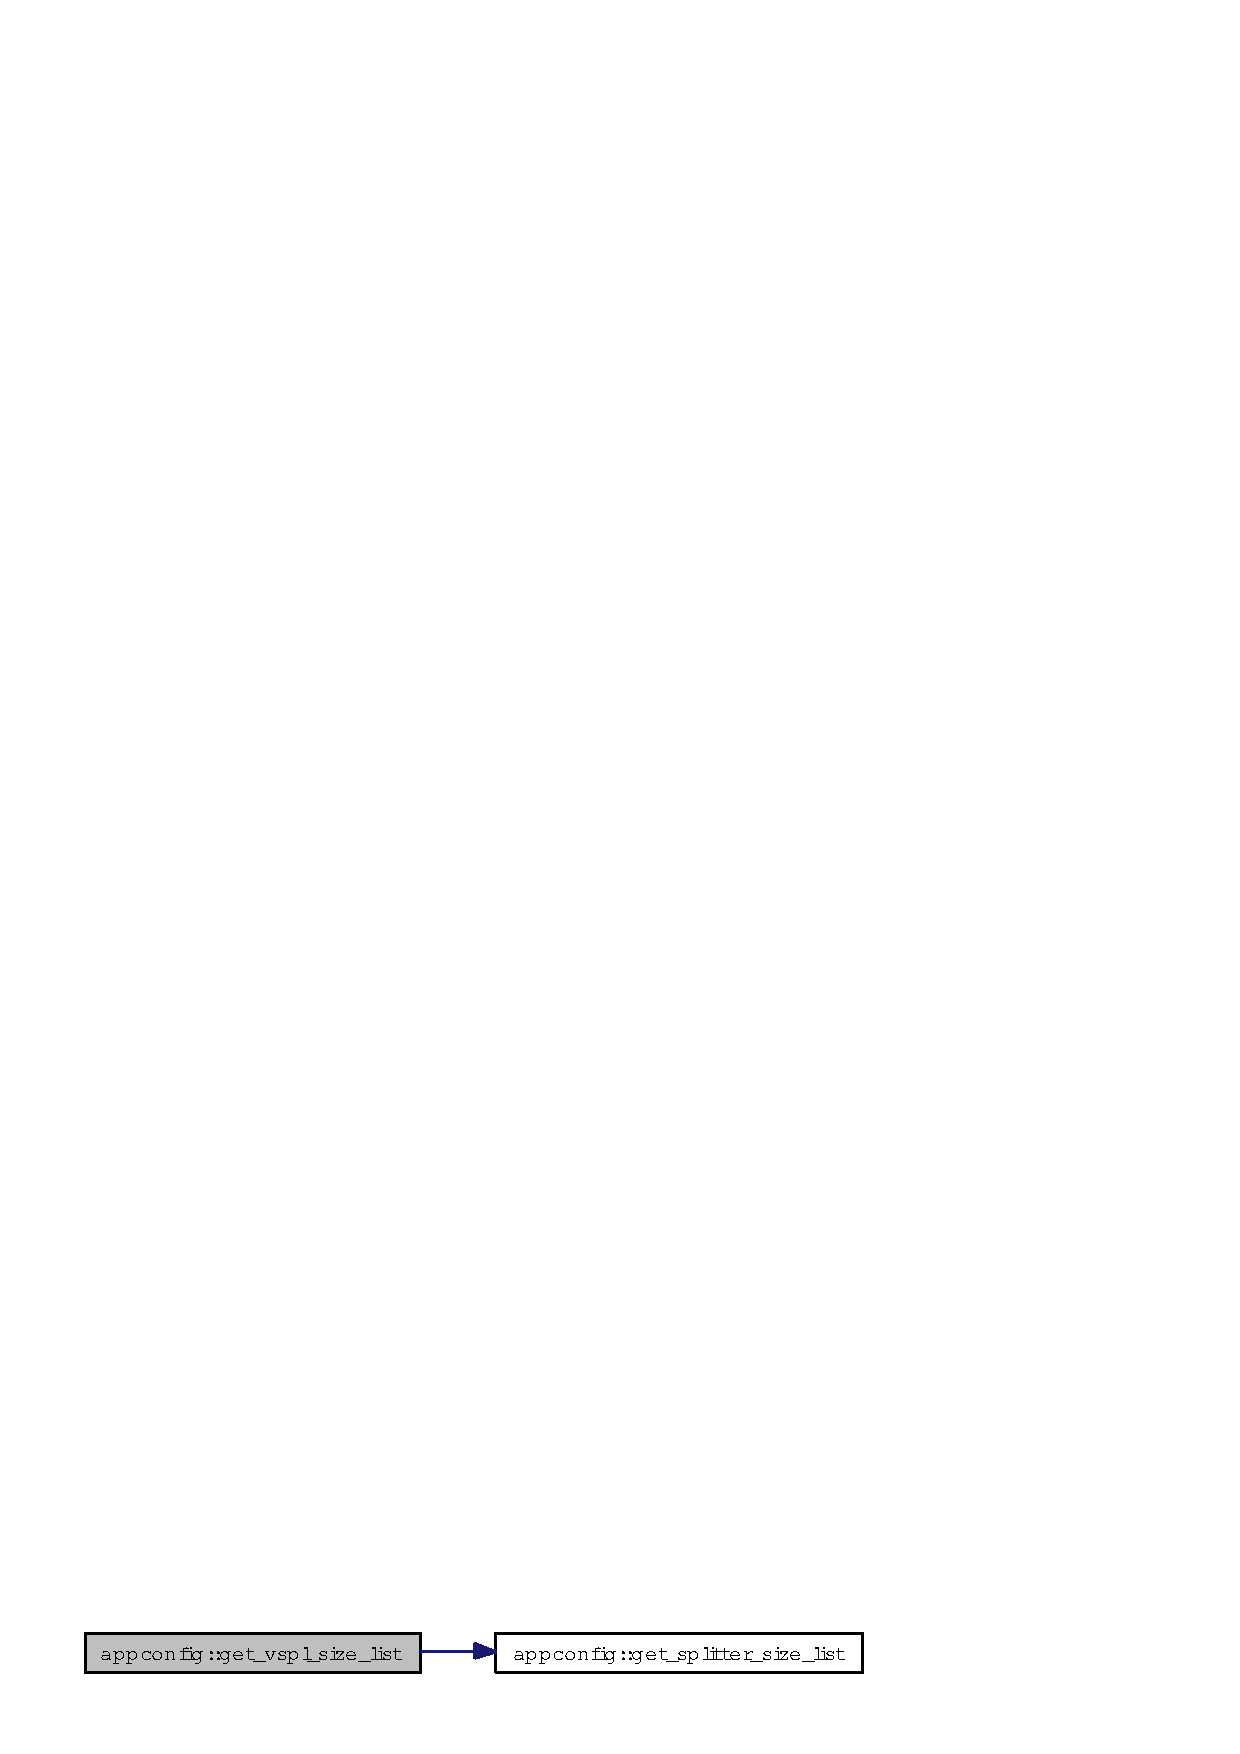
\includegraphics[width=209pt]{classappconfig_578b013308a692c38f1c99530b8dbdd1_cgraph}
\end{center}
\end{figure}


Here is the caller graph for this function:\begin{figure}[H]
\begin{center}
\leavevmode
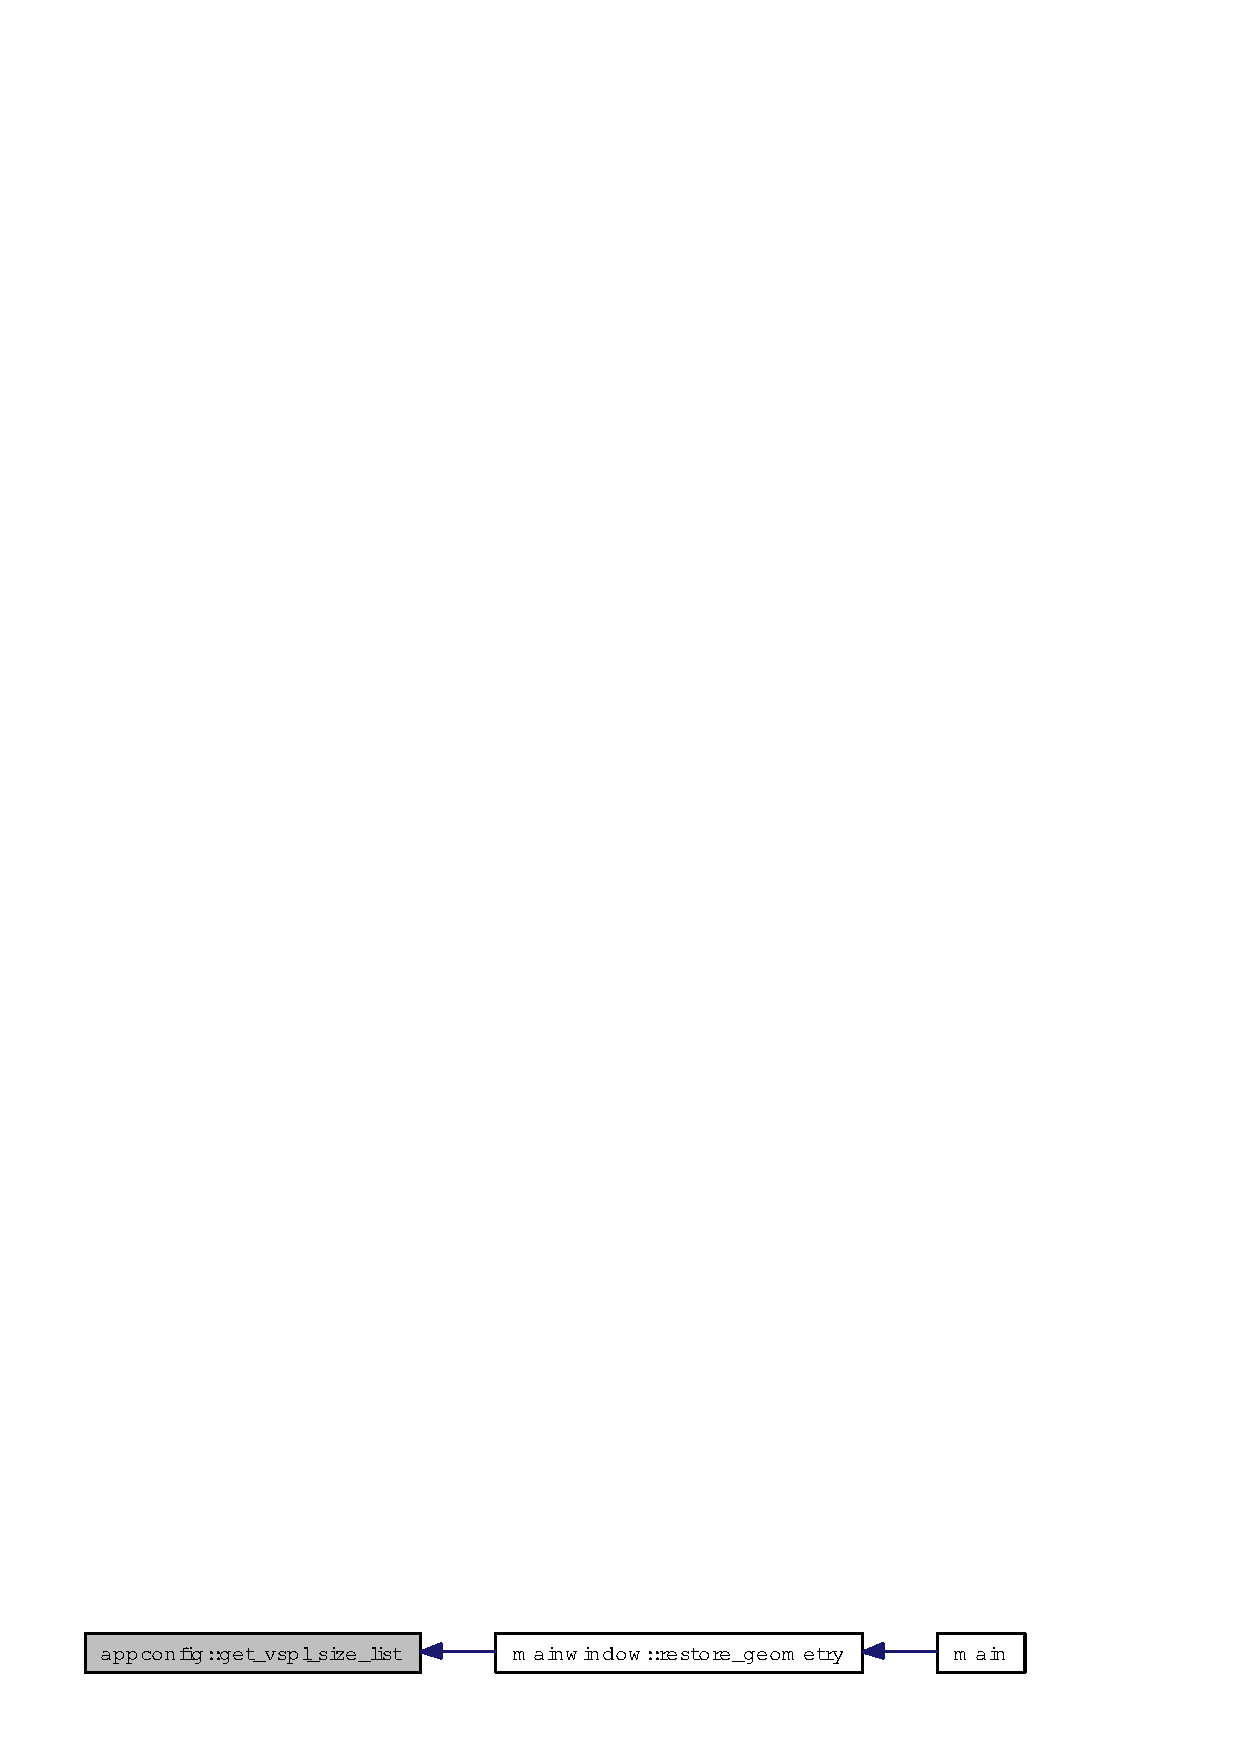
\includegraphics[width=248pt]{classappconfig_578b013308a692c38f1c99530b8dbdd1_icgraph}
\end{center}
\end{figure}
\index{appconfig@{appconfig}!set_vspl_size_list@{set\_\-vspl\_\-size\_\-list}}
\index{set_vspl_size_list@{set\_\-vspl\_\-size\_\-list}!appconfig@{appconfig}}
\subsubsection{\setlength{\rightskip}{0pt plus 5cm}void appconfig::set\_\-vspl\_\-size\_\-list (QList$<$ int $>$ {\em list})}\label{classappconfig_648e45ffc122e3e4fb1bfc998b82e250}




Definition at line 216 of file appconfig.cpp.

References set\_\-splitter\_\-size\_\-list().

Referenced by mainwindow::save\_\-geometry().

Here is the call graph for this function:\begin{figure}[H]
\begin{center}
\leavevmode
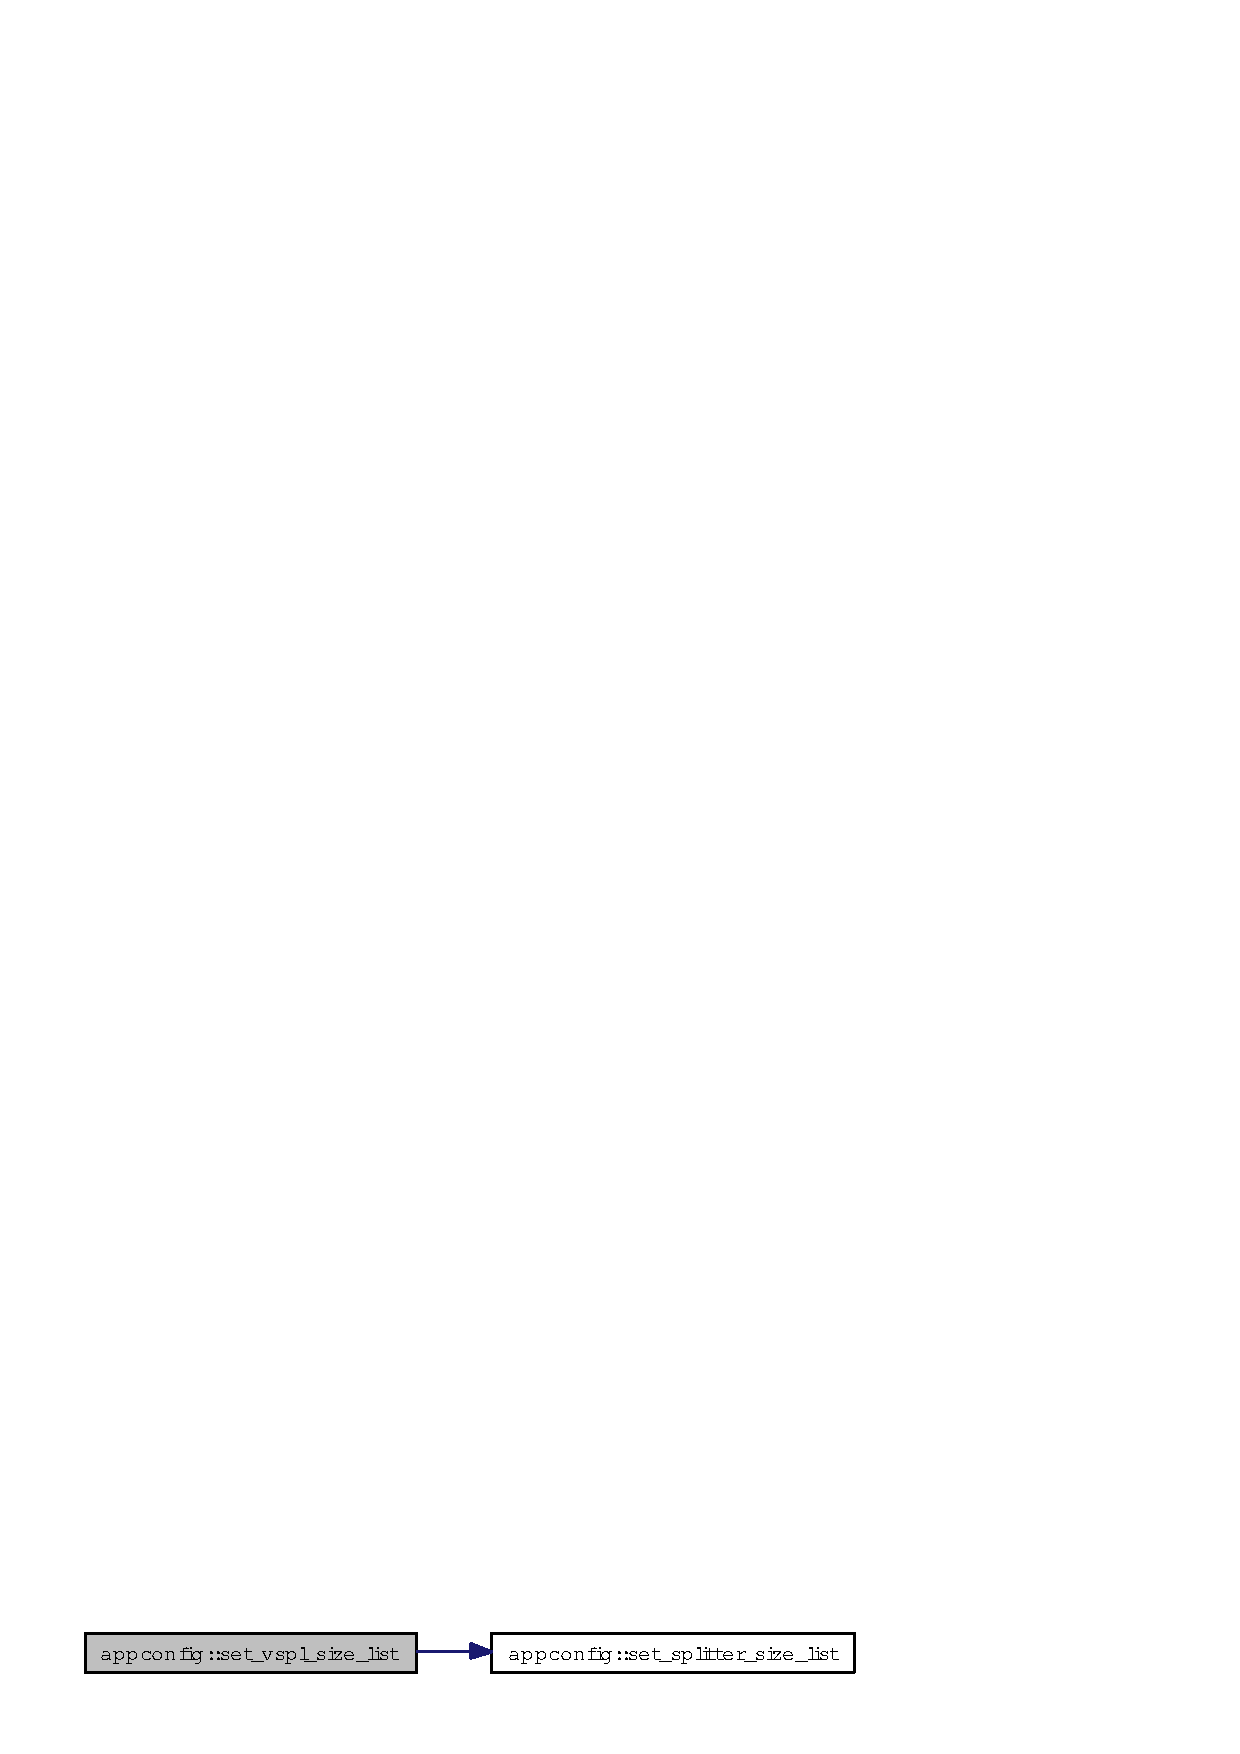
\includegraphics[width=207pt]{classappconfig_648e45ffc122e3e4fb1bfc998b82e250_cgraph}
\end{center}
\end{figure}


Here is the caller graph for this function:\begin{figure}[H]
\begin{center}
\leavevmode
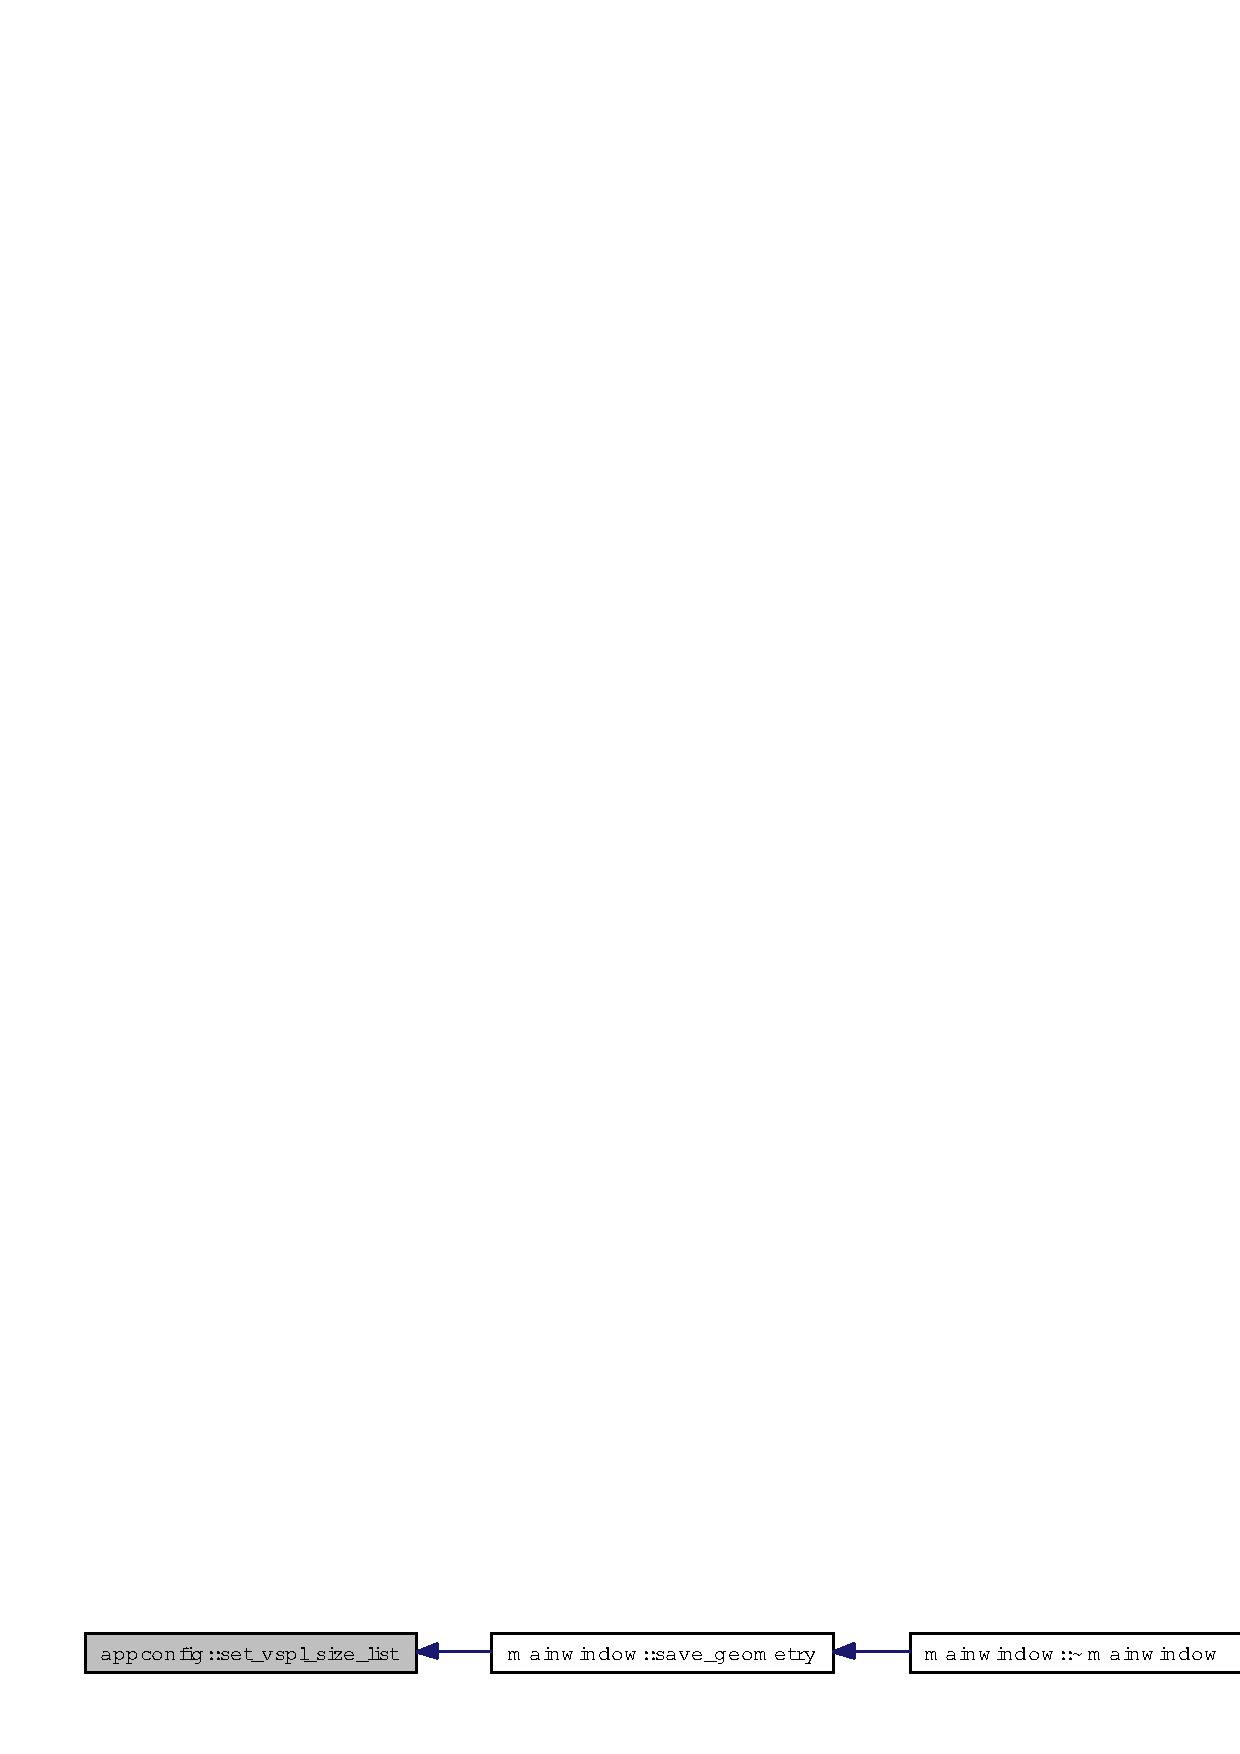
\includegraphics[width=300pt]{classappconfig_648e45ffc122e3e4fb1bfc998b82e250_icgraph}
\end{center}
\end{figure}
\index{appconfig@{appconfig}!get_hspl_size_list@{get\_\-hspl\_\-size\_\-list}}
\index{get_hspl_size_list@{get\_\-hspl\_\-size\_\-list}!appconfig@{appconfig}}
\subsubsection{\setlength{\rightskip}{0pt plus 5cm}QList$<$ int $>$ appconfig::get\_\-hspl\_\-size\_\-list (void)}\label{classappconfig_9606e4902b9739393279276ada9b0967}




Definition at line 222 of file appconfig.cpp.

References get\_\-splitter\_\-size\_\-list().

Referenced by mainwindow::restore\_\-geometry().

Here is the call graph for this function:\begin{figure}[H]
\begin{center}
\leavevmode
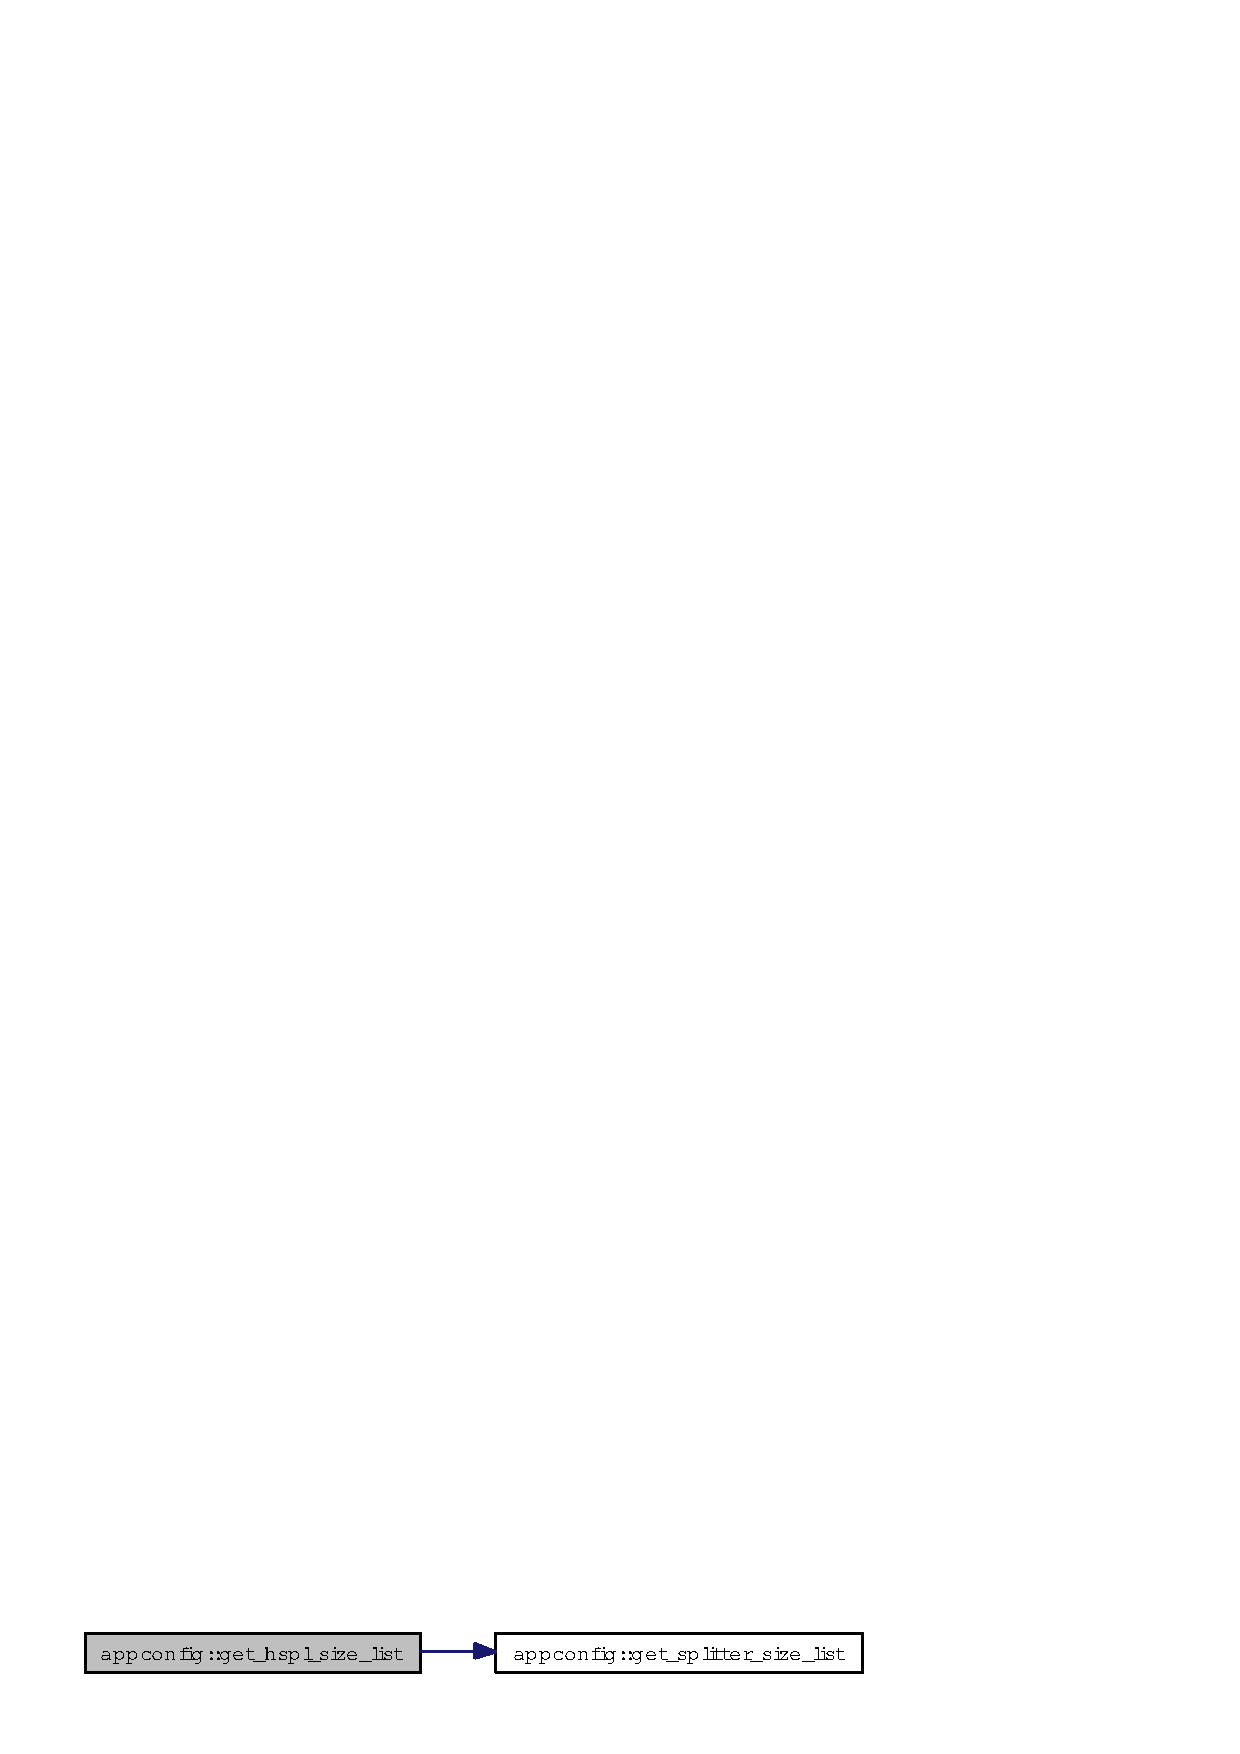
\includegraphics[width=209pt]{classappconfig_9606e4902b9739393279276ada9b0967_cgraph}
\end{center}
\end{figure}


Here is the caller graph for this function:\begin{figure}[H]
\begin{center}
\leavevmode
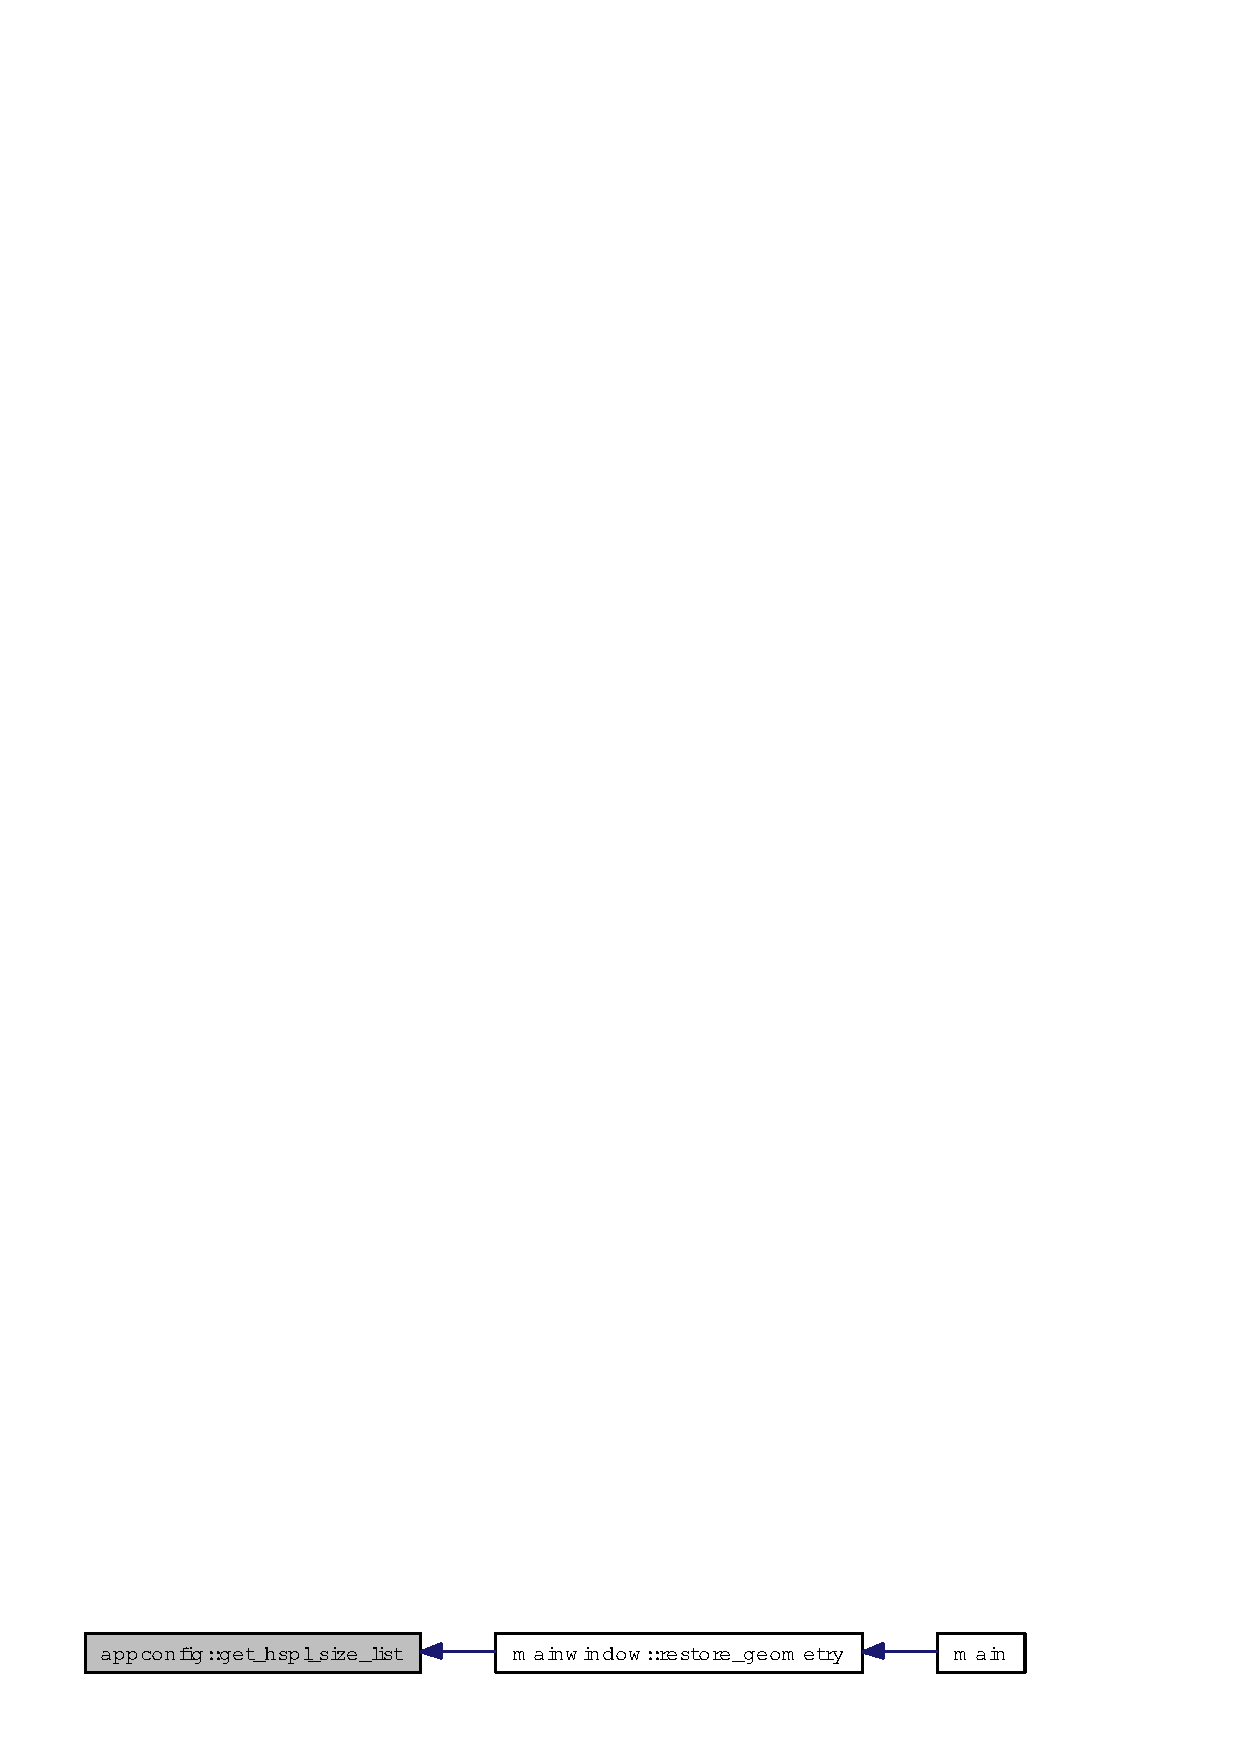
\includegraphics[width=248pt]{classappconfig_9606e4902b9739393279276ada9b0967_icgraph}
\end{center}
\end{figure}
\index{appconfig@{appconfig}!set_hspl_size_list@{set\_\-hspl\_\-size\_\-list}}
\index{set_hspl_size_list@{set\_\-hspl\_\-size\_\-list}!appconfig@{appconfig}}
\subsubsection{\setlength{\rightskip}{0pt plus 5cm}void appconfig::set\_\-hspl\_\-size\_\-list (QList$<$ int $>$ {\em list})}\label{classappconfig_321f62af83196d0409ab5f2f1197de83}




Definition at line 228 of file appconfig.cpp.

References set\_\-splitter\_\-size\_\-list().

Referenced by mainwindow::save\_\-geometry().

Here is the call graph for this function:\begin{figure}[H]
\begin{center}
\leavevmode
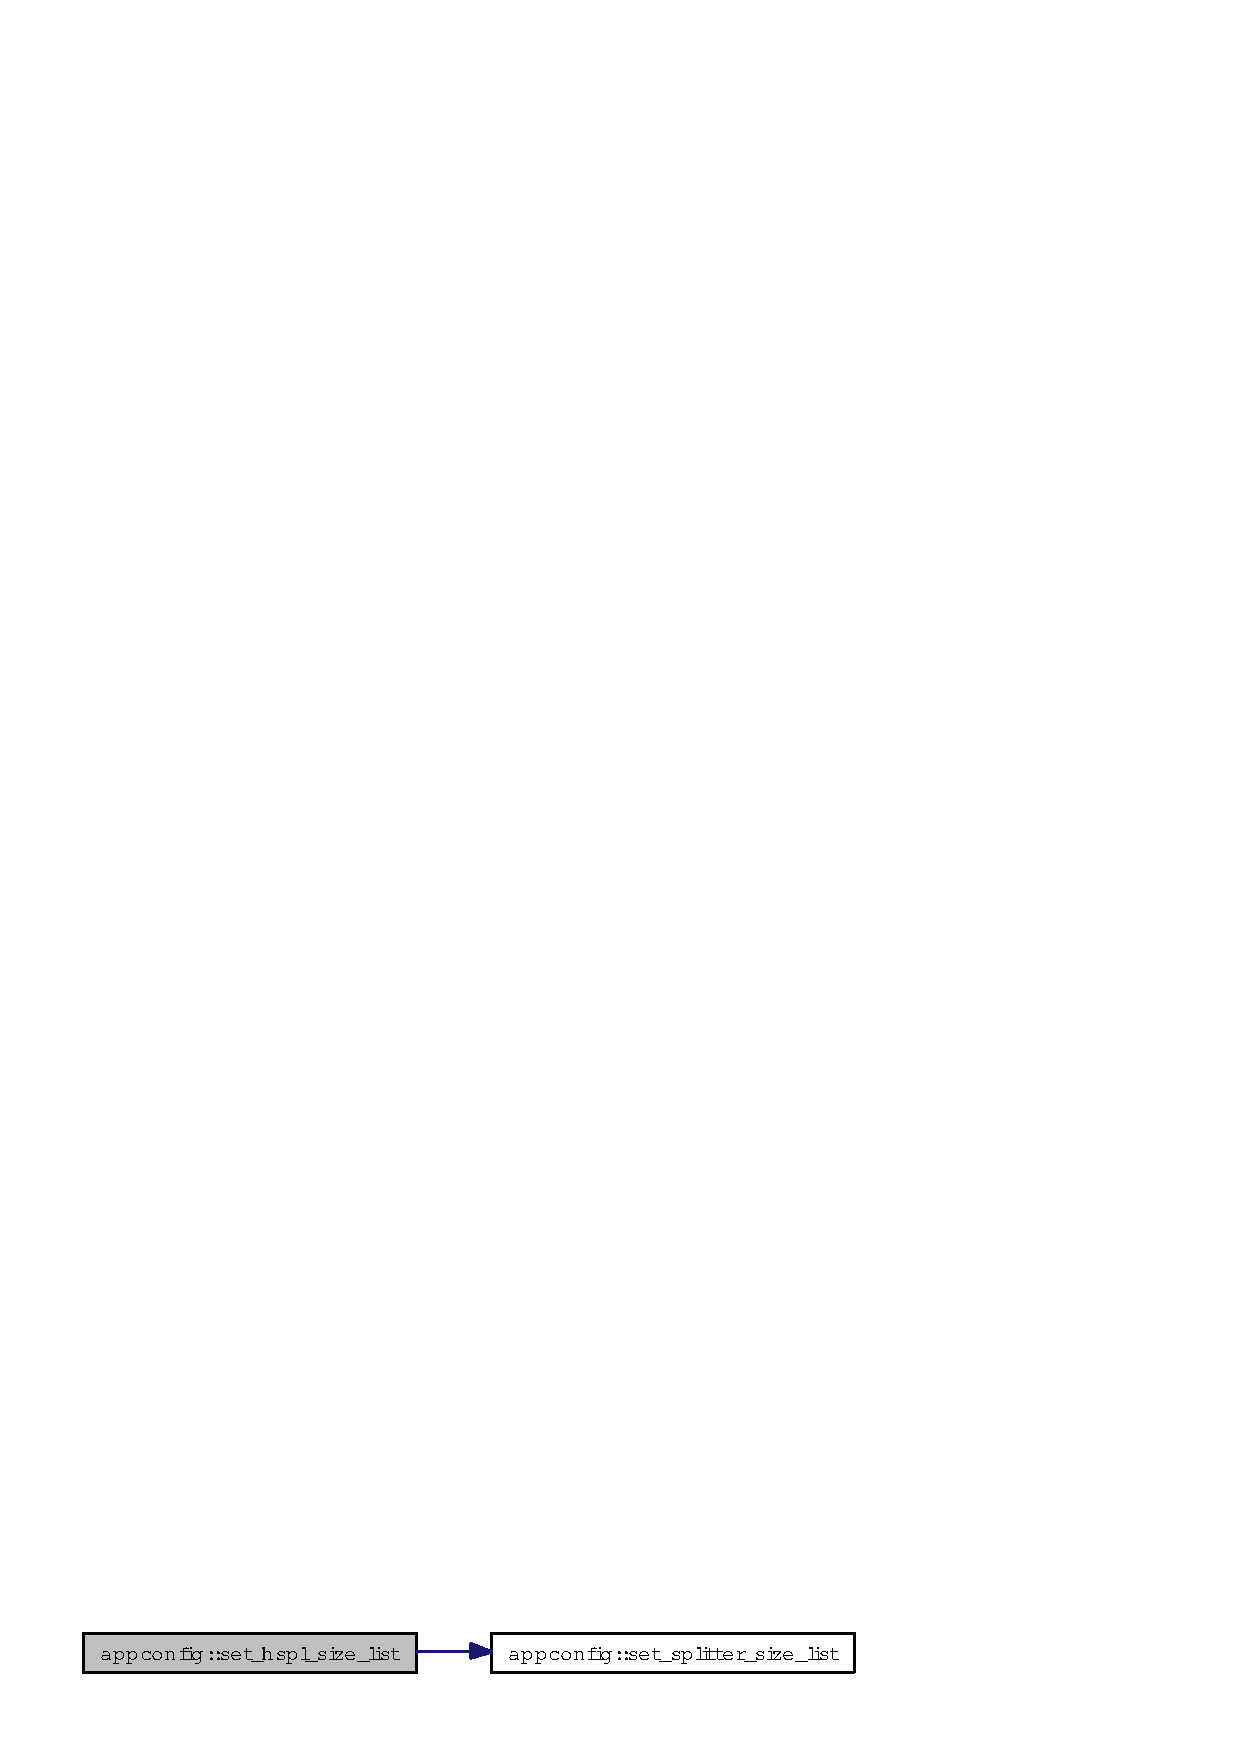
\includegraphics[width=207pt]{classappconfig_321f62af83196d0409ab5f2f1197de83_cgraph}
\end{center}
\end{figure}


Here is the caller graph for this function:\begin{figure}[H]
\begin{center}
\leavevmode
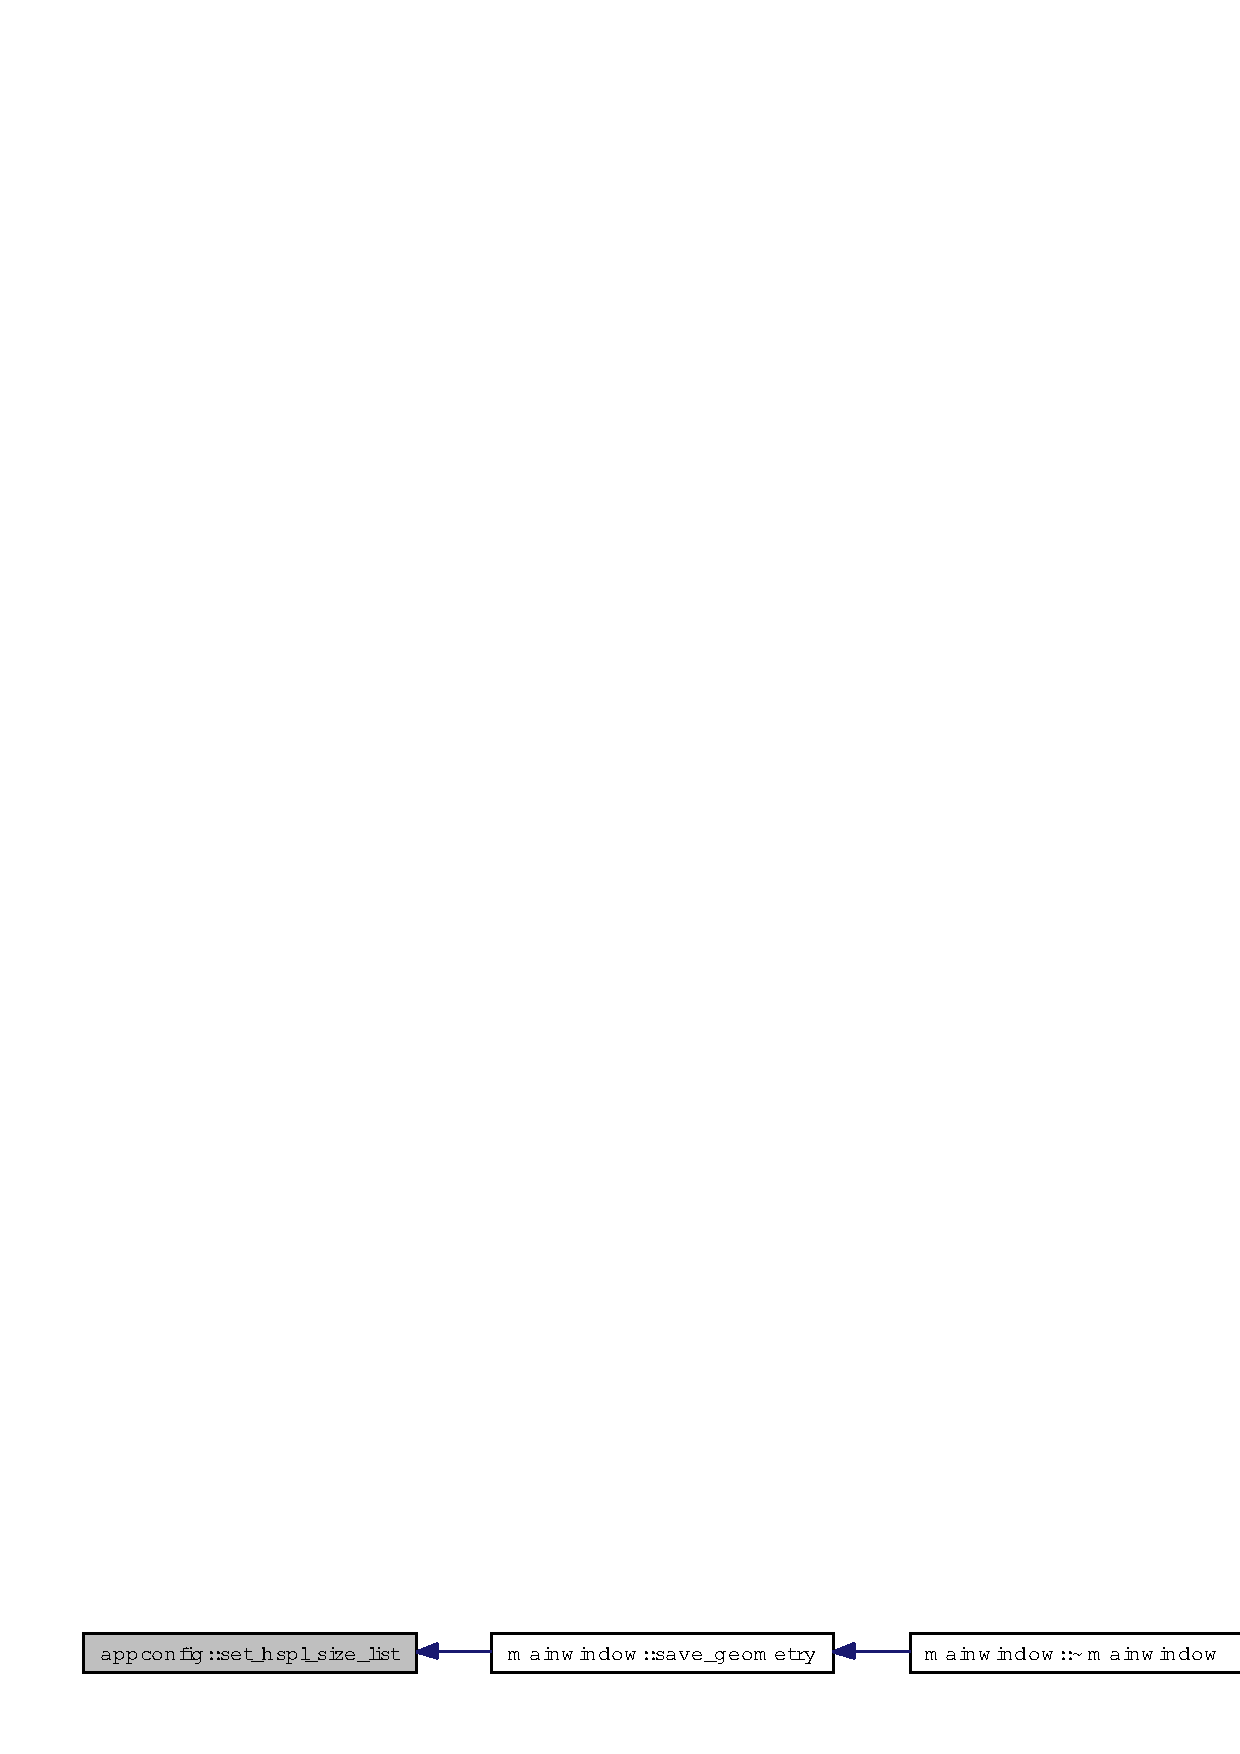
\includegraphics[width=300pt]{classappconfig_321f62af83196d0409ab5f2f1197de83_icgraph}
\end{center}
\end{figure}
\index{appconfig@{appconfig}!get_findsplitter_size_list@{get\_\-findsplitter\_\-size\_\-list}}
\index{get_findsplitter_size_list@{get\_\-findsplitter\_\-size\_\-list}!appconfig@{appconfig}}
\subsubsection{\setlength{\rightskip}{0pt plus 5cm}QList$<$ int $>$ appconfig::get\_\-findsplitter\_\-size\_\-list (void)}\label{classappconfig_7ff8392b05f0a5a068a13efbc829e30e}




Definition at line 234 of file appconfig.cpp.

References get\_\-splitter\_\-size\_\-list().

Referenced by mainwindow::restore\_\-geometry().

Here is the call graph for this function:\begin{figure}[H]
\begin{center}
\leavevmode
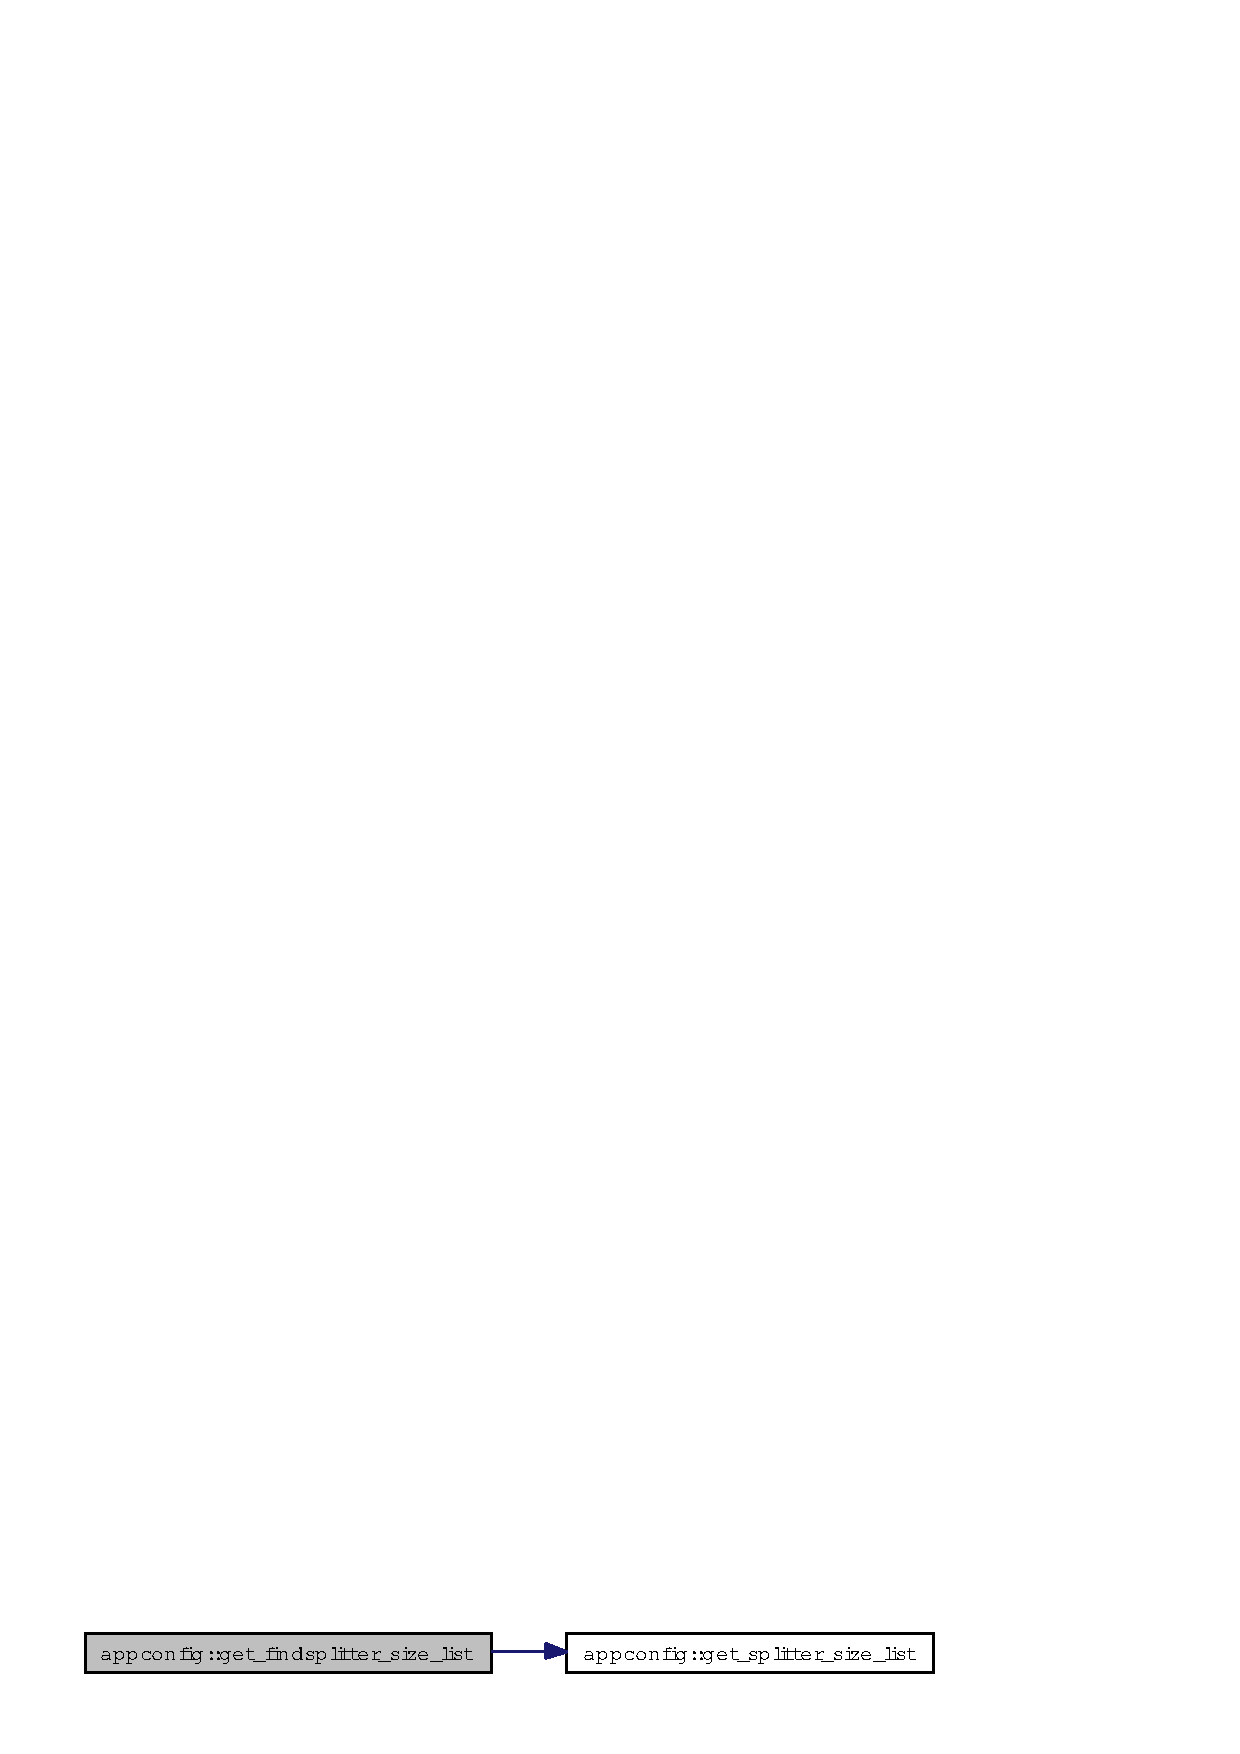
\includegraphics[width=226pt]{classappconfig_7ff8392b05f0a5a068a13efbc829e30e_cgraph}
\end{center}
\end{figure}


Here is the caller graph for this function:\begin{figure}[H]
\begin{center}
\leavevmode
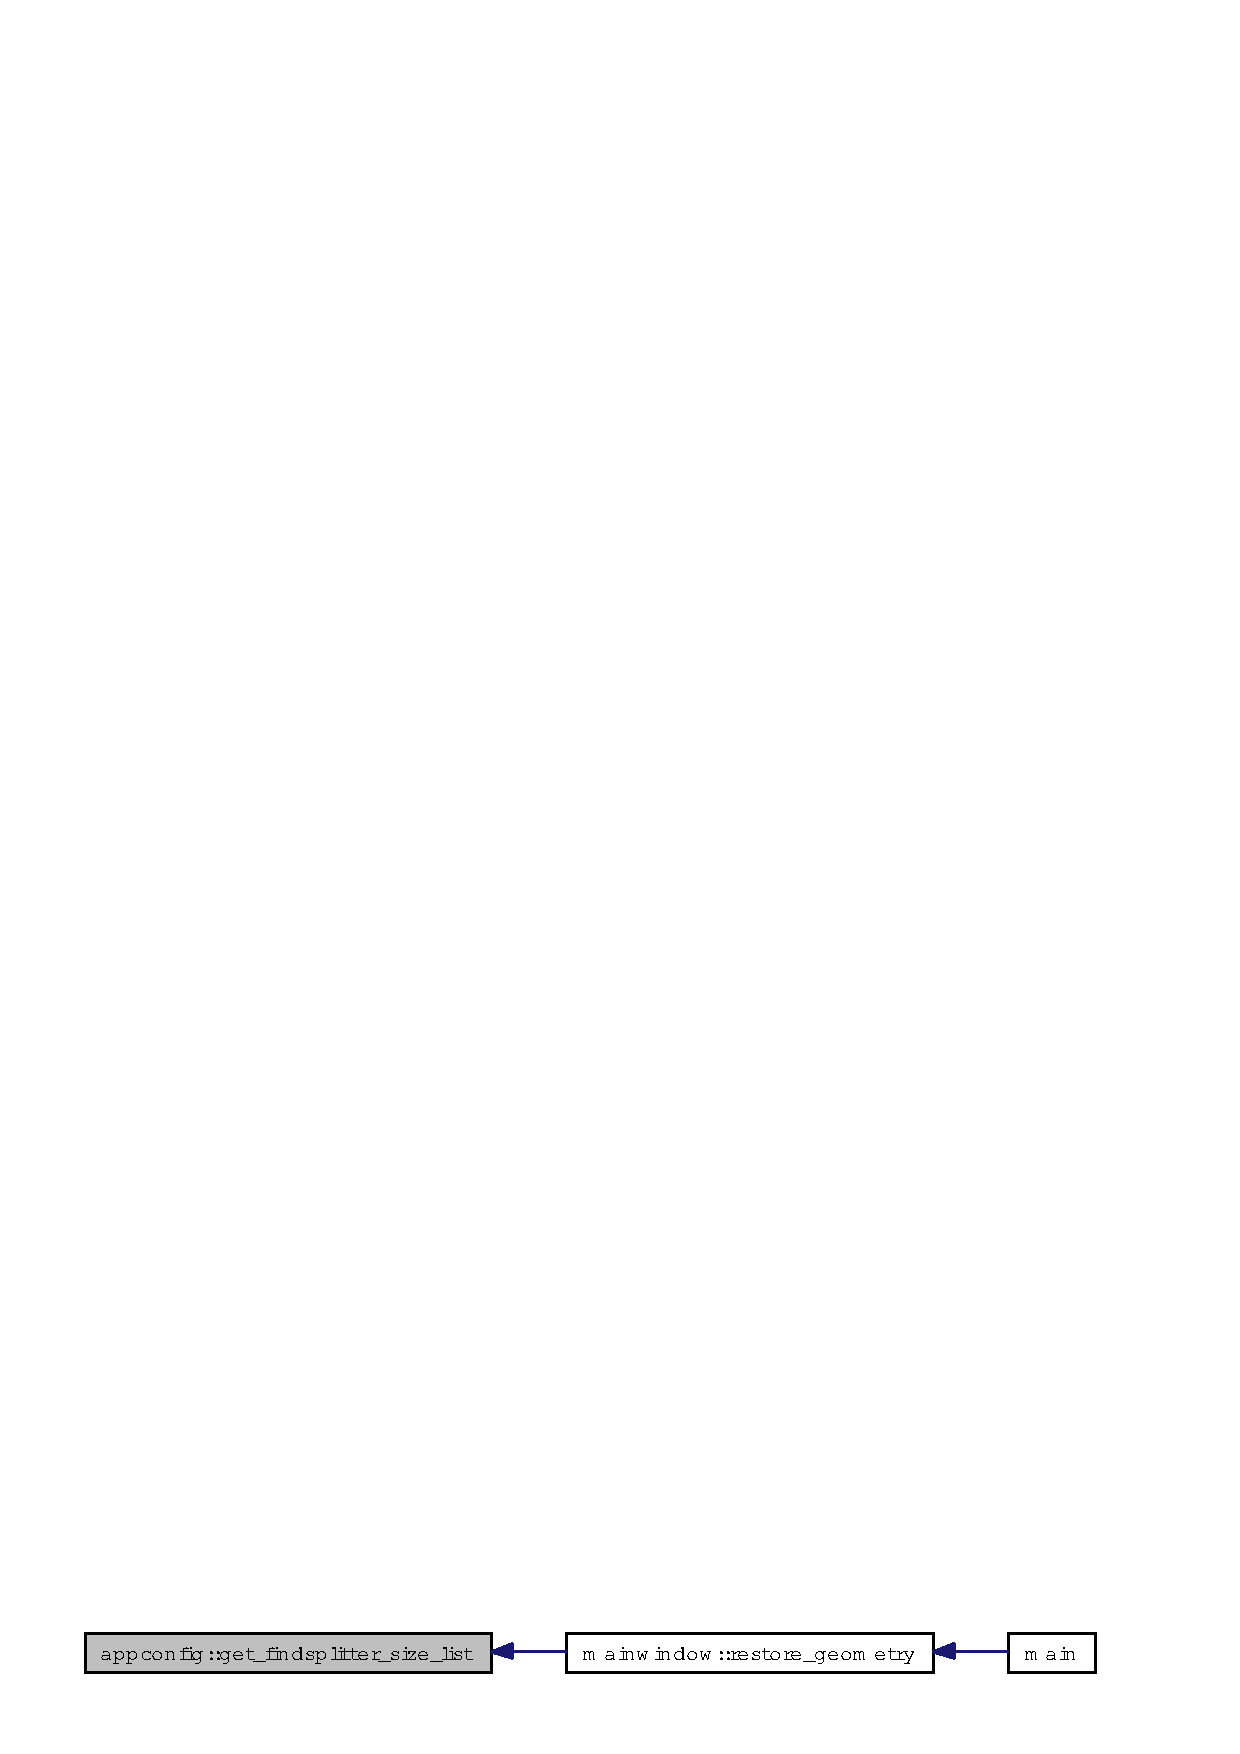
\includegraphics[width=265pt]{classappconfig_7ff8392b05f0a5a068a13efbc829e30e_icgraph}
\end{center}
\end{figure}
\index{appconfig@{appconfig}!set_findsplitter_size_list@{set\_\-findsplitter\_\-size\_\-list}}
\index{set_findsplitter_size_list@{set\_\-findsplitter\_\-size\_\-list}!appconfig@{appconfig}}
\subsubsection{\setlength{\rightskip}{0pt plus 5cm}void appconfig::set\_\-findsplitter\_\-size\_\-list (QList$<$ int $>$ {\em list})}\label{classappconfig_3d381a23dd11f7c1eaa9516ba2a069da}




Definition at line 240 of file appconfig.cpp.

References set\_\-splitter\_\-size\_\-list().

Referenced by mainwindow::save\_\-geometry(), and findscreen::widget\_\-hide().

Here is the call graph for this function:\begin{figure}[H]
\begin{center}
\leavevmode
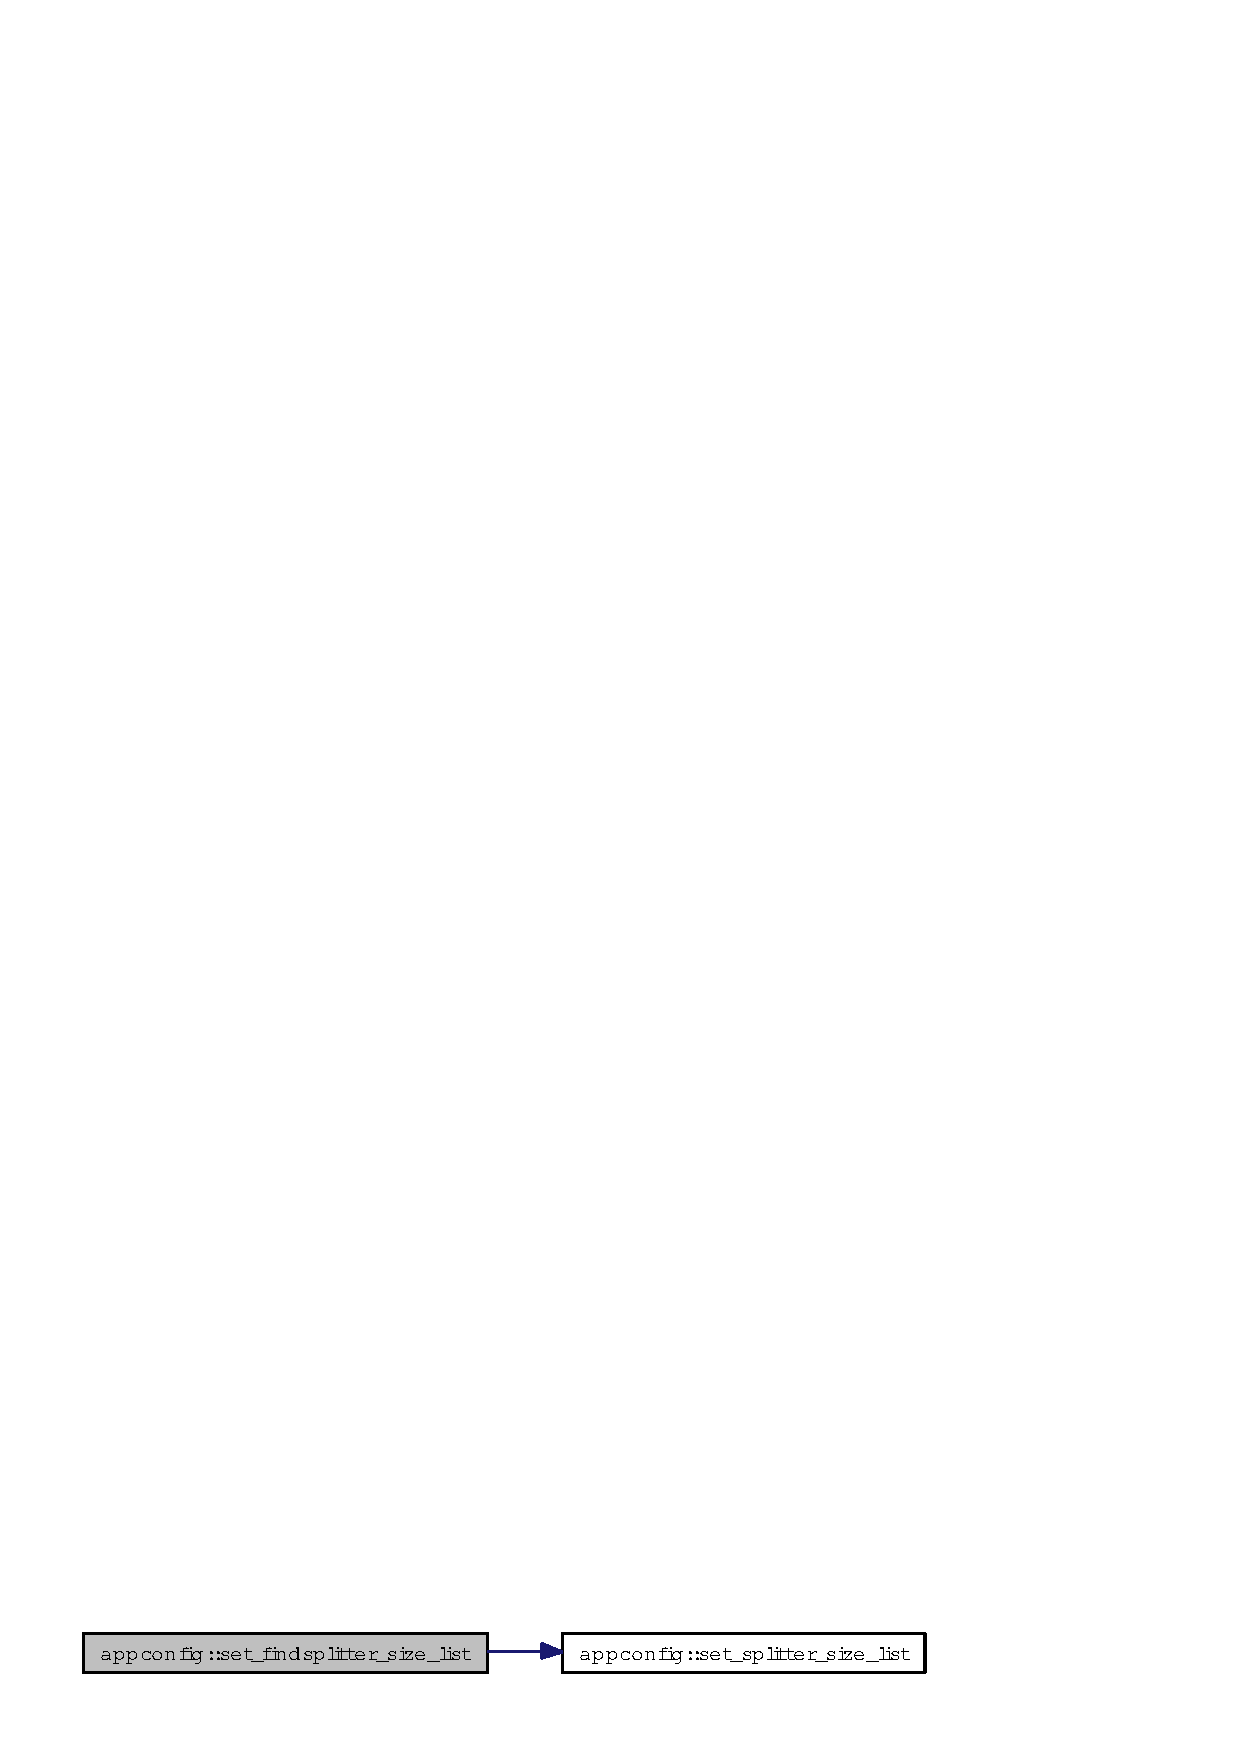
\includegraphics[width=224pt]{classappconfig_3d381a23dd11f7c1eaa9516ba2a069da_cgraph}
\end{center}
\end{figure}


Here is the caller graph for this function:\begin{figure}[H]
\begin{center}
\leavevmode
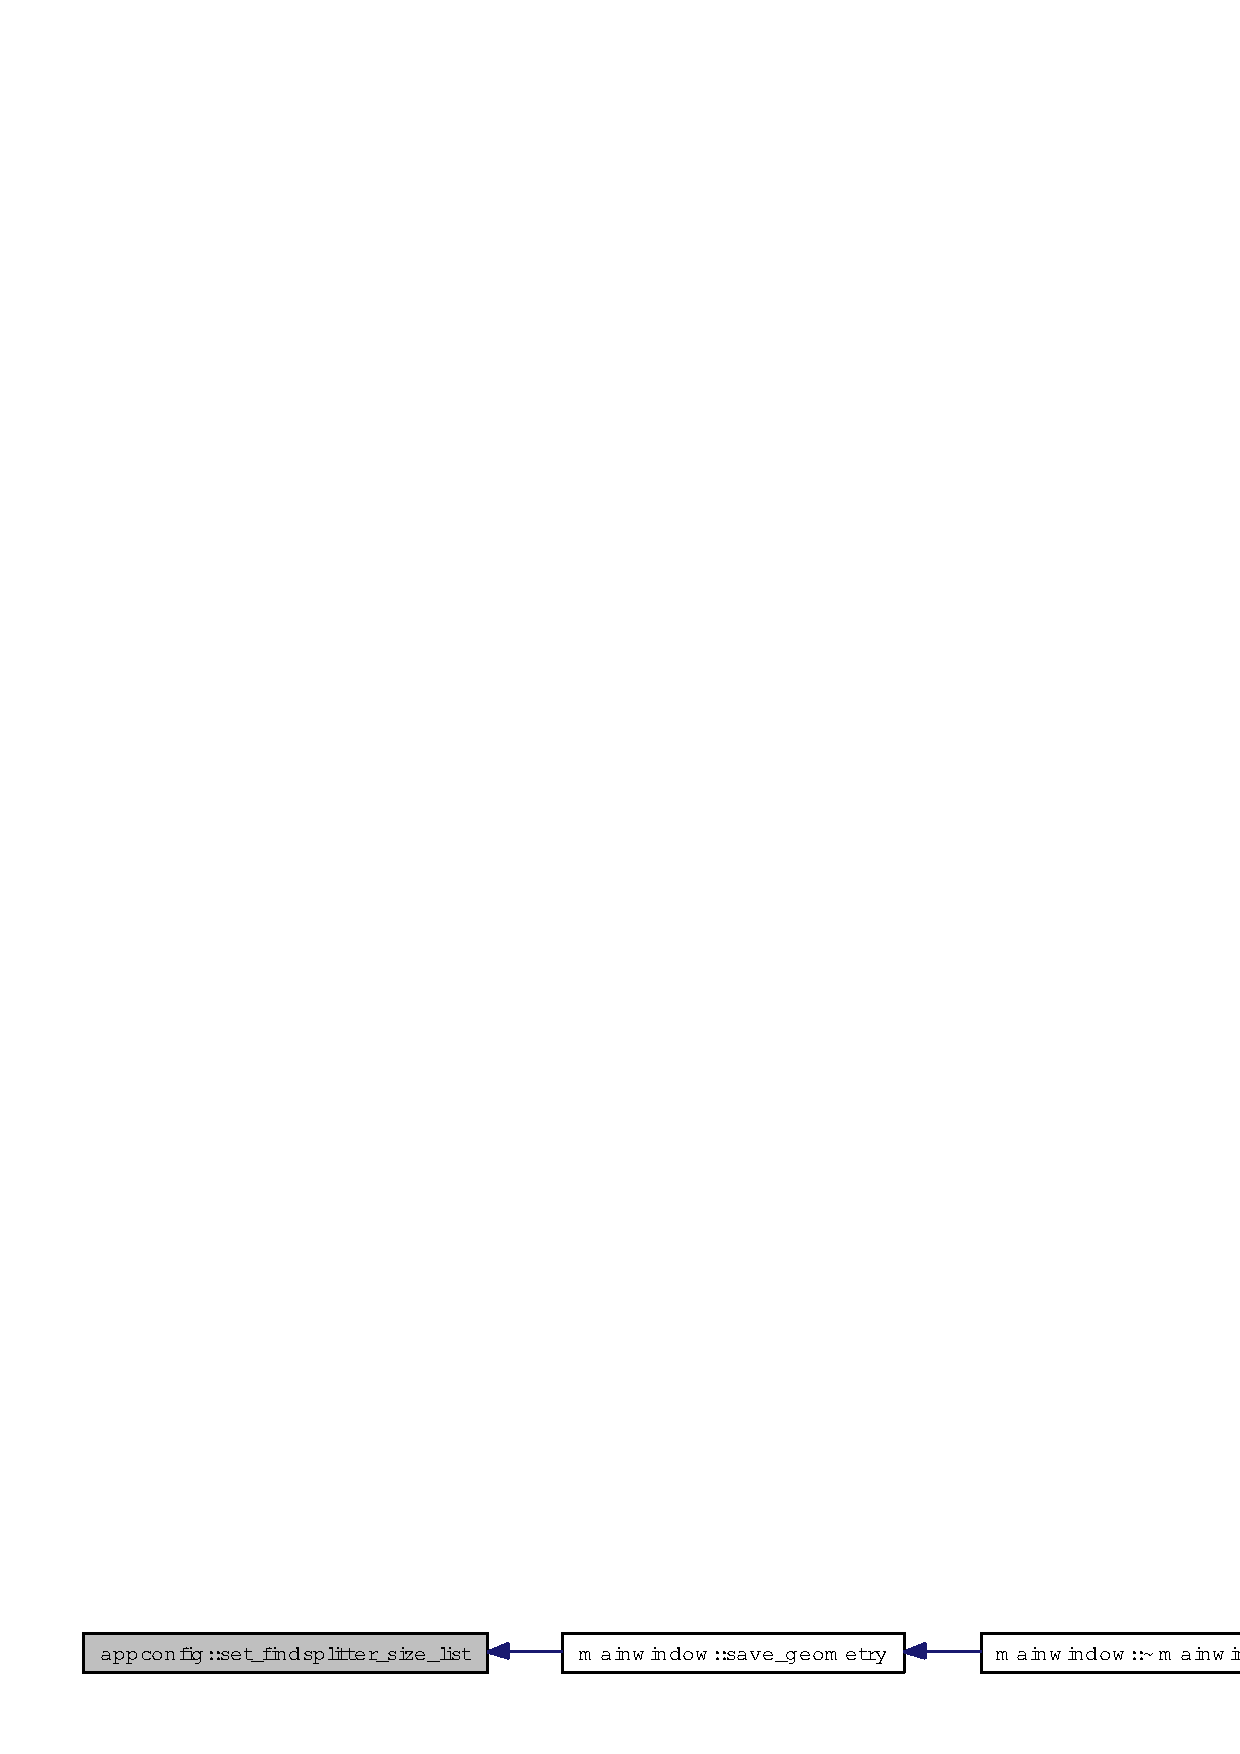
\includegraphics[width=317pt]{classappconfig_3d381a23dd11f7c1eaa9516ba2a069da_icgraph}
\end{center}
\end{figure}
\index{appconfig@{appconfig}!get_splitter_size_list@{get\_\-splitter\_\-size\_\-list}}
\index{get_splitter_size_list@{get\_\-splitter\_\-size\_\-list}!appconfig@{appconfig}}
\subsubsection{\setlength{\rightskip}{0pt plus 5cm}QList$<$ int $>$ appconfig::get\_\-splitter\_\-size\_\-list (QString {\em name})}\label{classappconfig_2e35d75471242db7840adf8058c861d4}




Definition at line 246 of file appconfig.cpp.

References conf.

Referenced by get\_\-findsplitter\_\-size\_\-list(), get\_\-hspl\_\-size\_\-list(), and get\_\-vspl\_\-size\_\-list().

Here is the caller graph for this function:\begin{figure}[H]
\begin{center}
\leavevmode
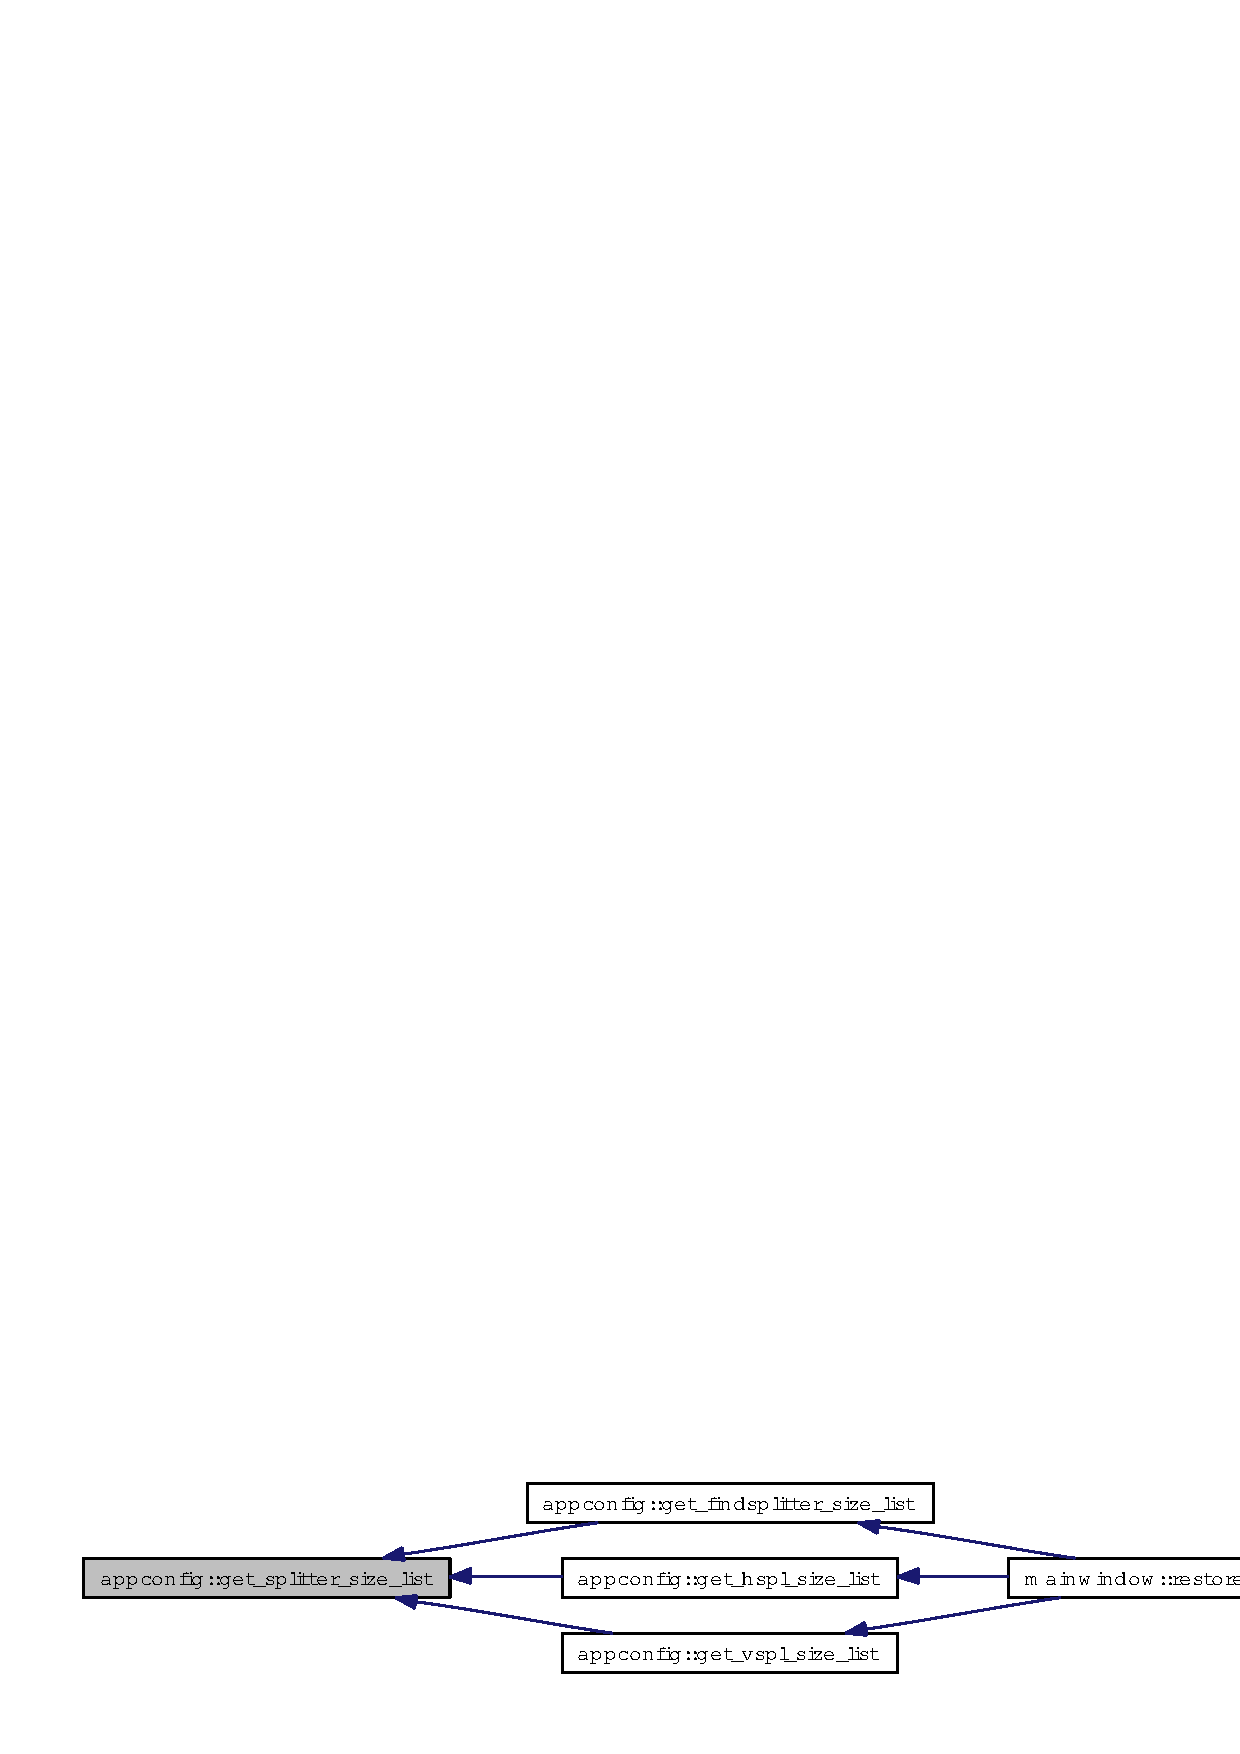
\includegraphics[width=371pt]{classappconfig_2e35d75471242db7840adf8058c861d4_icgraph}
\end{center}
\end{figure}
\index{appconfig@{appconfig}!set_splitter_size_list@{set\_\-splitter\_\-size\_\-list}}
\index{set_splitter_size_list@{set\_\-splitter\_\-size\_\-list}!appconfig@{appconfig}}
\subsubsection{\setlength{\rightskip}{0pt plus 5cm}void appconfig::set\_\-splitter\_\-size\_\-list (QString {\em name}, QList$<$ int $>$ {\em list})}\label{classappconfig_9034c4651468dc4fc51f85e790aae53e}




Definition at line 260 of file appconfig.cpp.

References conf.

Referenced by set\_\-findsplitter\_\-size\_\-list(), set\_\-hspl\_\-size\_\-list(), and set\_\-vspl\_\-size\_\-list().

Here is the caller graph for this function:\begin{figure}[H]
\begin{center}
\leavevmode
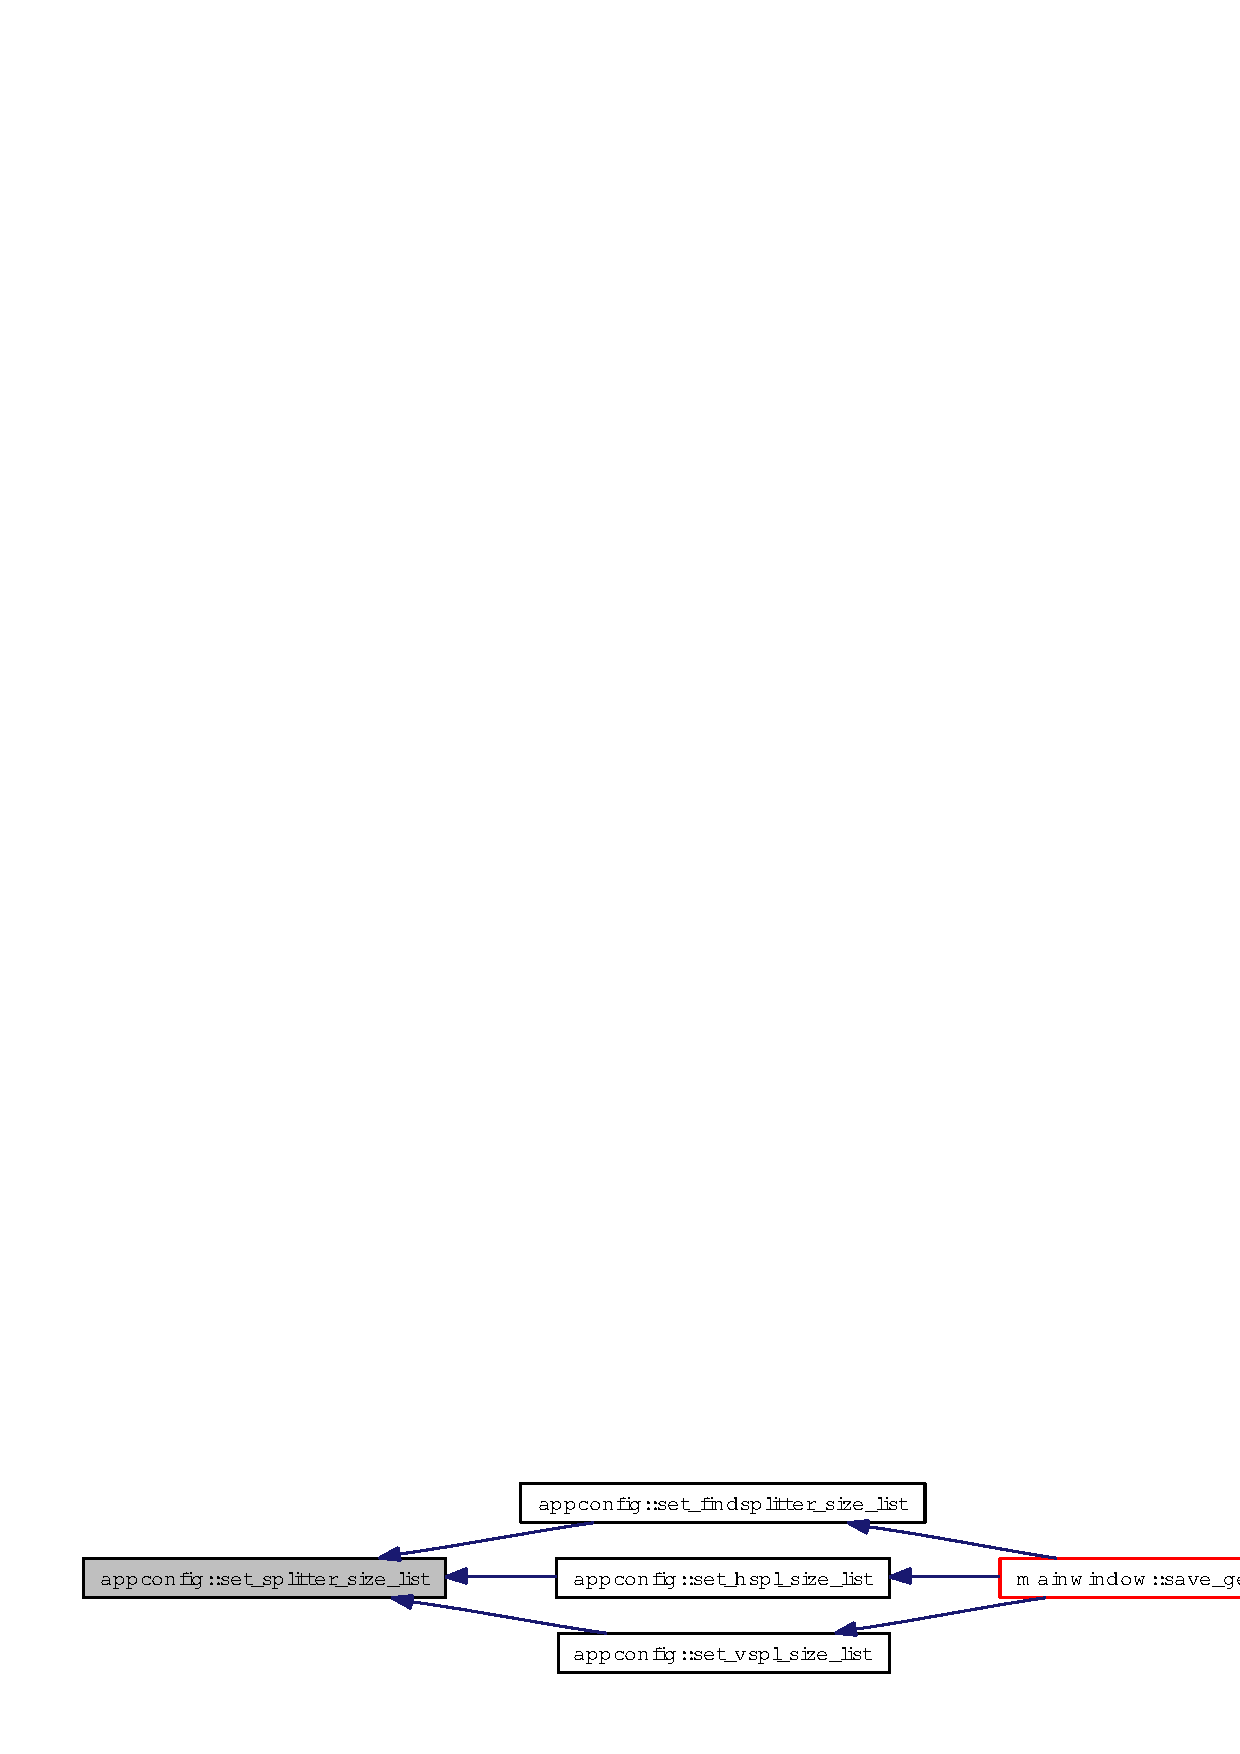
\includegraphics[width=324pt]{classappconfig_9034c4651468dc4fc51f85e790aae53e_icgraph}
\end{center}
\end{figure}
\index{appconfig@{appconfig}!get_tree_position@{get\_\-tree\_\-position}}
\index{get_tree_position@{get\_\-tree\_\-position}!appconfig@{appconfig}}
\subsubsection{\setlength{\rightskip}{0pt plus 5cm}QString\-List appconfig::get\_\-tree\_\-position (void)}\label{classappconfig_5b1150362b24baa90af6fed0df881289}




Definition at line 271 of file appconfig.cpp.

References conf.

Referenced by mainwindow::restore\_\-tree\_\-position().

Here is the caller graph for this function:\begin{figure}[H]
\begin{center}
\leavevmode
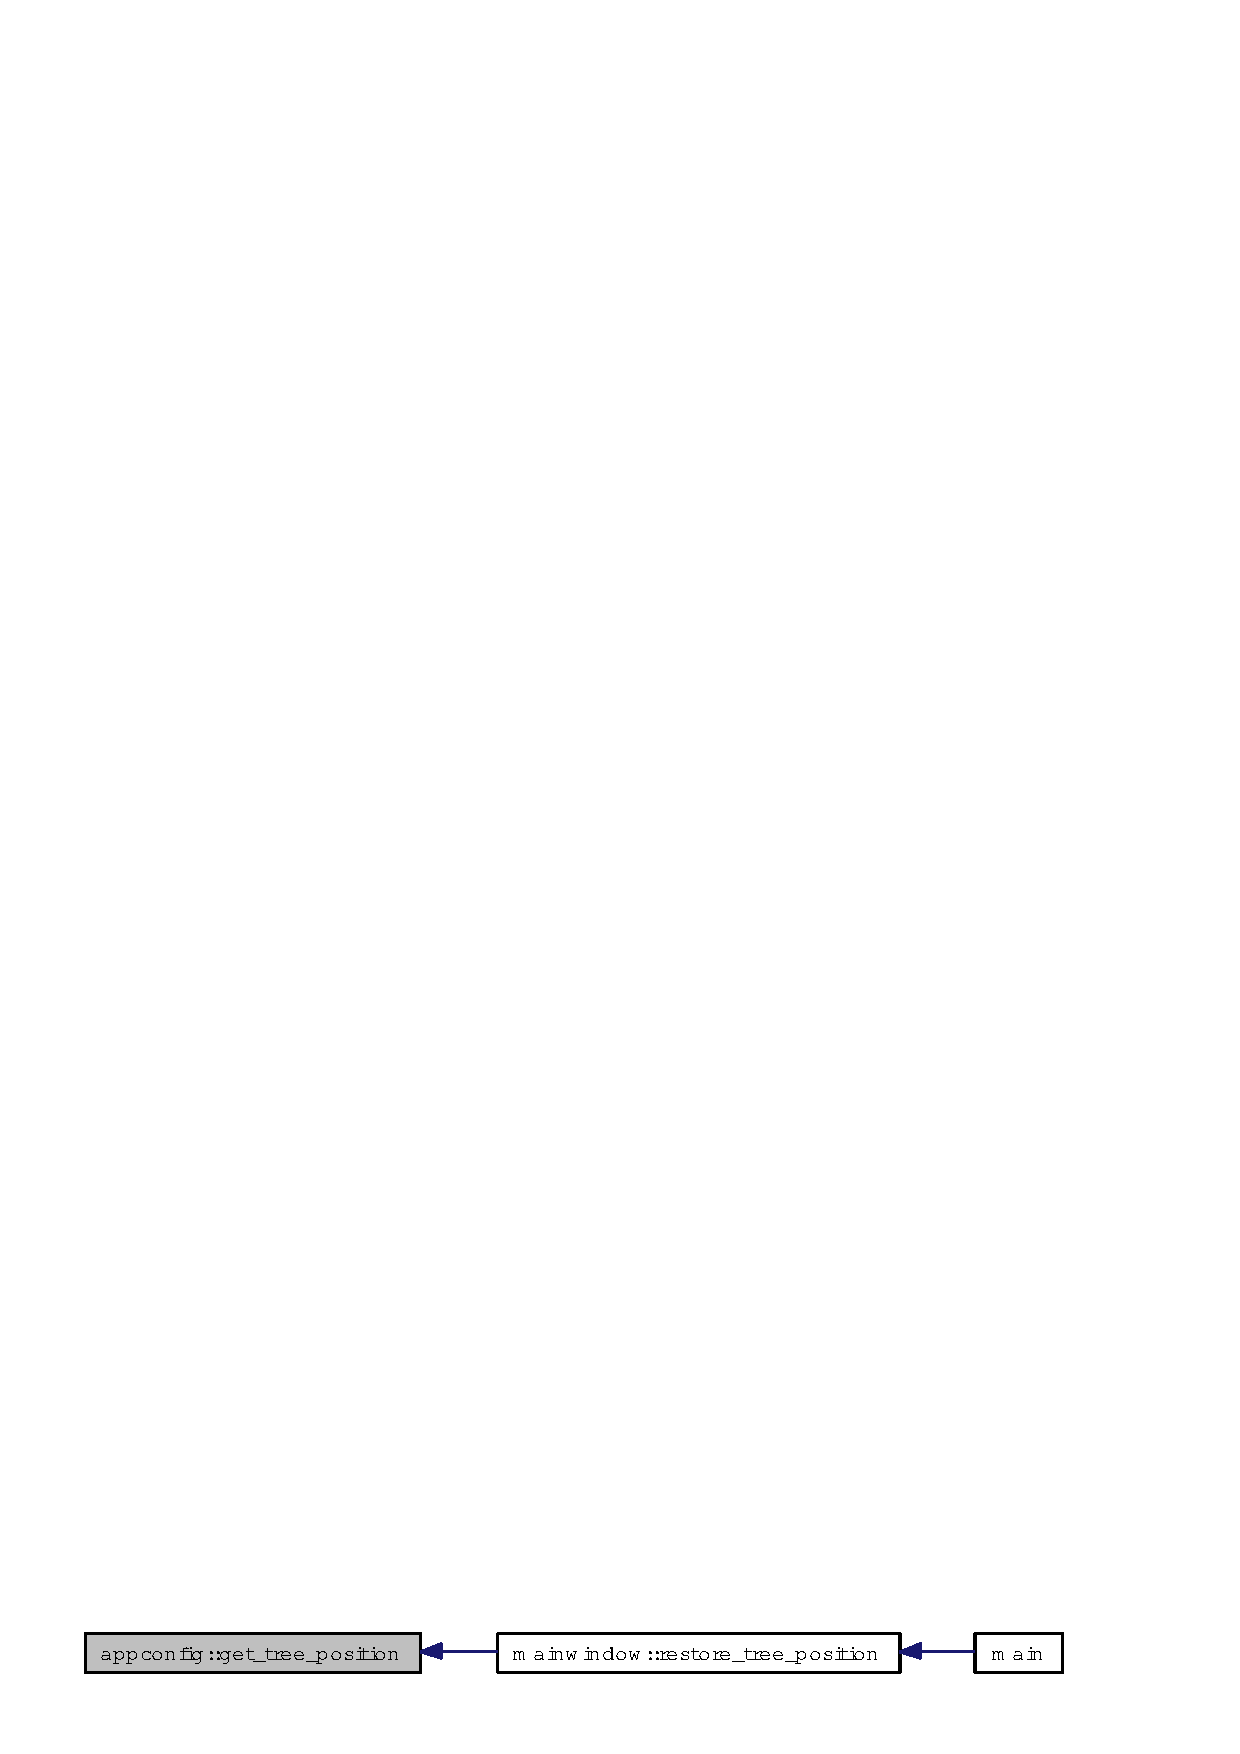
\includegraphics[width=257pt]{classappconfig_5b1150362b24baa90af6fed0df881289_icgraph}
\end{center}
\end{figure}
\index{appconfig@{appconfig}!set_tree_position@{set\_\-tree\_\-position}}
\index{set_tree_position@{set\_\-tree\_\-position}!appconfig@{appconfig}}
\subsubsection{\setlength{\rightskip}{0pt plus 5cm}void appconfig::set\_\-tree\_\-position (QString\-List {\em list})}\label{classappconfig_2861dee157700f295a4cf93236c8fba0}




Definition at line 277 of file appconfig.cpp.

References conf.

Referenced by mainwindow::save\_\-tree\_\-position().

Here is the caller graph for this function:\begin{figure}[H]
\begin{center}
\leavevmode
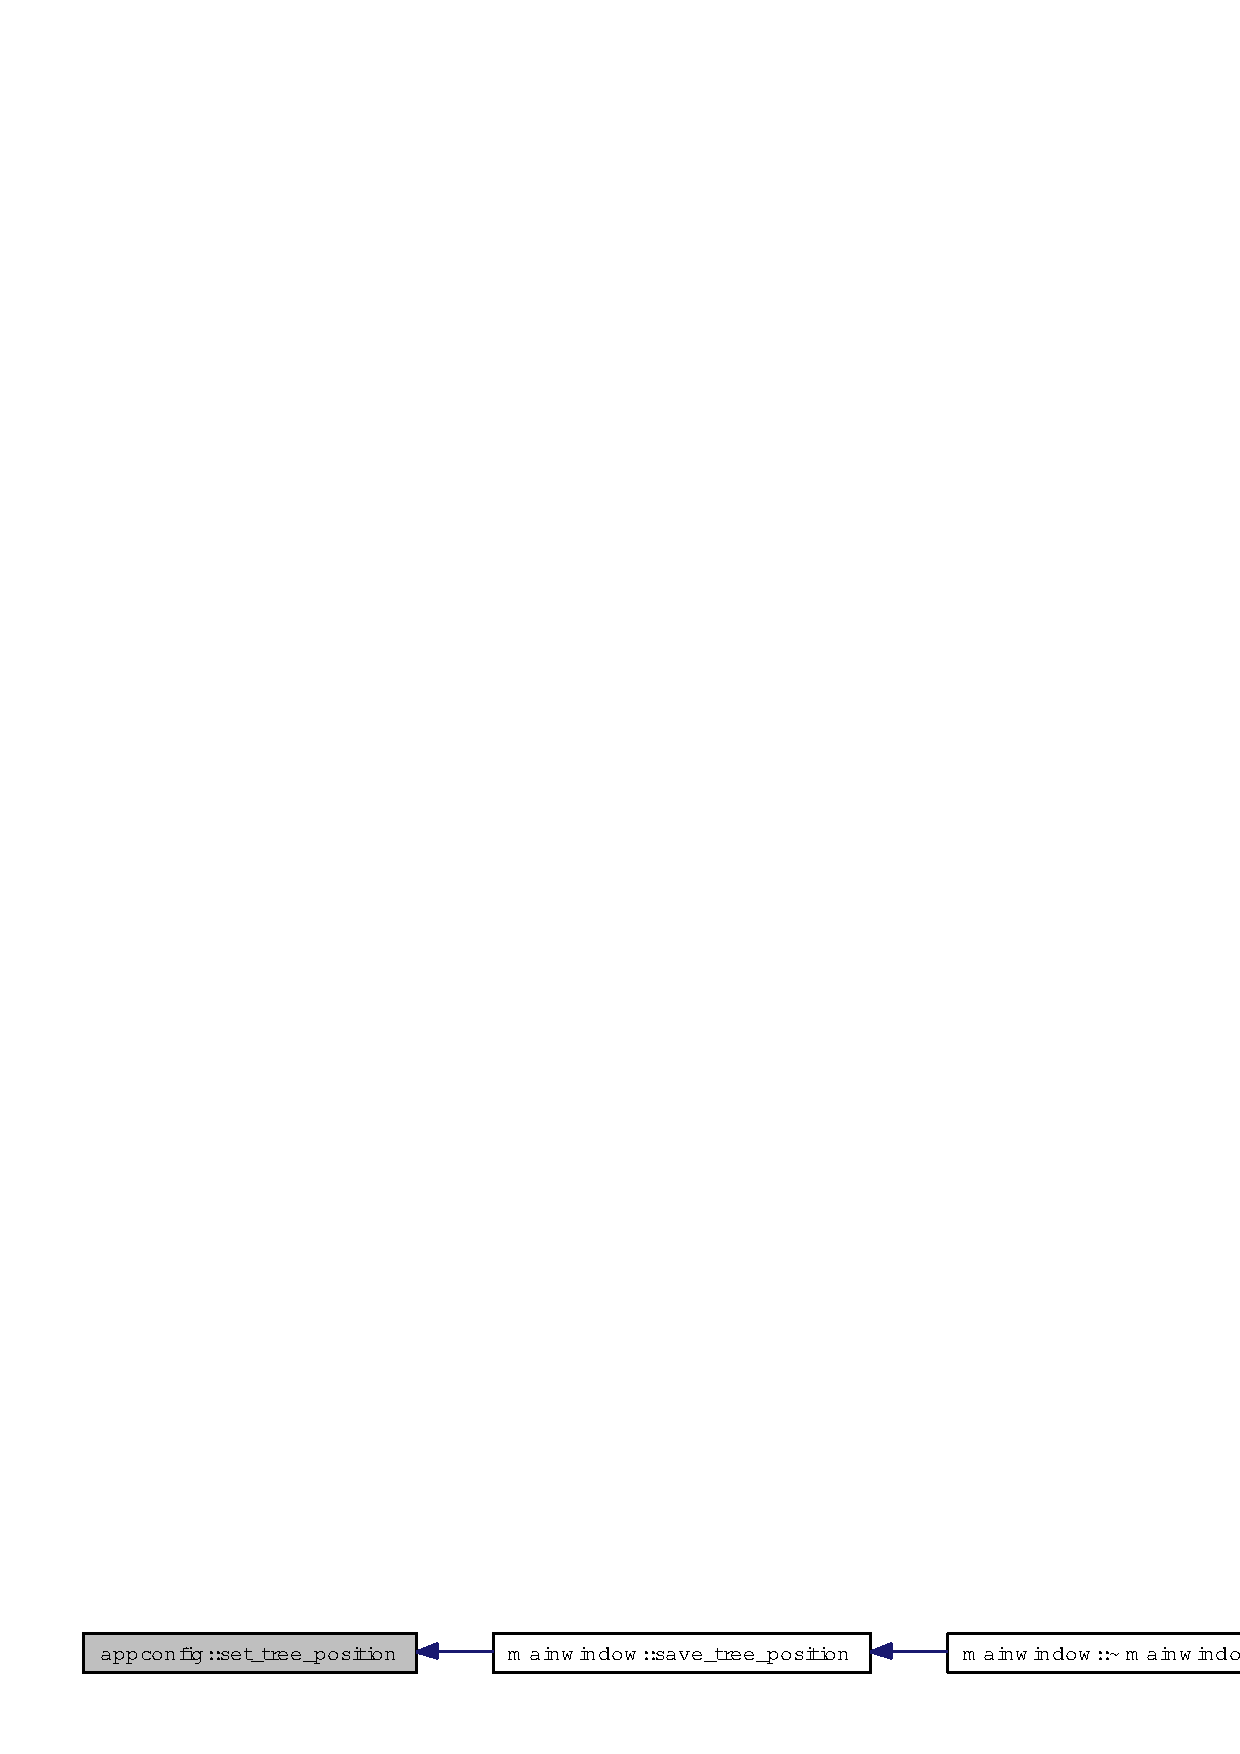
\includegraphics[width=309pt]{classappconfig_2861dee157700f295a4cf93236c8fba0_icgraph}
\end{center}
\end{figure}
\index{appconfig@{appconfig}!get_recordtable_position@{get\_\-recordtable\_\-position}}
\index{get_recordtable_position@{get\_\-recordtable\_\-position}!appconfig@{appconfig}}
\subsubsection{\setlength{\rightskip}{0pt plus 5cm}int appconfig::get\_\-recordtable\_\-position (void)}\label{classappconfig_28d3a670a10c4d0ef00f39a17db41bd3}




Definition at line 283 of file appconfig.cpp.

References conf.

Referenced by mainwindow::restore\_\-recordtable\_\-position().

Here is the caller graph for this function:\begin{figure}[H]
\begin{center}
\leavevmode
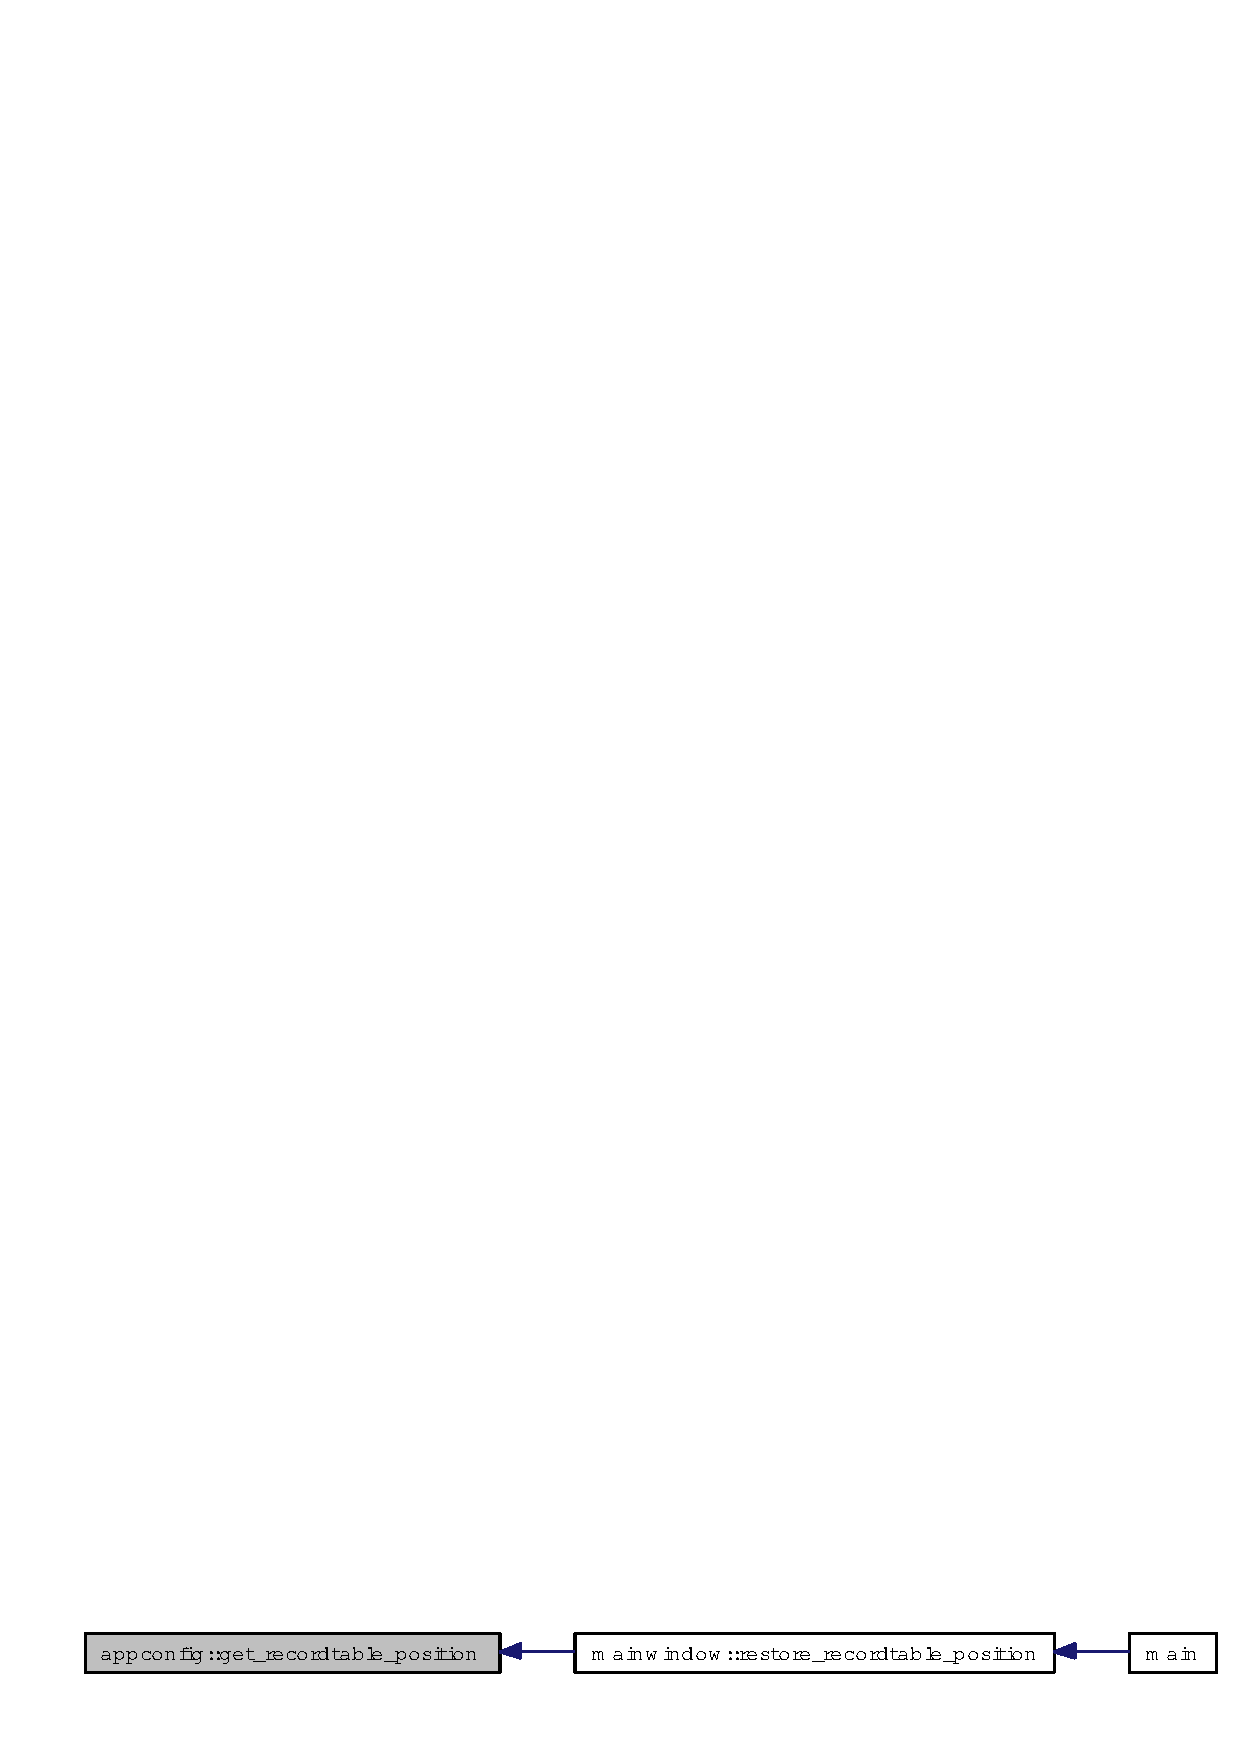
\includegraphics[width=294pt]{classappconfig_28d3a670a10c4d0ef00f39a17db41bd3_icgraph}
\end{center}
\end{figure}
\index{appconfig@{appconfig}!set_recordtable_position@{set\_\-recordtable\_\-position}}
\index{set_recordtable_position@{set\_\-recordtable\_\-position}!appconfig@{appconfig}}
\subsubsection{\setlength{\rightskip}{0pt plus 5cm}void appconfig::set\_\-recordtable\_\-position (int {\em pos})}\label{classappconfig_cad694c68b4fc41283b25be585633069}




Definition at line 289 of file appconfig.cpp.

References conf.

Referenced by mainwindow::save\_\-recordtable\_\-position().

Here is the caller graph for this function:\begin{figure}[H]
\begin{center}
\leavevmode
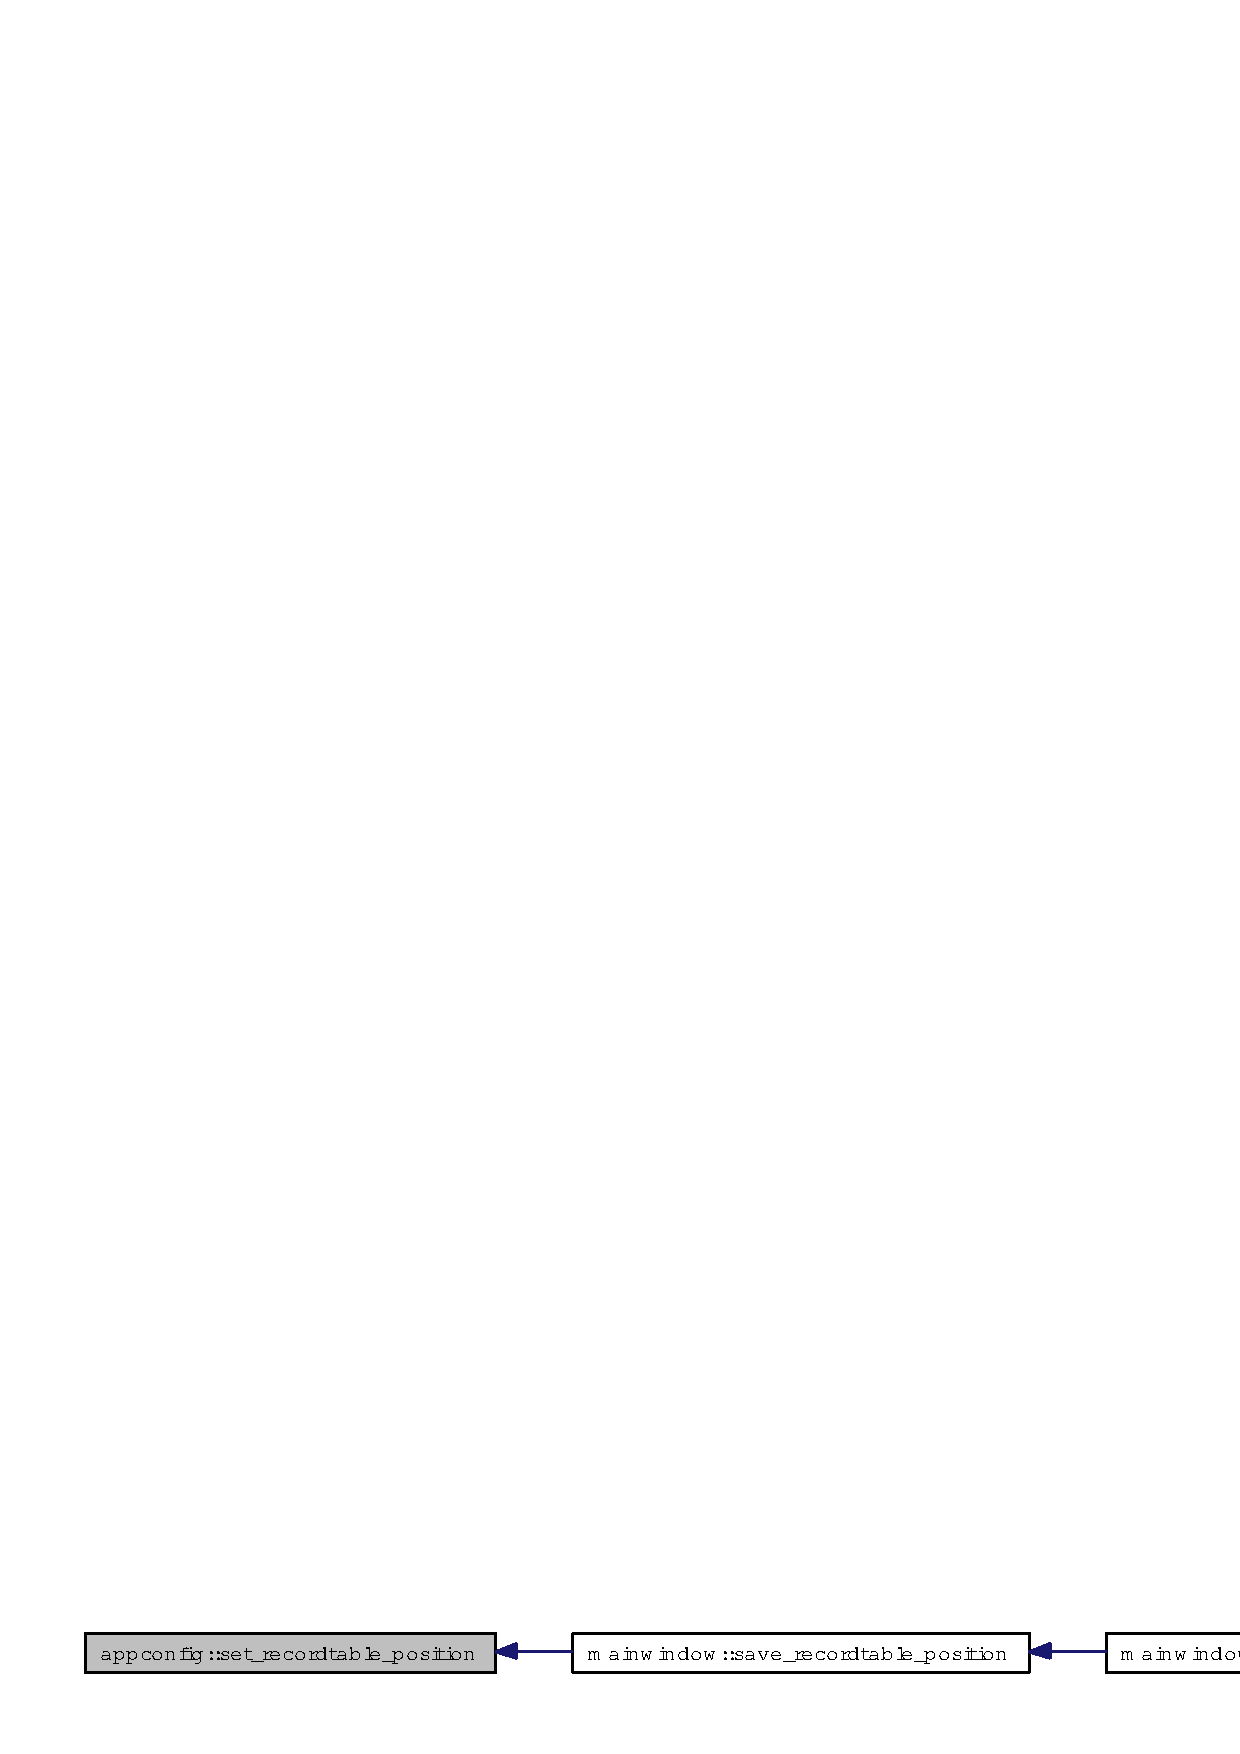
\includegraphics[width=347pt]{classappconfig_cad694c68b4fc41283b25be585633069_icgraph}
\end{center}
\end{figure}
\index{appconfig@{appconfig}!get_findscreen_wordregard@{get\_\-findscreen\_\-wordregard}}
\index{get_findscreen_wordregard@{get\_\-findscreen\_\-wordregard}!appconfig@{appconfig}}
\subsubsection{\setlength{\rightskip}{0pt plus 5cm}int appconfig::get\_\-findscreen\_\-wordregard (void)}\label{classappconfig_73adc21ab9840f316d9d3750709c193e}




Definition at line 295 of file appconfig.cpp.

References conf.

Referenced by findscreen::setup\_\-toolsline().

Here is the caller graph for this function:\begin{figure}[H]
\begin{center}
\leavevmode
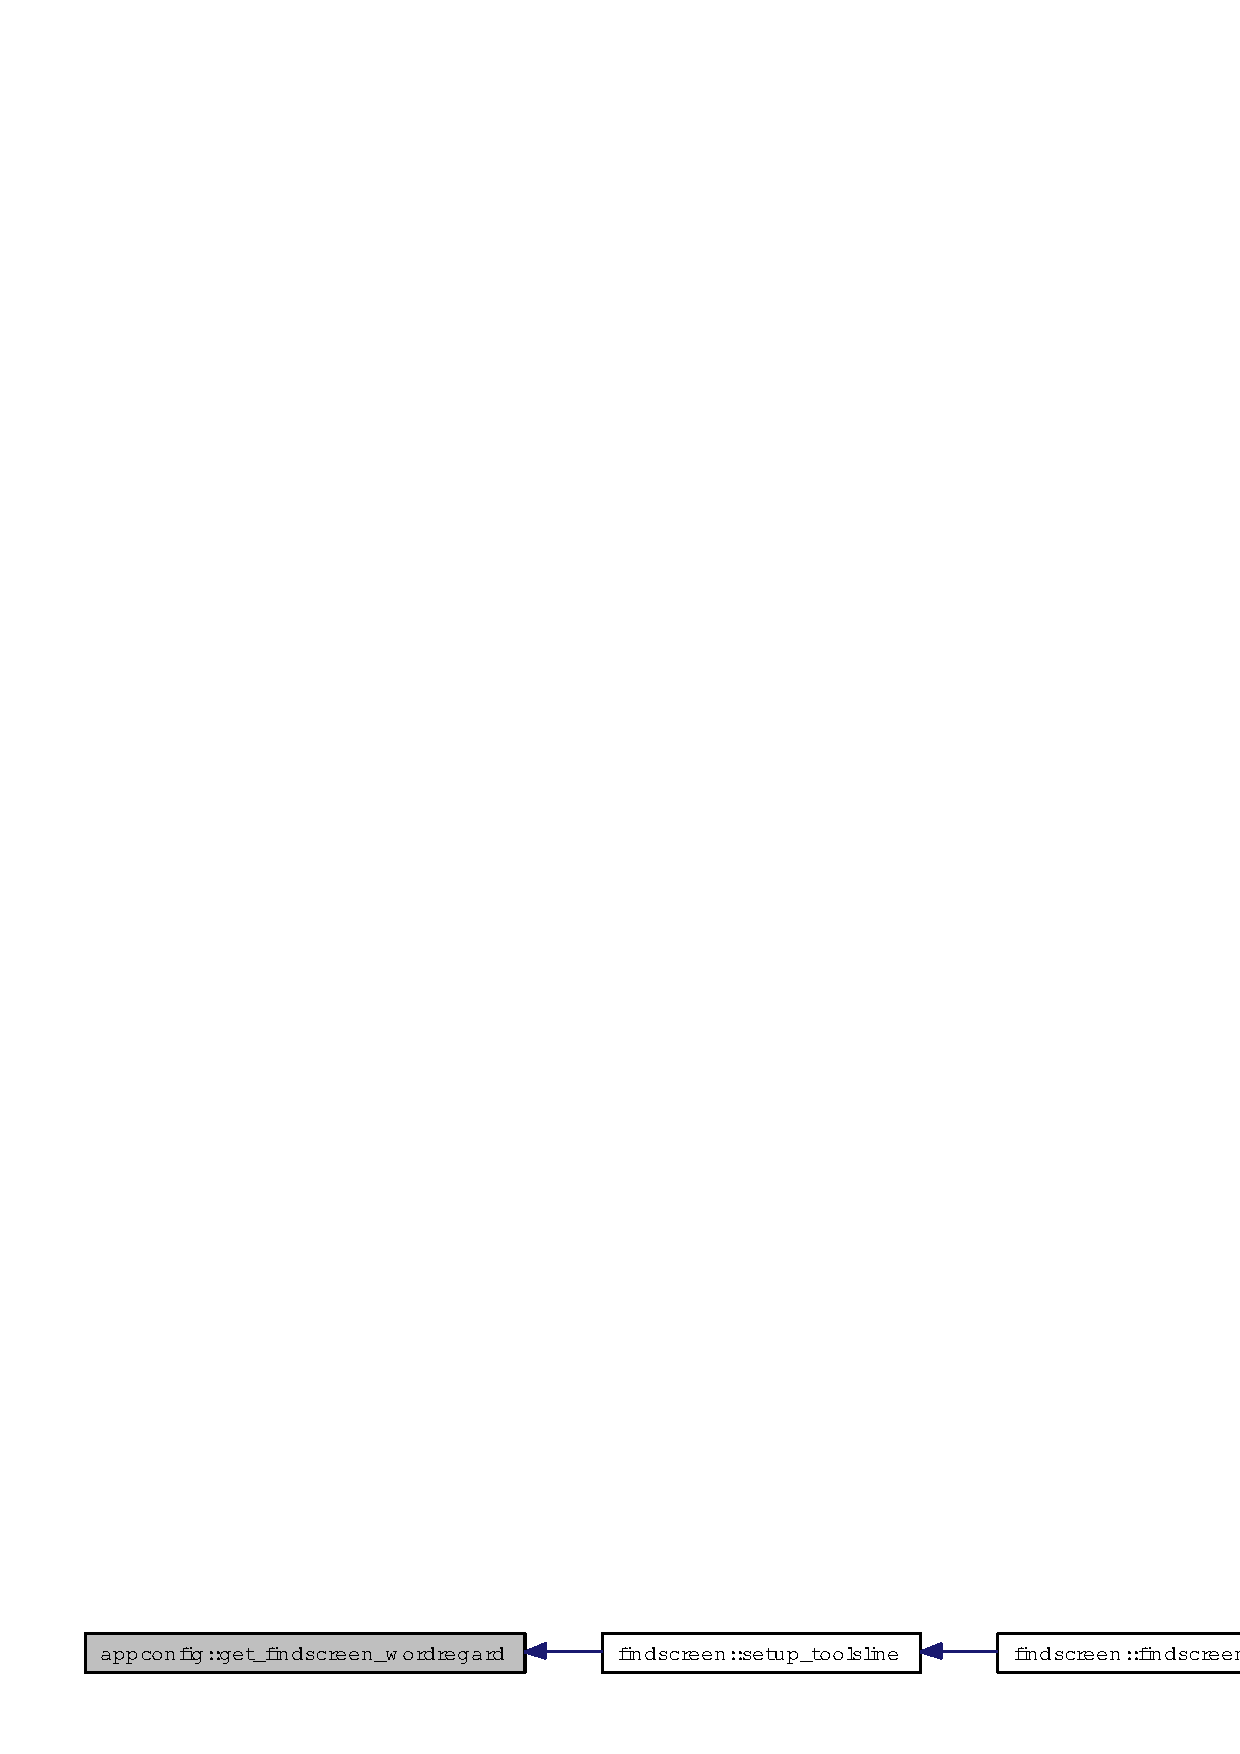
\includegraphics[width=306pt]{classappconfig_73adc21ab9840f316d9d3750709c193e_icgraph}
\end{center}
\end{figure}
\index{appconfig@{appconfig}!set_findscreen_wordregard@{set\_\-findscreen\_\-wordregard}}
\index{set_findscreen_wordregard@{set\_\-findscreen\_\-wordregard}!appconfig@{appconfig}}
\subsubsection{\setlength{\rightskip}{0pt plus 5cm}void appconfig::set\_\-findscreen\_\-wordregard (int {\em pos})}\label{classappconfig_09a324fbbbe567484dc5679f652c690d}




Definition at line 301 of file appconfig.cpp.

References conf.

Referenced by findscreen::changed\_\-wordregard().\index{appconfig@{appconfig}!get_findscreen_howextract@{get\_\-findscreen\_\-howextract}}
\index{get_findscreen_howextract@{get\_\-findscreen\_\-howextract}!appconfig@{appconfig}}
\subsubsection{\setlength{\rightskip}{0pt plus 5cm}int appconfig::get\_\-findscreen\_\-howextract (void)}\label{classappconfig_6b4dbe6b7dae577ac8264353675c8227}




Definition at line 307 of file appconfig.cpp.

References conf.

Referenced by findscreen::setup\_\-toolsline().

Here is the caller graph for this function:\begin{figure}[H]
\begin{center}
\leavevmode
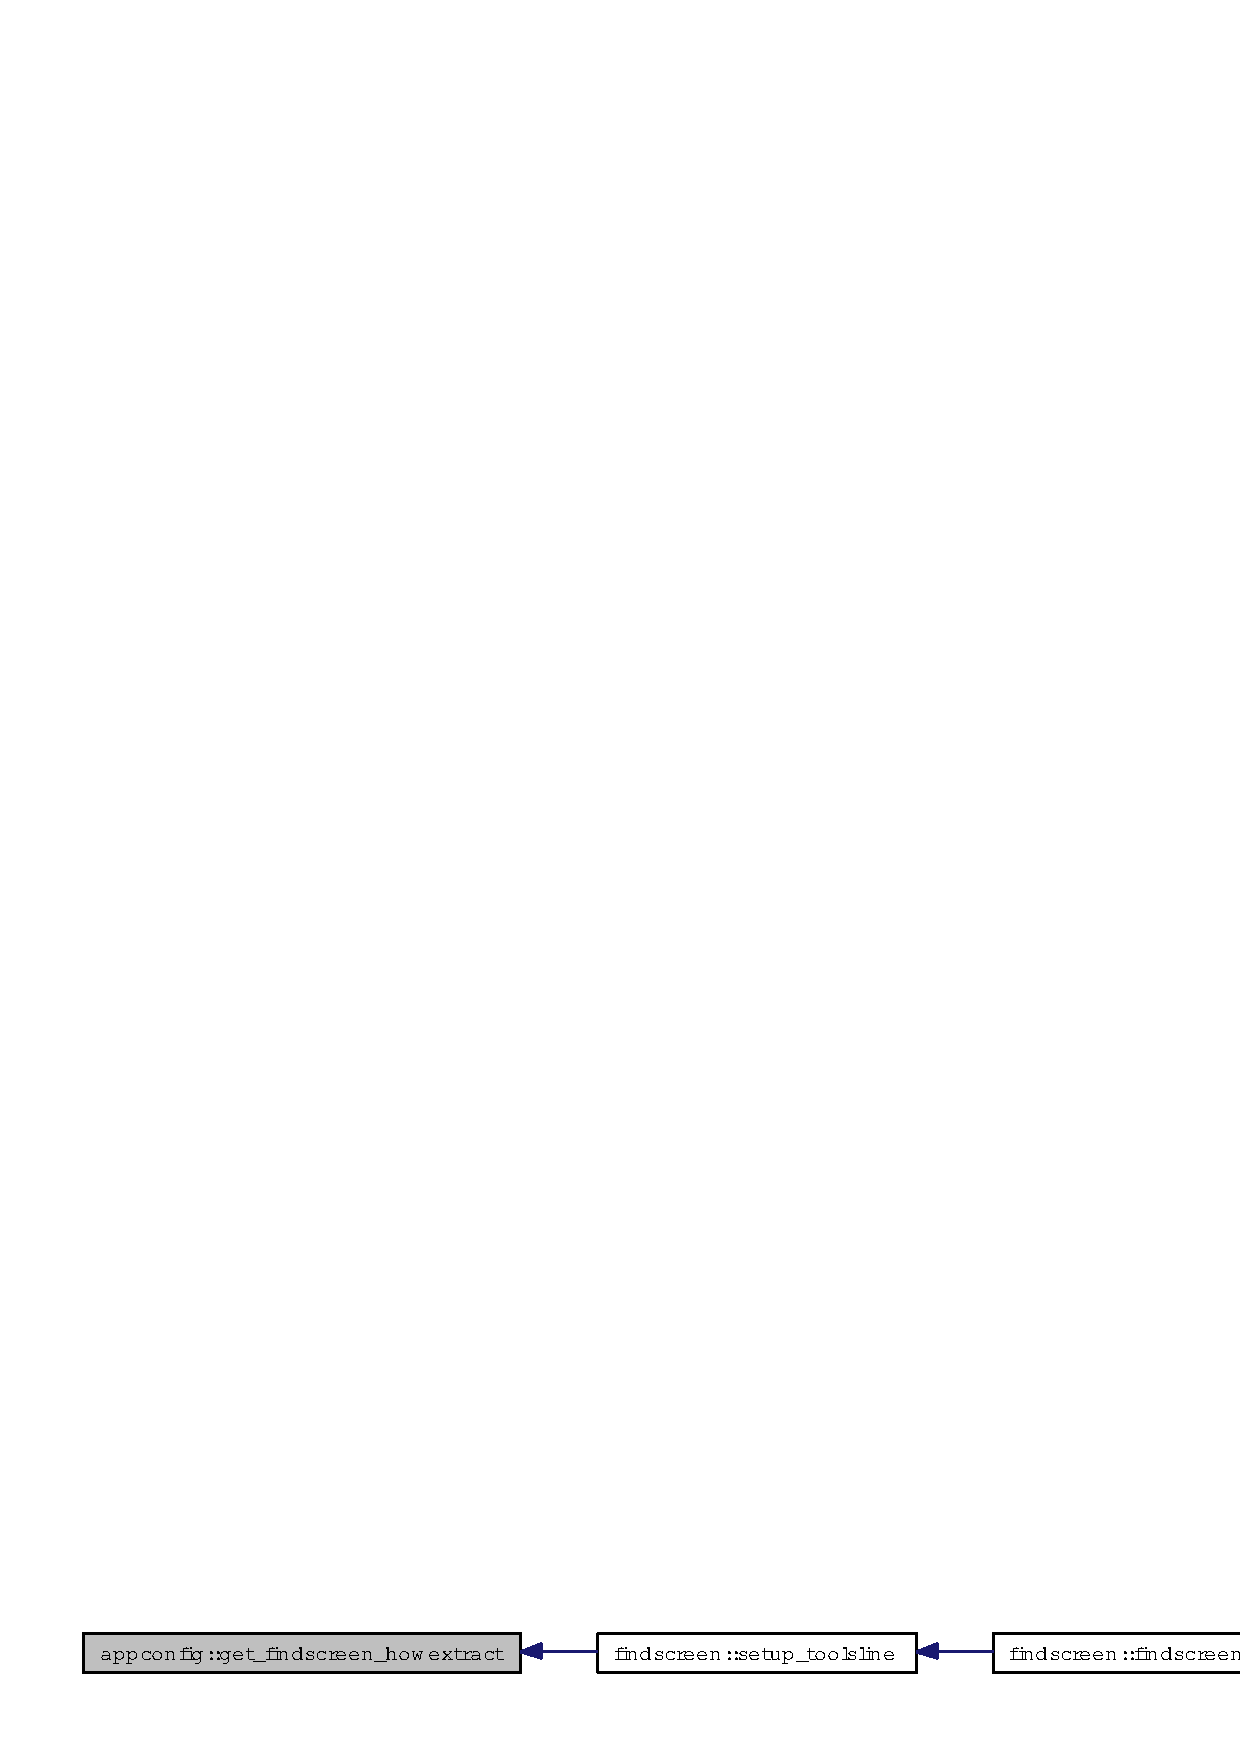
\includegraphics[width=305pt]{classappconfig_6b4dbe6b7dae577ac8264353675c8227_icgraph}
\end{center}
\end{figure}
\index{appconfig@{appconfig}!set_findscreen_howextract@{set\_\-findscreen\_\-howextract}}
\index{set_findscreen_howextract@{set\_\-findscreen\_\-howextract}!appconfig@{appconfig}}
\subsubsection{\setlength{\rightskip}{0pt plus 5cm}void appconfig::set\_\-findscreen\_\-howextract (int {\em pos})}\label{classappconfig_5e7575dcf4b71cf2860782b907a0eadc}




Definition at line 313 of file appconfig.cpp.

References conf.

Referenced by findscreen::changed\_\-howextract().\index{appconfig@{appconfig}!get_findscreen_find_in_field@{get\_\-findscreen\_\-find\_\-in\_\-field}}
\index{get_findscreen_find_in_field@{get\_\-findscreen\_\-find\_\-in\_\-field}!appconfig@{appconfig}}
\subsubsection{\setlength{\rightskip}{0pt plus 5cm}bool appconfig::get\_\-findscreen\_\-find\_\-in\_\-field (QString {\em fieldname})}\label{classappconfig_87e86c00befff9437750da73f9ef0880}




Definition at line 319 of file appconfig.cpp.

References conf.

Referenced by findscreen::setup\_\-wherefindline().

Here is the caller graph for this function:\begin{figure}[H]
\begin{center}
\leavevmode
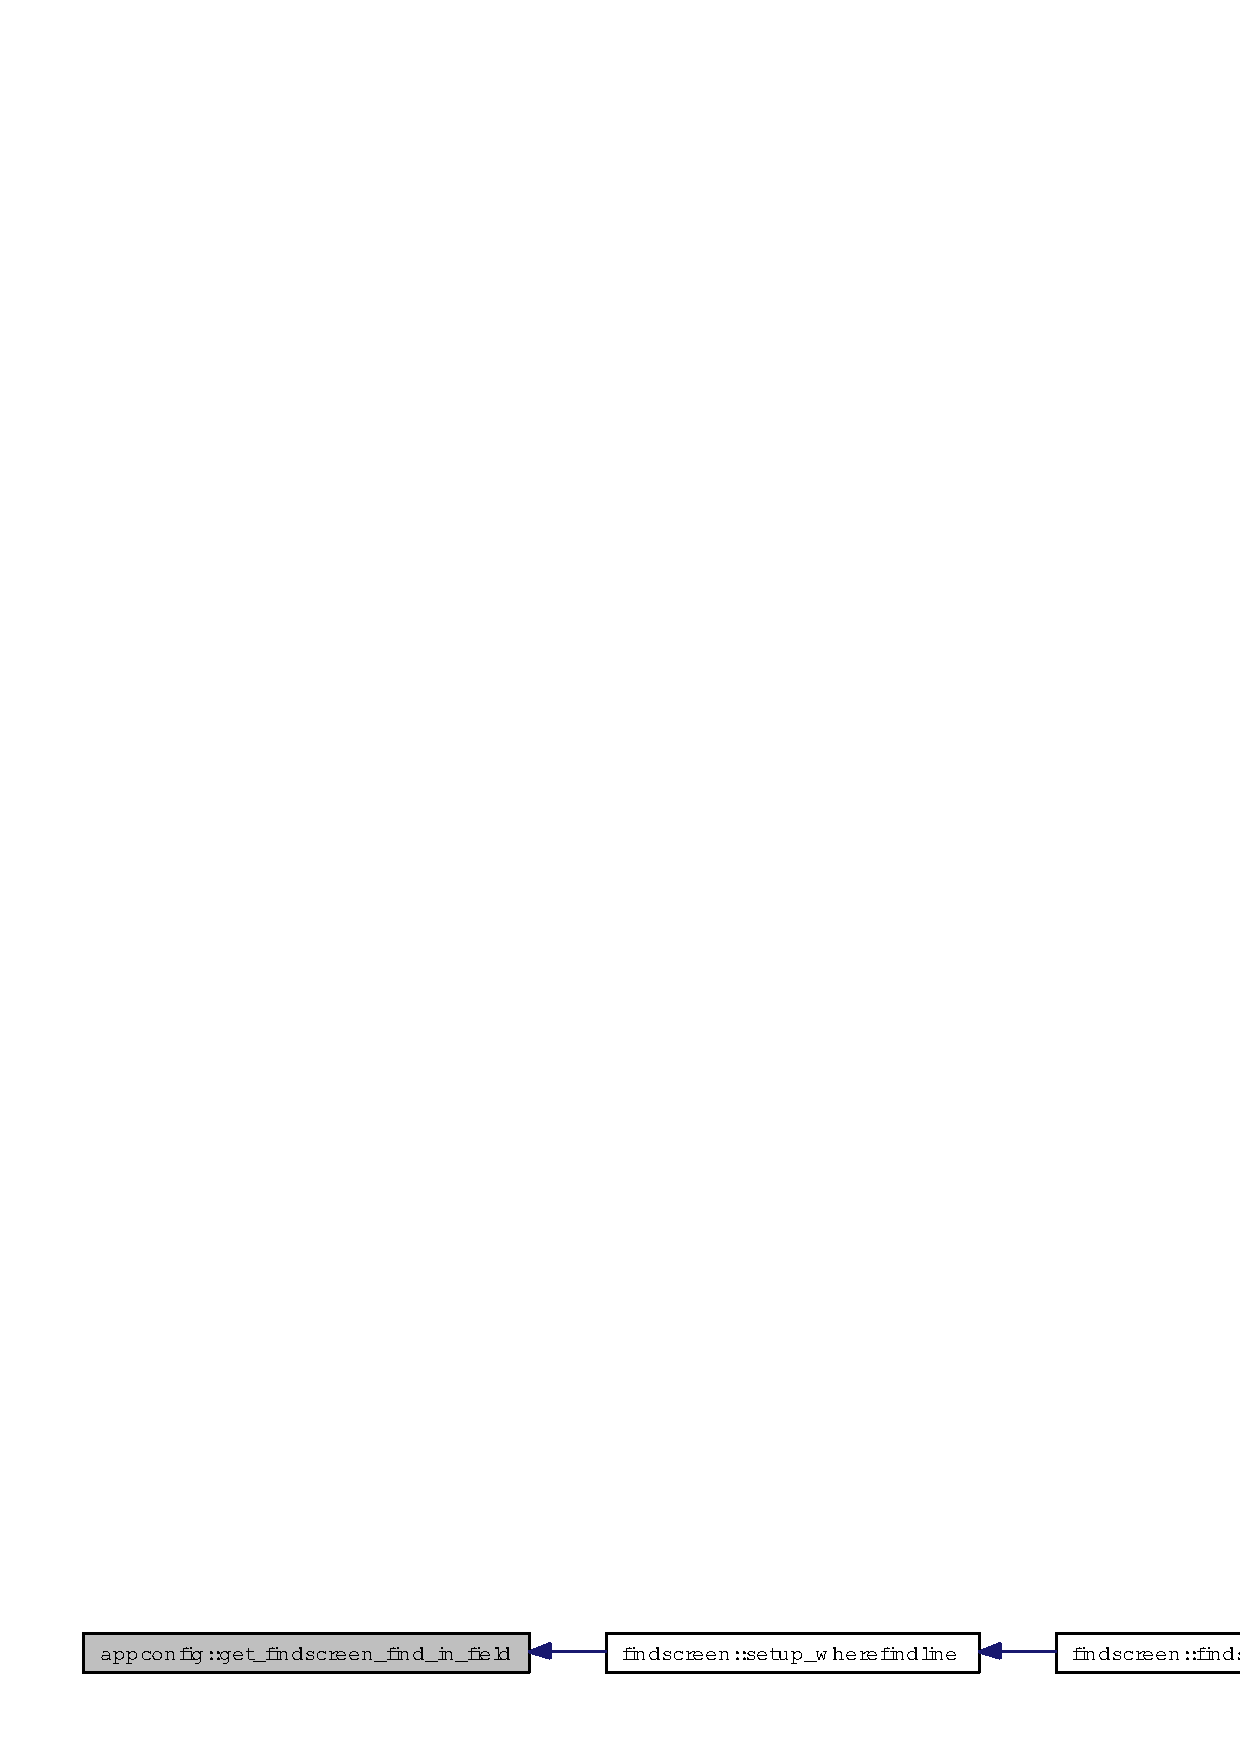
\includegraphics[width=320pt]{classappconfig_87e86c00befff9437750da73f9ef0880_icgraph}
\end{center}
\end{figure}
\index{appconfig@{appconfig}!set_findscreen_find_in_field@{set\_\-findscreen\_\-find\_\-in\_\-field}}
\index{set_findscreen_find_in_field@{set\_\-findscreen\_\-find\_\-in\_\-field}!appconfig@{appconfig}}
\subsubsection{\setlength{\rightskip}{0pt plus 5cm}void appconfig::set\_\-findscreen\_\-find\_\-in\_\-field (QString {\em fieldname}, bool {\em ischecked})}\label{classappconfig_5f7bdbefcb85033c9e0a92a02df38010}




Definition at line 325 of file appconfig.cpp.

References conf.

Referenced by findscreen::changed\_\-find\_\-in\_\-field().

Here is the caller graph for this function:\begin{figure}[H]
\begin{center}
\leavevmode
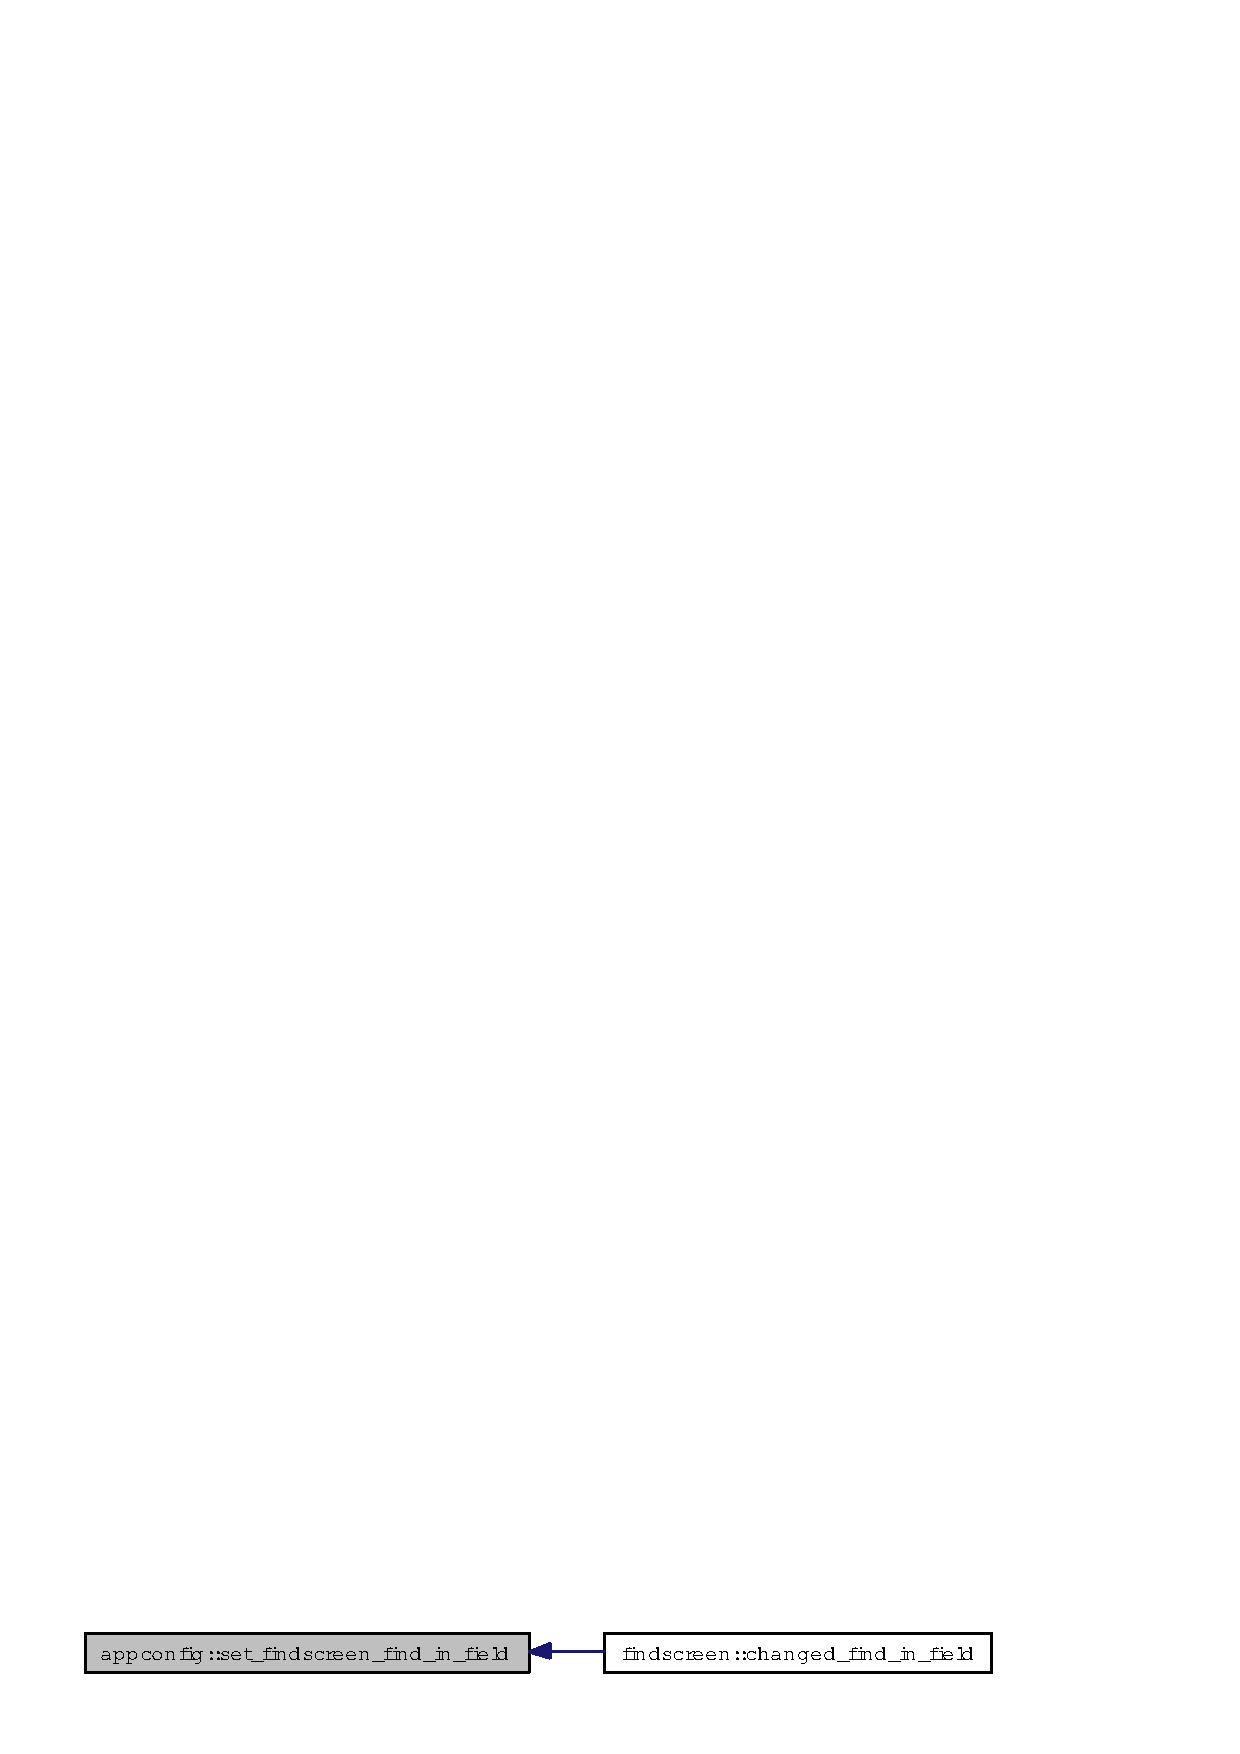
\includegraphics[width=240pt]{classappconfig_5f7bdbefcb85033c9e0a92a02df38010_icgraph}
\end{center}
\end{figure}
\index{appconfig@{appconfig}!get_findscreen_show@{get\_\-findscreen\_\-show}}
\index{get_findscreen_show@{get\_\-findscreen\_\-show}!appconfig@{appconfig}}
\subsubsection{\setlength{\rightskip}{0pt plus 5cm}bool appconfig::get\_\-findscreen\_\-show (void)}\label{classappconfig_056484ddd724fd4f30887a5087658d52}




Definition at line 331 of file appconfig.cpp.

References conf.

Referenced by mainwindow::restore\_\-findonbase\_\-visible().

Here is the caller graph for this function:\begin{figure}[H]
\begin{center}
\leavevmode
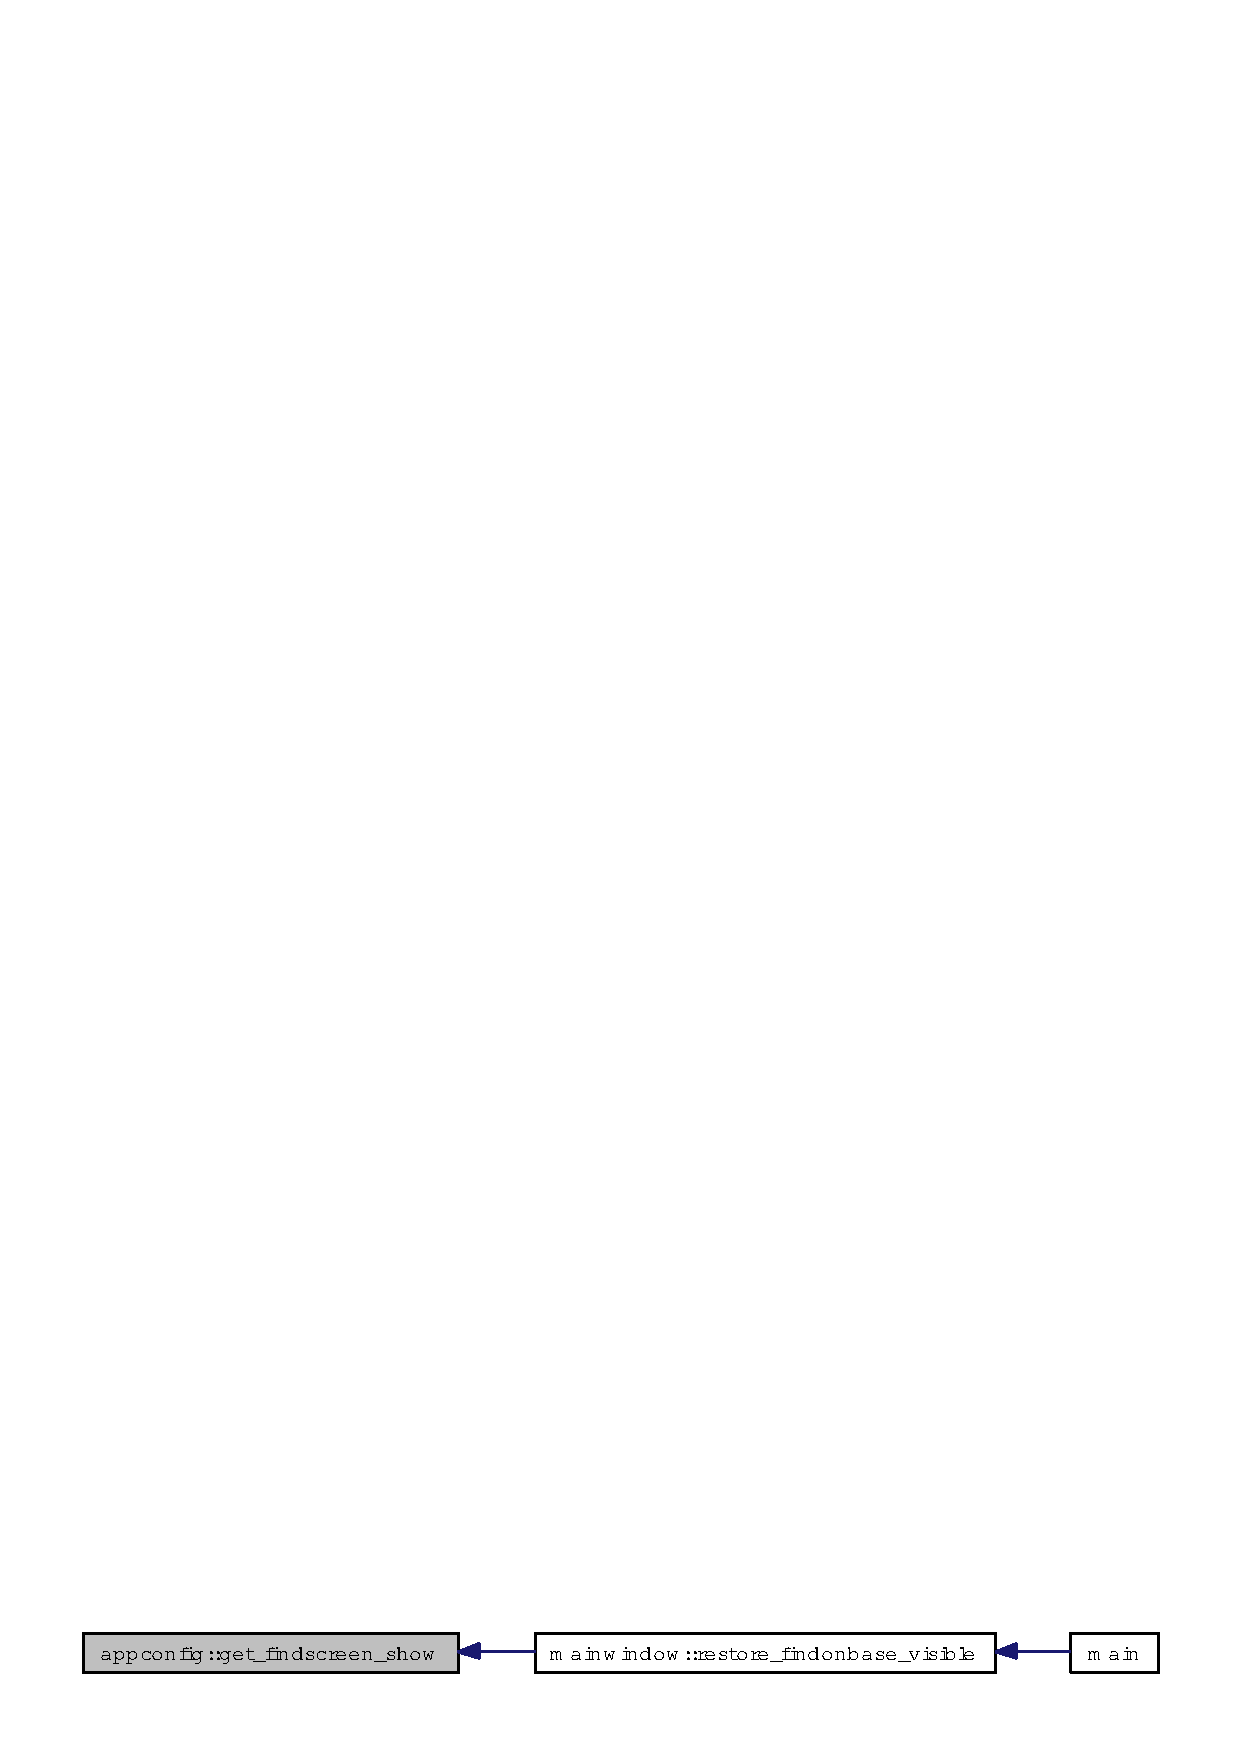
\includegraphics[width=280pt]{classappconfig_056484ddd724fd4f30887a5087658d52_icgraph}
\end{center}
\end{figure}
\index{appconfig@{appconfig}!set_findscreen_show@{set\_\-findscreen\_\-show}}
\index{set_findscreen_show@{set\_\-findscreen\_\-show}!appconfig@{appconfig}}
\subsubsection{\setlength{\rightskip}{0pt plus 5cm}void appconfig::set\_\-findscreen\_\-show (bool {\em isshow})}\label{classappconfig_45b5ebfaea239d18dcaab5ba29293e6a}




Definition at line 337 of file appconfig.cpp.

References conf.

Referenced by findscreen::widget\_\-hide(), and findscreen::widget\_\-show().\index{appconfig@{appconfig}!get_parameter@{get\_\-parameter}}
\index{get_parameter@{get\_\-parameter}!appconfig@{appconfig}}
\subsubsection{\setlength{\rightskip}{0pt plus 5cm}QString appconfig::get\_\-parameter (QString)\hspace{0.3cm}{\tt  [private]}}\label{classappconfig_d2db70d1978d1ca2bc0091a712ba641f}




Definition at line 34 of file appconfig.cpp.

References conf, and critical\_\-error().

Referenced by get\_\-addnewrecord\_\-expand\_\-info(), get\_\-lastidnum(), get\_\-lastnotenum(), get\_\-lastnotenum\_\-as\_\-line(), get\_\-lastprefixnum(), get\_\-lastprefixnum\_\-as\_\-line(), get\_\-tetradir(), and get\_\-trashdir().

Here is the call graph for this function:\begin{figure}[H]
\begin{center}
\leavevmode
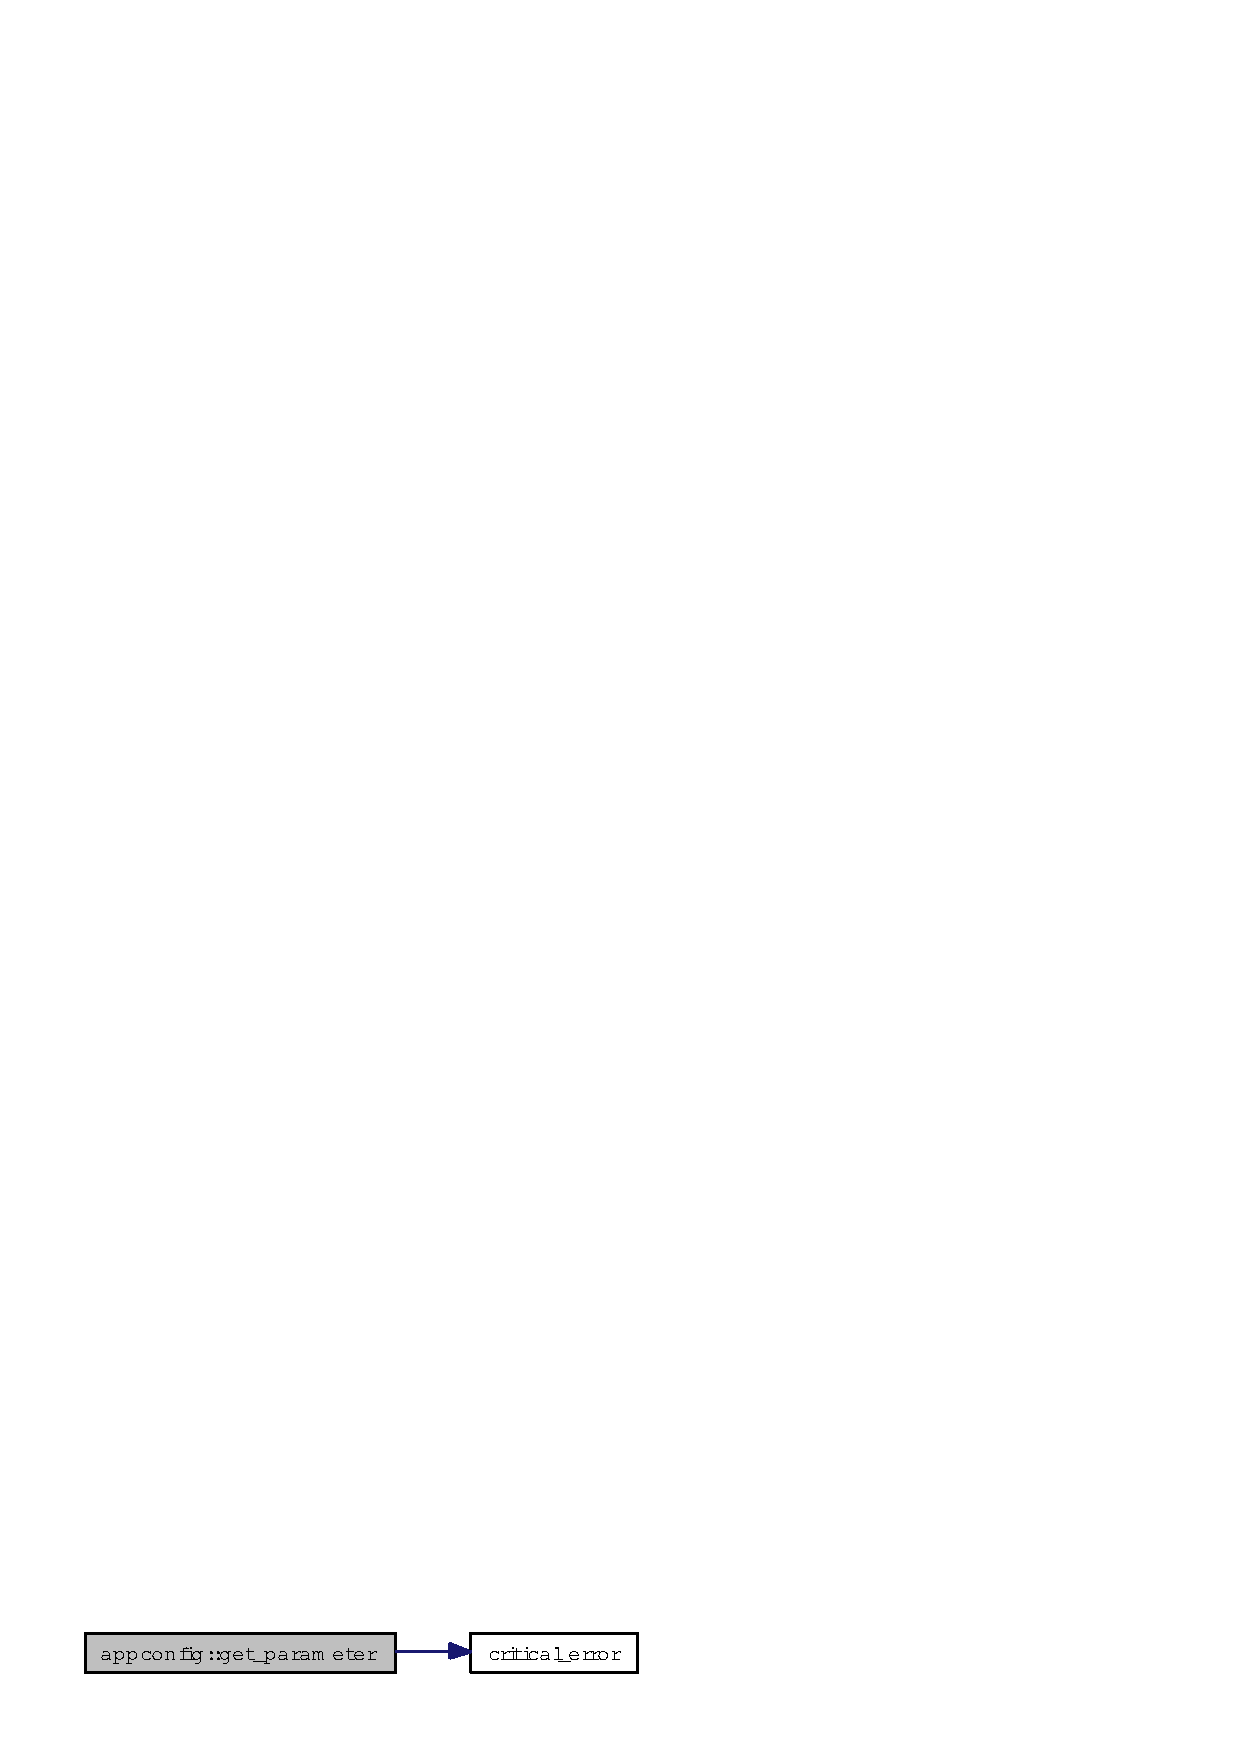
\includegraphics[width=155pt]{classappconfig_d2db70d1978d1ca2bc0091a712ba641f_cgraph}
\end{center}
\end{figure}


Here is the caller graph for this function:\begin{figure}[H]
\begin{center}
\leavevmode
\includegraphics[width=233pt]{classappconfig_d2db70d1978d1ca2bc0091a712ba641f_icgraph}
\end{center}
\end{figure}


\subsection{Member Data Documentation}
\index{appconfig@{appconfig}!conf@{conf}}
\index{conf@{conf}!appconfig@{appconfig}}
\subsubsection{\setlength{\rightskip}{0pt plus 5cm}QSettings {\bf appconfig::conf}\hspace{0.3cm}{\tt  [static, private]}}\label{classappconfig_753e9d9be9b93c732723b861a9a354b8}




Definition at line 84 of file appconfig.h.

Referenced by appconfig(), get\_\-findscreen\_\-find\_\-in\_\-field(), get\_\-findscreen\_\-howextract(), get\_\-findscreen\_\-show(), get\_\-findscreen\_\-wordregard(), get\_\-mainwingeometry(), get\_\-parameter(), get\_\-recordtable\_\-position(), get\_\-splitter\_\-size\_\-list(), get\_\-tree\_\-position(), inc\_\-lastidnum(), inc\_\-lastnotenum(), inc\_\-lastprefixnum(), set\_\-addnewrecord\_\-expand\_\-info(), set\_\-findscreen\_\-find\_\-in\_\-field(), set\_\-findscreen\_\-howextract(), set\_\-findscreen\_\-show(), set\_\-findscreen\_\-wordregard(), set\_\-mainwingeometry(), set\_\-recordtable\_\-position(), set\_\-splitter\_\-size\_\-list(), set\_\-tetradir(), set\_\-trashdir(), and set\_\-tree\_\-position().

The documentation for this class was generated from the following files:\begin{CompactItemize}
\item 
{\bf appconfig.h}\item 
{\bf appconfig.cpp}\end{CompactItemize}
